\documentclass[../thesis.tex]{subfiles}

\begin{document}

\chapter{Background subtraction}
\label{chap:bkg}

While Daya Bay's design ensures a very pure sample of antineutrino events, a small contamination of backgrounds (at the percent level) is unavoidable. These backgrounds can be subdivided into \emph{correlated} and \emph{uncorrelated} backgrounds. The uncorrelated backgrounds consist entirely of accidental coincidences between singles events, and the rate and spectrum can be easily estimated from that of the singles (see \autoref{sec:accratecalc}). On the other hand, the correlated backgrounds are so named because the prompt and delayed pulses are correlated in time and space, as they both originate from a single underlying process. The correlated background in Daya Bay consists of four distinct processes, and each one requires its own technique for determining the rate and energy spectrum.

In this chapter, we discuss the measurement of each of these backgrounds. Once they have been measured, their scaled prompt spectra can be subtracted from that of the IBD candidates, allowing the oscillation fit to proceed with a purer prompt spectrum, albeit one with an additional uncertainty stemming from the background measurements. We carry out our own prediction of the rates of accidental and $^9$Li/$^8$He backgrounds. For the three other backgrounds, we use the results of the detailed studies that were carried out by members of the collaboration.

Before considering these double-coincidence backgrounds, we begin by discussing a background defined at the level of \emph{individual} triggers, namely, the so-called ``flashing'' of PMTs. Reduction of these ``flashers'' is necessary in order to minimize the rate of the uncorrelated backgrounds. This reduction occurs at an early stage in the analysis (the ``pre-selection'', as described in \autoref{sec:selPreSel}), eliminating flashers entirely from further consideration.

\section{PMT light emission (``flashers'')}
\label{sec:bkgFlashers}

During detector commissioning, most PMTs were found to occasionally emit varying amount of light due to arcing in their bases. The rate and intensity of this ``flashing'' would change over time for each PMT. At any given moment, some 5\% of the PMTs in each AD will have the tendency to flash brightly enough to trigger the detector \cite{SideBySide}, in some cases producing as much as 100~MeV of reconstructed energy. Within the delayed energy region of 6-12~MeV, the flasher rate has averaged at around 0.7~Hz for each AD. These ``delayed-like'' flashers, if included in the analysis, would significantly increase the rate of backgrounds caused by the accidental coincidence of two uncorrelated signals. As discussed in \autoref{sec:accbkg} and \autoref{chap:accDMC}, the rate of such ``accidentals'' is proportional to the rate of delayed-like signals, and this rate (excluding flashers) ranges from around 0.05~Hz at EH3 to 1~Hz at EH1. While the flashers would merely (roughly) double the 1\% accidental background in the near halls, in the far hall it would increase this background by an order of magnitude to the 10\% level, counter to Daya Bay's goal of perecent-level background contamination.

Fortunately, flashers are easily distinguished from ``physical'' singles due to their unique pattern of light emission, enabling them to be removed from the analysis with high efficiency while minimally affecting true IBDs. This light pattern is characteristized by two ``hot spots'' on opposite sides of the AD. When a PMT base emits light, much of the light is absorbed by the black radial shield and the conical magnetic shield. The remainder escapes within a conical profile; some of the photons will strike the flasher's photocathode (resulting in the flashing PMT having the highest charge), and others will primarily illuminate the PMTs across the AD from the flasher, especially the one that lies directly opposite to it. In addition, the time distribution of the PMT hits is broadened for flashers due to the geometry of light propagation across the AD. By taking advantage of these telltale distributions of charges and times, it is possible to achieve excellent discrimination of flashers from physical events.

The flasher identification criteria were developed in a somewhat ad-hoc fashion, by defining quantities that could conceivably serve as discriminators, and then further defining combinations of these quantities, and finally plotting the distributions of these (combined) quantities until a clean separation between flashers and non-flashers was apparent. It is far more important to minimize (IBD) signal inefficiency instead of maximizing flasher rejection, because a small amount of unrejected flashers will simply slightly increase the rate of accidental backgrounds (which can be easily quantified), whereas a signal inefficiency could vary among the ADs and thereby bias the oscillation fit.

\newcommand\fmax{f_{\mathrm{max}}}
\newcommand\fquad{f_{\mathrm{quad}}}
\newcommand\fID{f_{\mathrm{ID}}}
\newcommand\fPSD{f_{\mathrm{PSD}}}

Early in the experiment, this prolonged and interative process eventually gave rise to the \emph{ellipse cut} (based on the charge distribution) and the \emph{PSD cut} (based on the time distribution), which demonstrated excellent performance, and these cuts continue to be used in this analysis. The ellipse cut is based on two quantities, termed $\fmax$ and $\fquad$. The first, $\fmax$, is simply the ratio of $Q_{\mathrm{max}}$ (the maximum individual PMT charge across all PMTs) over the total charge $Q_{\mathrm{tot}}$:
\begin{equation}
  \fmax = \frac{Q_{\mathrm{max}}}{Q_{\mathrm{tot}}}.
\end{equation}
For flasher events, $Q_{\mathrm{max}}$ belongs to the flashing PMT itself, and $\fmax$ is typically higher for flashers than for physics events. However, physical events near the PMTs can exhibit high $\fmax$, so this variable alone is insufficient to cleanly discriminate flashers. As such, we also consider $\fquad$, which is based on dividing the AD into four quadrants (\autoref{fig:flasher_example}): ``Quadrant 1'' (q1) is the one that is centered on the highest-charge PMT, q3 is the one across from q1, and q2 and q4 are the two ``to the side.'' Then, $\fquad$ captures the conical nature of the light emission:
\begin{equation}
  \fquad = \frac{Q_{\mathrm{q3}}}{Q_{\mathrm{q2}} + Q_{\mathrm{q4}}}.
\end{equation}
Like $\fmax$, $\fquad$ alone is not a good discriminator, due to overlap between flashers and physics events. However, their combination
\begin{equation}
  \fID = \log_{10} \left[ \fquad^2 + \left( \frac{\fmax}{0.45} \right)^2 \right]
\end{equation}
turns out to be an excellent discriminator. Indeed, as shown by \autoref{fig:fID_dist}, requiring
\begin{equation}
  \label{eq:ellipseCut}
  \fID < 0
\end{equation}
reduces the flasher rate to a negligible level, and many analyses have relied on $\fID$ alone to identify flashing 8" PMTs.

\begin{figure}[h]
  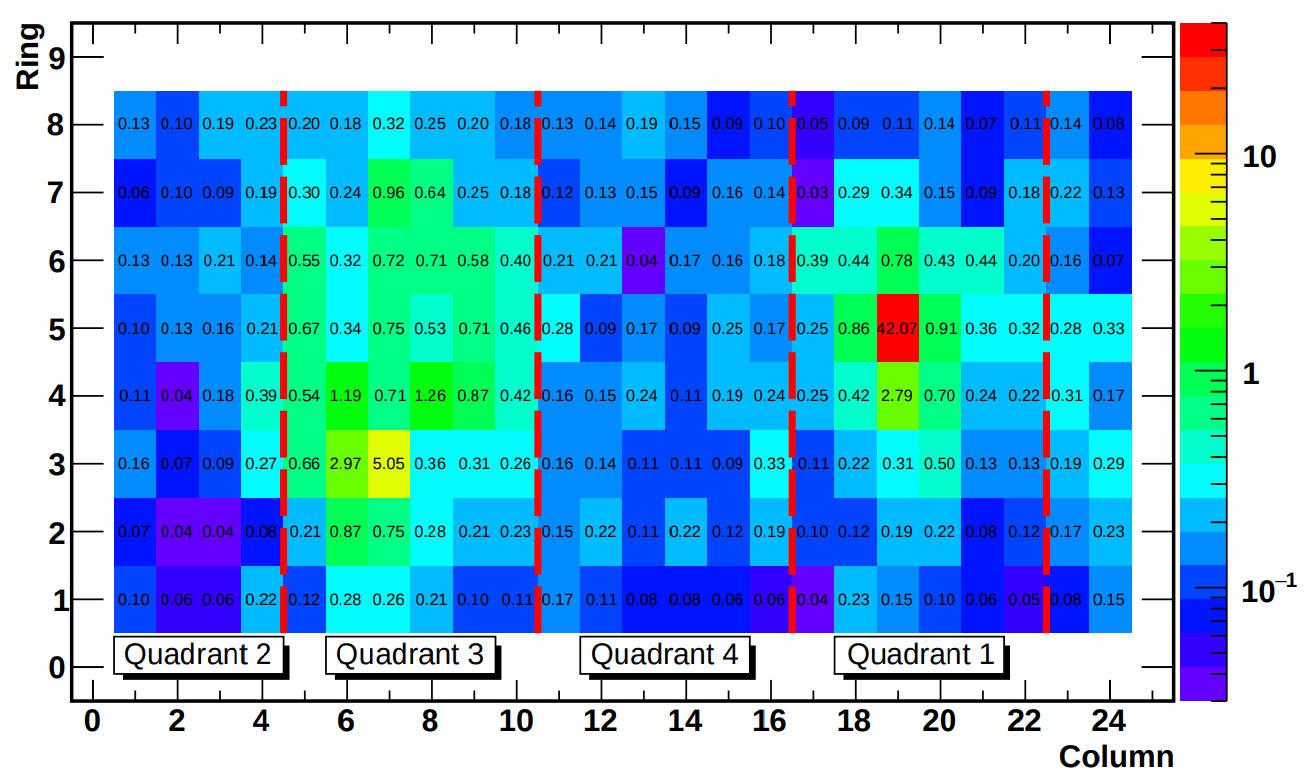
\includegraphics[width=\textwidth]{Backgrounds/Flasher/example_event.png}
  \caption{PMT charge distribution of a flasher candidate, illustrating the division of the AD into four azimuthal quadrants, with Quadrant 1 being centered around the PMT with the highest charge. From \cite{An_2017}.}
  \label{fig:flasher_example}
\end{figure}

\begin{figure}[h]
  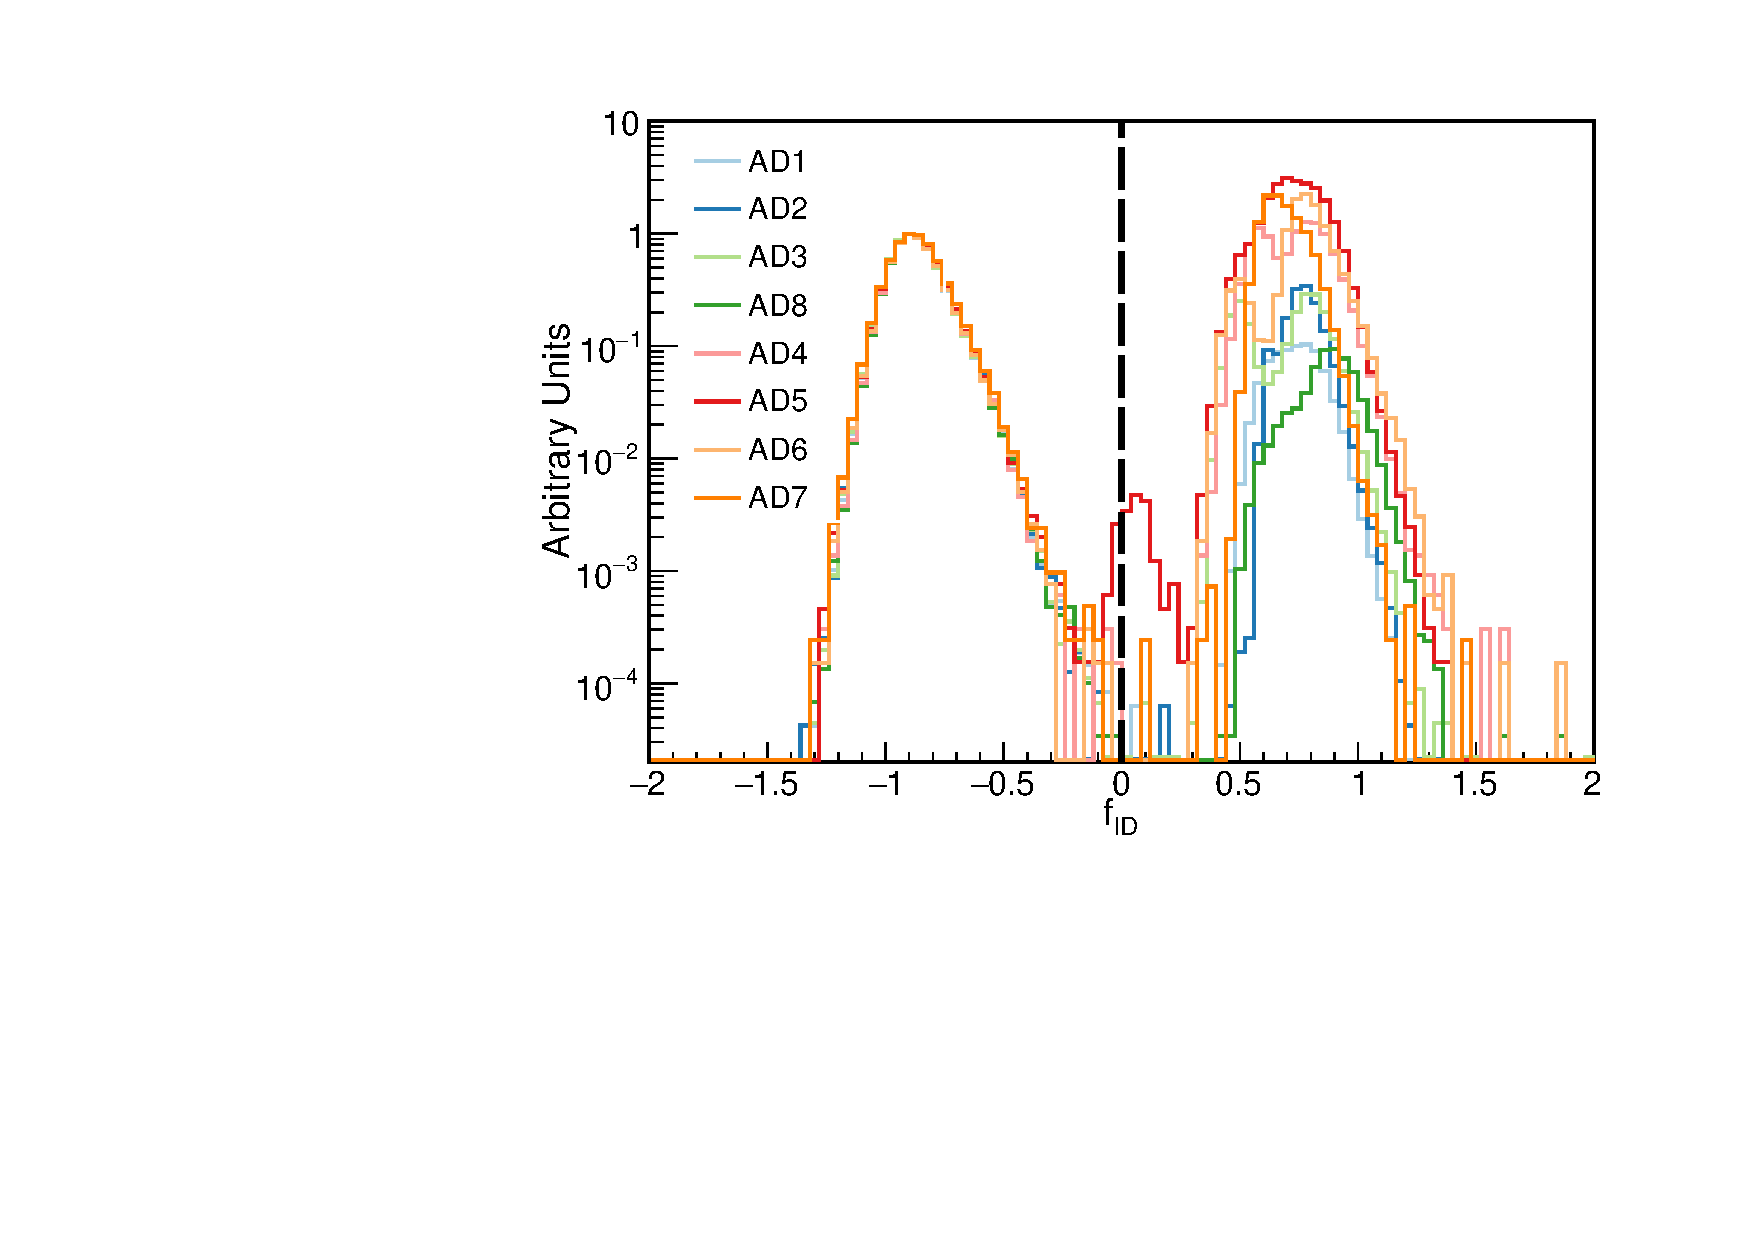
\includegraphics[scale=0.5]{Backgrounds/evt_flasherFID_Delayed.pdf}
  \caption{Distribution of the flasher discriminator $\fID$ for the delayed triggers of IBD candidates. The tagged flashers ($\fID > 0$) are cleanly separated from physics signals, with the exception of a single flasher in AD5 which leaked into the signal region (leading to a slight increase in the singles rate). In all ADs, there is essentially no signal lost. From \cite{An_2017}.}
  \label{fig:fID_dist}
\end{figure}

Even further flasher reduction can be achieved by incorporating timing information. To capture the broadening of the time distribution shown by flashers, we use the variable(s) $f_{\mathrm{t}1}$ ($f_{\mathrm{t}2}$), defined as the ratio of the number of hits in the first 200 (150)~ns of the signal, over the number of hits in the first 400~ns. The discriminator $\fPSD$ is then defined as
\begin{equation}
  \fPSD = \log_{10} [4 \cdot (1 - f_{\mathrm{t}1})^2 + 1.8 \cdot (1 - f_{\mathrm{t}2})^2].
\end{equation}
By requiring both $\fID < 0$ and $\fPSD < 0$, we eliminate virtually all 8" PMT flashers from the analysis.

However, in addition to the 192 8" PMTs, there are six 2" PMTs located at the top and bottom of each AD along the calibration axes, and these can also flash. Such events were easily identified as those in which any 2" PMT saw an extreme amount of charge, with a cut of 100 PE providing essentially perfect separation between 2" PMT flashers and other events.

The exact efficiency of these cuts (i.e., the rejection factor for flashers), is unimportant, as long as it is high enough.\footnote{According to \cite{SideBySide}, the efficiency is greater than $99.99\%$.} Any residual flashers will automatically be counted in the singles rate, and thus so will their contribution to the accidental background rate.\footnote{There is a small second-order correction due to the fact that an accidental cannot be formed by two flashers in the same PMT, given that it takes on the order of a second for a PMT to ``recharge'' after flashing. However, this correction is negigible given the extremely low rate of residual flashers.} As shown in \autoref{fig:fID_dist}, the rejection factor (and hence the purity of the IBD sample, with respect to flashers) is very nearly 100\% in all ADs, with the minor exception of AD5, where the small contribution of unrejected flashers will, in any case, be removed during the subtraction of the accidental background spectrum.

Compared to the efficiency, it \emph{is} important to study the signal inefficiency, i.e. the probability of improperly rejecting an IBD prompt or delayed trigger. If this inefficiency differs significantly among the ADs, it could bias the oscillation result.
% The inefficiency was estimated \cite{xinFlasherEff1,xinFlasherEff2} by taking a sample of IBD-like events (without the flasher cut), and making a 2D histogram of $(f_{\mathrm{prompt}},f_{\mathrm{delayed}})$, where $f$ is $\fID$ or $\fPSD$. The IBD-like sample consists of a small number of accidentals that contain a flasher (or two), and a much larger number of flasher-free pairs (including true IBDs, accidentals, and correlated backgrounds). The use of IBD-like events has the effect of diluting the presence of flashers in the sample, since a coincident pair is much more likely to come from an IBD than an accidental (which furthermore is more likely to have two physical singles rather than a flasher). The inefficiency was then determined by the degree to which the flasher-free ``blob'' extended into the regions rejected by the discriminator. These studies found that $\fID$ and $\fPSD$ each introduce a maximum inefficiency of 0.02\%, with uncertainties of 0.01\% correlated and 0.01\% uncorrelated.
%% From these studies, the efficiency of the flasher cut (when applied to true IBDs) was determined to be 99.98\% $\pm$ $0.01\%$ (correlated) $\pm$ $0.01\%$ (uncorrelated) \cite{An_2017}.
The inefficiency was estimated \cite{patrickFlashers} using a $\sim$600-day sample of IBD-like events (without any flasher cuts). For each of the three flasher discriminators (2", $\fID$, and $\fPSD$), a 2D histogram was constructed of its values for the prompt and delayed events. These histograms indicated that essentially all rejected IBDs had a flasher-like prompt (but not delayed) trigger. Accordingly, 1D histograms were then constructed of the discriminators of the prompt triggers for all pairs that lacked a flasher-like delayed trigger. Near the region of overlap between the IBD and flasher distributions, the true IBD distribution was fit (to both exponential and Gaussian functions) and extrapolated in order to estimate the fraction within the rejection region (\autoref{fig:flasher_fID_extrap}). Systematic uncertainties were determined by varying the fit range and function. These results were then cross-checked by exploiting the different prompt-delayed time correlations of the two event classes, giving an independent breakdown of the total distribution into its IBD and flasher components (\autoref{fig:flasher_fID_time}). The total inefficiency was found to be $0.039\% \pm 0.006\%$, as summarized in \autoref{tab:flasher_ineff}. AD-to-AD variations lay within this uncertainty band.

\begin{figure}[ht]
  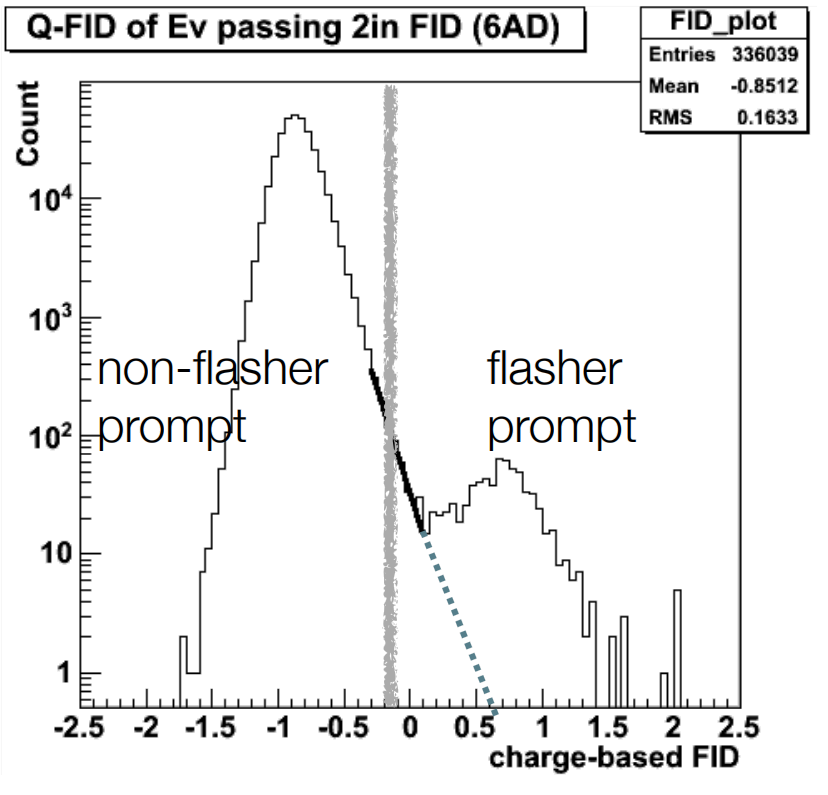
\includegraphics[width=0.5\textwidth]{Backgrounds/Flasher/ineff_fID_extrap.png}
  \caption{The prompt $\fID$ distribution of IBD-like events for which the delayed trigger is \emph{not} flasher-like (as determined by $\fID$). The true IBD component is fit and extrapolated in order to determine the inefficiency of the cut. From \cite{patrickFlashers}.}
  \label{fig:flasher_fID_extrap}
\end{figure}

\begin{figure}[ht]
  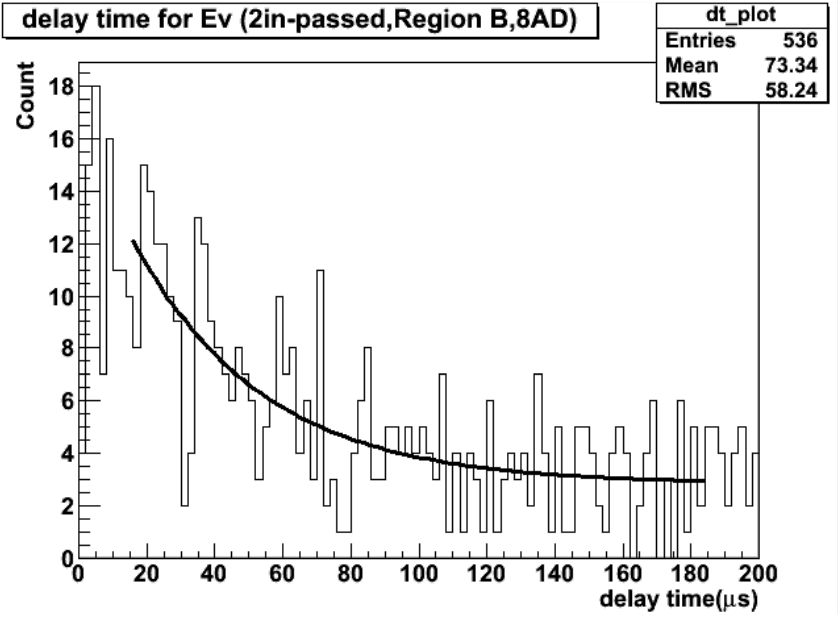
\includegraphics[width=0.5\textwidth]{Backgrounds/Flasher/ineff_fID_time.png}
  \caption{The prompt-delayed time difference of IBD-like events for which the delayed trigger is \emph{not} flasher-like (as determined by $\fID$). The true IBD component follows an exponential distribution, while the flasher component is flat. A fit is performed in order to quantify the two components. From \cite{patrickFlashers}.}
  \label{fig:flasher_fID_time}
\end{figure}

\begin{table}[ht]
  \begin{tabular}{lc}
    \toprule
    Cut & Inefficiency (\%) \\
    \midrule
    2" PMT  & $0.000 \pm 0.000$ \\
    $\fID$  & $0.023 \pm 0.004$ \\
    $\fPSD$ & $0.016 \pm 0.002$ \\
    \midrule
    Total & $0.039 \pm 0.006$ \\
    \bottomrule
  \end{tabular}
  \caption{Inefficiencies of the flasher cuts \cite{patrickFlashers}. For true IBDs, the distributions of the three discriminator were assumed to be uncorrelated, so that the total inefficiency was determined as the sum of the three. The systematic uncertainties were conservatively assumed to be fully correlated, and were thus added linearly rather than in quadrature.}
  \label{tab:flasher_ineff}
\end{table}


% We use both cuts in our analysis. Given that the two cuts are based on different information (charge and time), we assume that our estimated inefficiency is 0.04\%, with an uncertainty of 0.02\% correlated and 0.02\% uncorrelated.

% YYY show 2D plot of ellipse cut from doc-7143.

\section{Accidental coincidences}
\label{sec:accbkg}

IBD-like pairs can be formed when two uncorrelated triggers (\emph{singles}) ``accidentally'' occur closely together in time. Given that the prompt-like singles rate (after flasher rejection) is approximately 50~Hz in each AD,\footnote{Meanwhile, the delayed-like singles rate ranges from $\sim$0.001~Hz at the far site to $\sim$0.1~Hz at the near sites; this is still large enough to provide ample statistics from Daya Bay's multi-year dataset.} the characteristics of singles (and thus of accidentals) can be measured with extremely high statistical precision. Once the rates of prompt-like and delayed-like singles have been determined, the accidentals rate can be calculated via a straightforward application of Poisson statistics. This procedure is detailed in \autoref{sec:accratecalc}. The spectrum, meanwhile, is equal to that of the singles sample, whose extraction is described in \autoref{sec:selSingles}.

\begin{comment}
As previously stated, the accidental background can be straightforwardly measured based on the characteristics of singles events. The singles spectrum is first measured by searching for prompt-like events that satisfy the usual muon vetos but are separated from other prompt-like events by at least 400~$\mu$s. The total integral of this spectrum gives the prompt-like rate $R_p$, while the integral above 6~MeV gives the delayed-like rate $R_d$. The accidental background rate is then simply
\[ R_\mathrm{acc} = R_d(1 - e^{-R_p\Delta t})e^{-2R_p\Delta t}, \] where the factor in parentheses is the probability for a prompt-like single to fall within the $\Delta t$~=~200~$\mu$s preceding a delayed-like single, and the final factor is the probability that the event is \emph{not} rejected by the decoupled multiplicity cut, which disallows any additional prompt-like single in the 400~$\mu$s preceding the delayed event. Once the rate has been determined this way, the spectrum is trivial: It is simply the singles spectrum itself.
\end{comment}

\begin{comment}
  Mention IHEP's cross-check, and the additional uncertainty stemming from the difference between it and the nominal result?
\end{comment}

\section{Cosmogenic $^9$Li/$^8$He}
\label{sec:bkgCosmo}

\newcommand\linine{$^9$Li}

The dominant correlated background for Daya Bay comes from the isotopes $^9$Li and $^8$He, which are produced as spallation products of carbon when energetic muons traverse the AD. These two isotopes have relatively long lifetimes of 257~ms for $^9$Li and 172~ms for $^8$He \cite{ENDF} (see \autoref{tab:bkgLi9He8Props}); thus, while the majority of them will decay within the O(1~s) veto window that follows showering muons, a non-negligible fraction will survive past it. As shown in \autoref{fig:li9he8_decays}, when one of these isotopes undergoes beta decay into the relevant excited states of the daughter nucleus, the daughter will immediately emit a neutron (and, in the case of $^9$Li, will further disintegrate into two alpha particles). The relevant $\beta$ decay endpoints extend up to 12~MeV, placing these decays squarely within the IBD prompt-energy region. The combination of this $\beta$ decay and the subsequent nGd capture produces the characteristic double-coincidence signature of an IBD event. In what follows, we will collectively refer to these two isotopes as $^9$Li, given that it is believed to be the predominant of the two. (For instance, the KamLAND collaboration's FLUKA simulations \cite{KamLAND_cosmo} indicated a 10:1 ratio of $^9$Li to $^8$He production.\label{par:kamland_he8}\footnote{Given KamLAND's higher $\langle E_\mu \rangle$ of 260~GeV, compared to Daya Bay's $\sim$50 (100) GeV at the near (far) site(s), KamLAND's measured ratio of $^9$Li to $^8$He may not be completely representative, but in the absence of additional data, it is an acceptable starting point. In practice, as discussed later, we use a nominal (and somewhat arbitrary) $^8$He fraction of 5.5\%, with other values trialed as part of the overall uncertainty estimation.}) Later we will propagate the uncertainty on this ratio into the background estimation. 

\begin{table}[h]
  \begin{tabular}{lccc}
    \toprule
    Isotope & Lifetime (ms) & $\beta$ decay endpoint (MeV) & Final products \\
    \midrule
    $^9$Li & 257.2 & 11.17 & $e^-$ + $\alpha$ + $\alpha$ + n (+ $\nuebar$)\\
    $^8$He & 171.6 & 7.44 & $e^-$ + $^7$Li  + $\gamma$ + n (+ $\nuebar$)\\
    \bottomrule
  \end{tabular}
  \caption{Properties of the cosmogenic isotopes $^9$Li and $^8$He \cite{ENDF}. The quoted $\beta$ decay endpoint is the endpoint of the highest-energy transition \emph{that produces a final neutron}.}
  \label{tab:bkgLi9He8Props}
\end{table}

\begin{figure}[h]
  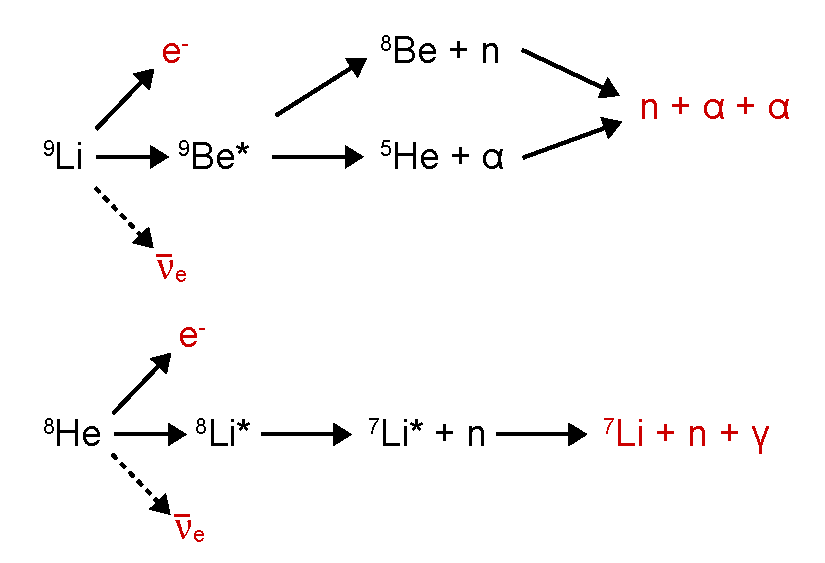
\includegraphics[scale=0.75]{Backgrounds/li9he8_decays.pdf}
  \caption{Decay cascades of $^9$Li and $^8$He with excited daughter nuclei after $\beta$ decays. Final products are highlighted in red. Extended from \cite{pedroLi9Spec2}.}
  \label{fig:li9he8_decays}
\end{figure}

Although at Daya Bay there is no feasible way of distinguishing \linine\ decays from IBDs at the level of individual events, it is still possible to statistically estimate the total \linine\ rate by exploiting the correlation in time between \linine\ events and preceding muons. To see this, let the muon rate be denoted by $R_\mu$, and the \linine\ livetime by $\tau$. Since IBD events are uncorrelated with muons, the time between an IBD and the most recent preceding muon is given, according to Poisson statistics, by the probability density function (PDF)
\begin{equation}
  \label{eq:cosmoBkgPdfIbd}
  f_{\mathrm{IBD}}(t) = R_\mu e^{-R_\mu t}.
\end{equation}
Meanwhile, a \linine\ decay is correlated in time with the parent muon:
\begin{equation}
  \label{eq:cosmoBkgPdfLiProd}
  f_{\mathrm{Li,\,Parent}}(t) = \frac{1}{\tau} e^{-t/\tau}.
\end{equation}
However, in the time between a muon shower and an associated \linine\ decay, additional muons may be detected, and these may closely resemble the true parent muon. As such, the quantity that we can reliably measure is not the time between the \linine\ decay and the parent muon, but (as with IBDs) the time between the decay and the \emph{last} muon. This detail has the effect of modifying the time constant in \autoref{eq:cosmoBkgPdfLiProd}. To derive this modification, let us consider a \linine\ event with a time-to-last-muon of $t$. Either the last muon was the parent muon, or it wasn't. Defining our time axis with the decay at the origin, these two possibilities can be stated quantitatively as:
\begin{enumerate}
\item The parent muon occured at time $-t$, with no intervening uncorrelated muons, or
\item The parent muon occured at some (unknown) time prior to $-t$, and the most recent uncorrelated muon occured at $-t$.
\end{enumerate}
The parent muon's time PDF is given by \autoref{eq:cosmoBkgPdfLiProd}, and that of the most recent uncorrelated muon by \autoref{eq:cosmoBkgPdfIbd}. Meanwhile, the Poisson probability of observing zero uncorrelated muons in a time window of $t$ is given by $e^{-R_\mu t}$. Thus, letting $P_1$ and $P_2$ be the probabilities\footnote{Here we will say ``probability'' when we really mean ``probability density''.} of the two cases above, we have
\begin{align*}
  P_1 = \frac{1}{\tau} e^{-t/\tau} \cdot e^{-R_\mu t} = \frac{1}{\tau}e^{-(R_\mu + 1/\tau)t}
\end{align*}
and
\begin{align*}
  P_2 = \int_t^\infty \frac{1}{\tau}e^{-t'/\tau}\,dt' \cdot R_\mu e^{-R_\mu t} = e^{-t/\tau} \cdot R_\mu e^{-R_\mu t} = R_\mu e^{-(R_\mu + 1/\tau)t}.
\end{align*}
Letting
\begin{equation}
  \lambda = R_\mu + 1/\tau,
\end{equation}
we finally add $P_1$ and $P_2$ to obtain the PDF of time-to-last-muon for \linine\ decays:
\begin{equation}
  \label{eq:cosmoBkgPdfLi}
  f_{\mathrm{Li}}(t) = \lambda e^{-\lambda t}.
\end{equation}

Comparing \autoref{eq:cosmoBkgPdfLi} and \autoref{eq:cosmoBkgPdfIbd}, we see that, if $\lambda$ is sufficiently different from $R_\mu$ (in other words, if $R_\mu$ is sufficiently small relative to $1/\tau$), then there will be a measurable difference between the time-to-last-muon PDFs of \linine\ and IBD events. In this case, the separate event counts can be obtained by constructing a histogram of time-to-last-muon from a mixed sample of IBDs and \linine\ events. This histogram can then be fit to a weighted sum of \autoref{eq:cosmoBkgPdfLi} and \autoref{eq:cosmoBkgPdfIbd}, with the weights (as detemined by the fit) corresponding to the number of events in the two categories:
\begin{equation}
  f(t) = N_{\mathrm{Bkg}} \lambda e^{-\lambda t} + N_{\mathrm{IBD}} R_\mu e^{-R_\mu t}.
\end{equation}

If the fit is allowed to extend down to $t$ of a couple dozen ms, an additional correlated component must be considered resulting from accidental double coincidences of $^{12}$B and/or $^{12}$N decays. These two isotopes, with respective lifetimes of 29 and 16~ms \cite{ENDF}, and $\beta^\pm$ endpoints of 13.7 and 16.3~MeV \cite{ENDF}, can be produced multiple times by a single muon shower, and their decays extend well into the delayed-energy region. Their double coincidences are already considered as part of the accidental background estimation\footnote{There is some bias owing to the fact that the prompt and delayed $^{12}$B/$^{12}$N are not uncorrelated in time (as assumed in the accidentals calculation), but are in fact correlated by virtue of their usually coming from the same parent muon. However, the rate of such events is extremely low (relative to the total accidentals rate), as can be seen in the fits shown later in this chapter, so there is no need to attempt a correction to the accidentals rate.}, so we are not concerned with measuring them here as a separate background; however, they do distort the time-to-last-muon histogram at low times, and thus they must be considered in order to extract the \linine\ component accurately. Past fits \cite{NonlinearityPaper} to the spectrum of muon-correlated singles have indicated that $^{12}$B is by far the dominant of these isotopes (comprising some 97\% of the events), so in what follows we treat it as the only one of relevance.

When fitting the time-to-last-muon for the $^{12}$B double coincidences (BB events, for short), the time constant must be considered carefully. We first consider the time to the \emph{parent} muon, rather than to the \emph{last} muon. For the single $^{12}$B events, the corresponding time constant is simply the $^{12}$B lifetime $\tau_{\mathrm{B}}$.  However, if a muon produces two $^{12}$B nuclei, then a timespan of $t$ will correspond to an $e^{-t/\tau_{\mathrm{B}}}$ survival probability of one nucleus, and likewise for the other. The observation of one decay, of either nucleus, constitutues an observation of the whole pair, since we are recording the time between muons and the \emph{prompt} event in an IBD candidate. The probability of not observing the pair, then, is the probability of seeing \emph{neither} nucleus decay, which is $(e^{-t/\tau_{\mathrm{B}}})^2 = e^{-t/(\tau_{\mathrm{B}}/2)}$. That is, the time constant for the BB time-to-parent-muon distribution is $\tau_{\mathrm{B}}/2$. For the time to the \emph{last} muon, rather than the parent, the arguments preceding \autoref{eq:cosmoBkgPdfLi} then imply a rate constant of $\lambda_{\mathrm{BB}} = R_\mu + 2/\tau_{\mathrm{B}}$.
\begin{comment}
\footnote{We neglect the possibility of only seeing \emph{one} of the nuclei decay, since the IBD coincidence cut of \us{200} is far shorter than the $^{12}$B lifetime of 29~ms, and therefore, the observation of one decay effectively \emph{implies} the observation of the other.}

 As such, the time constant for BB events is $\tau_{\mathrm{B}}/2$. (I'm not sure I buy this. We are \emph{assuming} that the two decays occur within 200~us of each other, and the probability of seeing them both is basically equivalent to the probability of seeing the first, and the time-to-last-muon PDF for the first just has the time constant of $\tau$. Where the time constant \emph{does} get halved is if we consider a muon that produces two nuclei and we want the probability of seeing none i.e. the time to the next decay.)
\end{comment}

\begin{comment}
  YYY our code has the 12B half-life (20 ms) listed as the lifetime (should be 29 ms). This further exacerbates the use of the mistaken(???) factor of 2??? In total our time constant has been off by a factor of 3 (well, plus the Rmu part)
\end{comment}

To finish deriving the full expression used in fitting the time to last muon, we simply add a factor $r$ corresponding to the $^8$He fraction, giving
\begin{equation}
  \label{eq:bkgLi9FullExpr}
  f(t) = N_{\mathrm{Bkg}} \left[ (1-r)\lambda_{\mathrm{Li}} e^{-\lambda_{\mathrm{Li}} t} + r\lambda_{\mathrm{He}} e^{-\lambda_{\mathrm{He}} t }\right] + N_{\mathrm{BB}} \lambda_{\mathrm{BB}} e^{-\lambda_{\mathrm{BB}} t} + N_{\mathrm{IBD}} R_\mu e^{-R_\mu t},
\end{equation}
where
\begin{align*}
  \lambda_{\mathrm{Li}} &= R_\mu + 1/\tau_{\mathrm{Li}} \\
  \lambda_{\mathrm{He}} &= R_\mu + 1/\tau_{\mathrm{He}} \\
  \lambda_{\mathrm{BB}} &= R_\mu + 2/\tau_{\mathrm{B}}.
\end{align*}

Although this method is simple in theory, a significant challenge arises from the fact that a minimum muon energy must be defined when calculating the time between each event and its most recent preceding muon. If this cut is too low, then the time between muons will be comparable to (or smaller than) the \linine\ livetime, and with finite statistics, it will be difficult to reliably distringuish between the two components in the fit. Conversely, if the muon cut is too high, then some fraction of \linine-producing muons will be discarded, and those \linine\ events will not appear to be muon-correlated, leading to an underestimation of the rate.

This issue is mitigated somewhat by the fact that low-energy muons produce a relatively small portion of the total \linine\ rate.\footnote{More precisely, at the near (far) sites, some 80\% (90\%) of the $^9$Li in the IBD sample comes from muons of visible energy above 1~GeV. This can be deduced from the results shown in \autoref{tab:bkgLi9Rates} (where 1~GeV $\sim$ 160,000 photoelectrons).}
% Note: See /home/mkramer/apps/spacemacs/.emacs.d/.cache/junk/2020/11/28-li9frac.jl
However, an accurate assessment must still attempt to quantify the contribution from low-energy muon events. To enhance the \linine\ signal in the fit, either the muon sample or the \linine\ candidate sample (or both) must be somewhat purified. Purifying the muon sample will enhance the difference in time constants between the $^9$Li and IBD components, while purifying the $^9$Li sample will enhance the difference in amplitudes. We use both methods in what follows.

For the muon sample, the goal is to remove muons that are unlikely to produce a \linine\ event. This will reduce the muon rate $R_\mu$, thus increasing the difference between the time constants of the fit components. However, the cost of this \emph{muon reduction} is that some fraction of \linine-producing muons will be discarded. The associated \linine\ events will have a time-to-last-muon rate constant of $R_\mu$ rather than $\lambda$, so they will not contribute to the measured \linine\ rate, leading to an inefficiency (and corresponding uncertainty) in the total rate estimate. Here, muon reduction is achieved by using \emph{neutron tagging}, in which we only consider those muons for which a neutron capture candidate is observed in the immediate aftermath. Given the sizable uncertainty on the efficiency of the tagging, this method is only used where absolutely necessary, i.e., in the bin of the lowest muon energy. The details are discussed later.

As for increasing the purity of the \linine\ sample, the method used here is simply to apply a cut on the prompt energy. As can be seen by comparing \autoref{fig:li9_spec} to \autoref{fig:selPromptSpec}, the \linine\ and IBD spectra differ substantially, with the former being much harder. As such, a higher prompt-energy cut will increase the ratio of \linine\ to IBD events. This benefit, however, must be weighed against the loss in the total statistics arising from an aggressive prompt-energy cut. Here, heuristically chosen cuts are used in order to obtain acceptable fits. As will be detailed later, more aggressive cuts are used in the near hall (where the IBD ``background'' fraction is larger) and for lower muon energies (where a greater \linine\ purity is needed due to the proximity of $\lambda$ to $R_\mu$). These prompt cuts, together with neutron tagging (for low muon energies), enable the \linine\ fit to be performed for muon energies that extend all the way down to the ``AD muon'' threshold of 3,000~pe.

In the sections that follow, we describe the \linine\ rate estimation in detail, beginning with the selection of \linine\ candidates, followed by the muon selection, the fitting procedure, its results, the various selection efficiencies, and the error budget. Our method is a repeated and slightly modified version of the one described by Chris Marshall in \cite{ChrisLi9}, which in turn was based on a 2014 analysis performed by the author in \cite{MattLi9}.

\subsection{$^9$Li candidate selection}
\label{sec:bkgLi9Sel}

The $^9$Li selection is largely identical to the standard IBD selection, as described in \autoref{chap:selection}, but with two key differences: First, the prompt-energy cut is higher, as described above (although this cut is applied after the initial selection, for the sake of flexibility), and, secondly, the ``shower muon'' veto is disabled. That is, rather than vetoing for 0.4004~s after a muon of $>$300,000~pe (as in our nominal IBD selection), only the ``AD muon'' veto of 1.4~ms is applied. This is necessary because the shower veto would otherwise remove a large fraction of the $^9$Li events, greatly reducing the already-limited statistics of the sample. More precisely, for a given $^9$Li event produced by a shower muon, the probability of its falling within the veto window is
\begin{equation}
  \label{eq:bkgLi9VetoProb}
  1 - \exp\left( - \frac{400.4}{257} \right) \approx 80\%,
\end{equation}
where the numerator is the veto time and the denominator is the $^9$Li lifetime (in milliseconds, in both cases). As shown in \autoref{tab:bkgLi9Rates}, some 90\% of $^9$Li events are produced by shower muons. Multiplying this percentage by that from \autoref{eq:bkgLi9VetoProb} implies that some 70\% of $^9$Li events would be lost if the shower veto were applied. A similar argument applies for $^8$He.

When producing the final \linine\ rate estimation, we must correct for the efficiency of this modified muon veto. Using the muon toy MC described in \autoref{sec:cutVaryMuVetoEff}, these efficiencies were determined to be 87\%, 90\%, and 99\% in EH1, EH2, and EH3, respectively. (Compare to 82\%, 85\%, and 98\% for the standard muon veto.)

% YYY the Li9 rates, as I've been using them so far, are calculated assuming the efficiencies of the standard muon veto, rather than the modified one. I've corrected the constants in Li9Calc accordingly, but need to rerun the calculation and update the plots etc. ... I think I fixed it in yolo4 and oct20v3?

\subsection{Muon selection}
\label{sec:bkgLi9MuonSel}

For the purposes of applying the muon veto and constructing the time-to-last-muon distributions, we use the muon tree generated by the Daya Bay software framework (\texttt{NuWa}) during data production, as discussed in \autoref{sec:selProd}. In this tree, muons that trigger multiple detectors are merged into a single muon, and prompt retriggers are discarded. This represents a minor difference from our IBD selection, where retriggers are \emph{not} discarded, leading to a slight reduction in our muon veto efficiency compared to what we'd obtain from using the \texttt{NuWa} muon tree. (This difference is correctly accounted for in the summation of veto windows, and thus there is no resulting bias.) For the $^9$Li analysis, the removal of retriggers helps to prevent any biasing of the time constant for $^9$Li events. The \texttt{NuWa} muon selection's cuts are designed to be looser than any conceivable muon definition used in a physics analysis (which would in turn select a subset of \texttt{NuWa's} ``muons''). Accordingly, they are as follows:

\begin{itemize}
\item A trigger in the inner (outer) water pool, with at least 6 (8) fired PMTs, is tagged as a WP muon.
\item A trigger in an AD of more than 3000 photoelectrons is tagged as an AD muon.
\item Tagged muons that occur within a 300~ns window are merged into a single muon (with the WP hit counts and AD charges individually stored), with the timestamp taken to be the time of the earliest trigger.
\item Any subsequent ``muons'' that occur within 10~\us\ are deemed to be retriggers and are thus discarded.
\end{itemize}

During the $^9$Li selection, a given muon object will result in the 1.4~ms AD muon veto if the object contains an AD muon for the detector in question. If not, but if there is a IWP or OWP muon present with \emph{more than 12 hit PMTs}, then the 600-\us\ WP muon veto is applied instead.

If a $^9$Li candidate is found, then all preceding muons within a 10-second window are stored in an array specific to that candidate. This array can then be looped over when constructing the time-to-last-muon histogram, skipping over muons outside of a chosen energy range until the most recent one within the energy range is found.

\subsubsection{Neutron tagging}
\label{sec:bkgLi9NeuTag}

In order to enable the neutron tagging technique (as needed for calculating the rate of $^9$Li produced by low-energy muons), an additional flag is stored for each muon, indicating whether the muon occurred in coincidence with a neutron capture candidate. Specifically, the neutron tag is applied if any trigger ranging from 1.8 to 12~MeV
% (YYY why is it 18~MeV in the code?)
occurs between 20 and 200~\us\ after the muon. Although these cuts are heuristic, they are reasonable in principle: The energy range is wide enough to include captures on both gadolinium and hydrogen, and the time window includes most of the Gd captures and a decent fraction of H captures, while avoiding spurious signals that can arise from retriggers occurring in the first dozen or so \us\ after a muon.

The primary challenge in using the neutron tagging technique is accounting for the efficiency of the tagging. That is, what percentage of $^9$Li-producing AD muons (within a specified energy range) will be neutron-tagged? For sufficiently high-energy muons (roughly above 160,000 photoelectrons), the $^9$Li rate can be measured both with and without neutron tagging, and thus the efficiency can be extracted directly. However, for muons below 160,000~pe (where neutron tagging is unavoidable), this is not possible, and the efficiency must be extrapolated. We discuss this efficiency, and its uncertainty, in \autoref{sec:bkgLi9NeuTagEff}.
% In \cite{WeiLi9}, the efficiency is measured across a range of muon energies, and found to range from $\sim$90\% for muons above 1.8~GeV ($\sim$290,000~p.e.), down to $\sim$60\% for muons of 1.0--2.5~GeV (1.6--4e5~p.e.). For the sake of analysis, we thus assume a neutron tagging efficiency of 60\% (YYY need to fix this in Li9Calc and generate new results!!!), and apply a corresponding relative uncertainty of 45\% to the $^9$Li rate for muons below 160,000~p.e.

\subsection{Time-to-last-muon fit}
\label{sec:bkgLi9HistoFit}

Once a sample of $^9$Li candidates has been collected, along with the history of prior muons for each such candidate, the next step is to construct the histogram of times since the most recent muon (within a given muon energy range). We use a histogram spanning from 2~ms to 1~s, with a nominal binning consisting of 24 variable-width bins. The lowest bin covers 2 to 20~ms; the next four bins (up to 100~ms) are 20-ms-wide; the next four (up to 0.5~s) are 0.1-s-wide; the next six (up to 2~s) are 0.25-s-wide; the next two (up to 3~s) are 0.5-s-wide; and the final seven are 1-s-wide. This variable binning scheme captures the fine structure at low times while keeping the number of bins at a manageable level. Later we discuss the systematic uncertainty arising from variation of the binning.

For each hall, three histograms were constructed, corresponding to three muon visible energy ranges of $<$160,000, 160,000-300,000, and $>$300,000~pe.\footnote{As detailed in \autoref{chap:cutVary}, we later vary the definitions of these ranges in order to capture the dependence of the final $^9$Li rate on the muon energy used in the definition of the shower muon veto. The ranges described here apply to the shower veto used in the nominal IBD selection.} Different cuts are used in the three ranges, as detailed in \autoref{tab:bkgLi9Cuts}. To fill each histogram, we loop over all $^9$Li candidates for the hall in question, and if the candidate is accepted by the prompt-energy cut, we then find the most recent preceding muon (within the specified energy range, and with a neutron tag when required). The time between the candidate and the muon is then used to fill the histogram.

\begin{table}[h]
  \centering
  \begin{tabular}{lccc}
    \toprule
    Hall & PE range ($\times10^3$) & Prompt cut (MeV) & Neutron tag? \\
    \midrule
    EH1/2  & 5-160   & 8.0 & Yes \\
           & 160-300 & 8.0 & No  \\
           & 300-inf & 3.5 & No  \\
    \midrule
    EH3  & 5-160   & 6.0 & Yes \\
         & 160-300 & 6.0 & No  \\
         & 300-inf & 3.5 & No  \\
    \bottomrule
  \end{tabular}
  \caption{Cuts used in constructing the three separate time-to-last-muon histograms for each hall.}
  \label{tab:bkgLi9Cuts}
\end{table}

After constructing the histogram, we fit it to \autoref{eq:bkgLi9FullExpr}. The results are shown in Figures~\ref{fig:li9_fits_eh1}--\ref{fig:li9_fits_eh3}. For the nominal result, we fix the $^8$He fraction $r$ to be 5.5\% (an inherited ``reasonable guess'', as discussed further in \autoref{sec:bkgLi9Spectrum}), and include the $^{12}$B component. Later we discuss the effects of varying the $^8$He fraction and the inclusion of $^{12}$B. The best-fit value of $N_{\mathrm{Bkg}}$, as determined by \texttt{MINUIT}, corresponds to the raw number of (muon-correlated) $^9$Li/$^8$He events present in the sample used for filling the histogram. As discussed in \cite{ChrisLi9}, the fit does not suffer from any appreciable correlation between $N_{\mathrm{Bkg}}$ and $N_{\mathrm{IBD}}$, as the latter is strongly constrained by the tail at high time-to-last-muon. This was verified in \cite{ChrisLi9} by hand-scanning the variation of $\chi^2$ as a function of $N_{\mathrm{Bkg}}$. Thus, \texttt{MINUIT's} reported statistical uncertainty on $N_{\mathrm{Bkg}}$ can be safely taken at face value and propagated into our final uncertainty. Our fit results are summarized in \autoref{tab:bkgLi9Rates}. As discussed further in \autoref{chap:cutVary}, the fit was also performed using alternative muon energy ranges, in order to characterize the dependence of the $^9$Li rate on the choice of shower-muon threshold.

\begin{figure}[ht]
  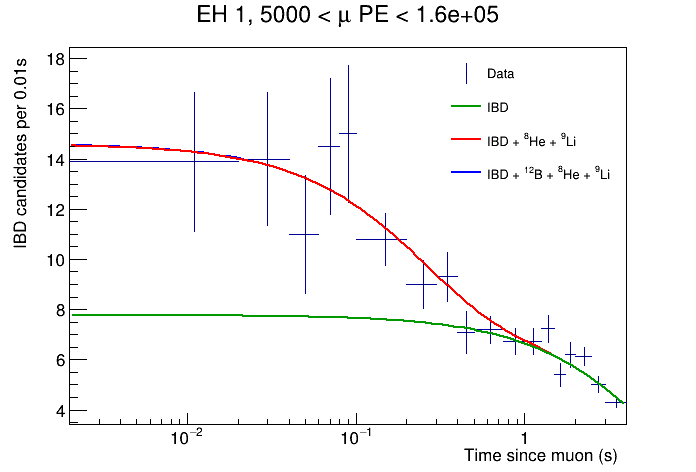
\includegraphics[width=0.5\linewidth]{Backgrounds/Li9/fits/EH1_range1_CV_logx.png} \\[0.5em]
  \begin{minipage}{0.5\textwidth}%
    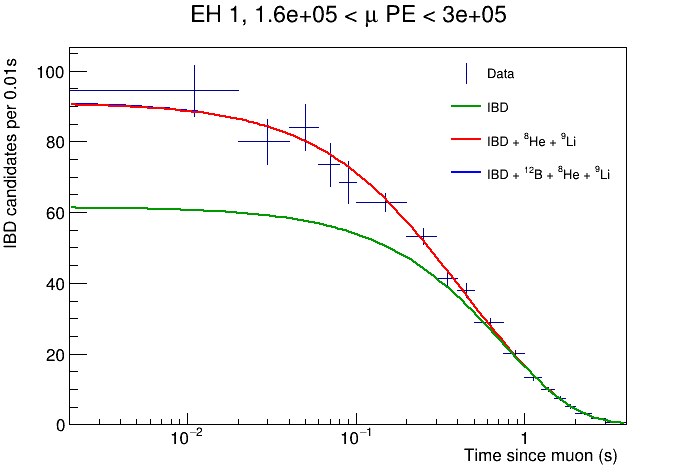
\includegraphics[width=\linewidth]{Backgrounds/Li9/fits/EH1_range2_CV_logx.png}%
  \end{minipage}%
  \begin{minipage}{0.5\textwidth}%
    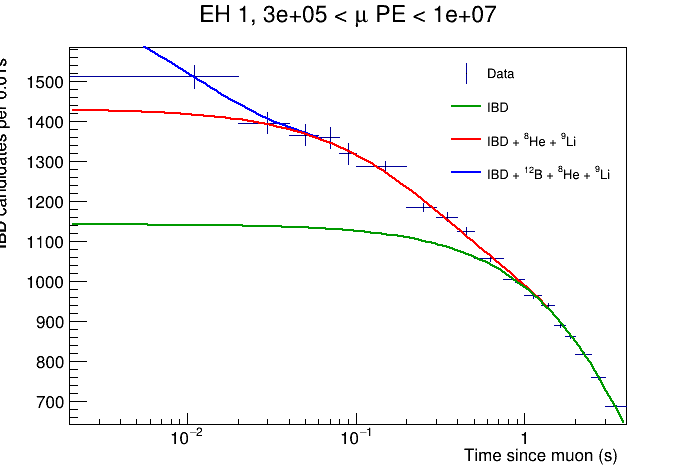
\includegraphics[width=\linewidth]{Backgrounds/Li9/fits/EH1_range3_CV_logx.png}%
  \end{minipage}%
  \caption{Time-to-last-muon fits for IBD-like events in EH1.}
  \label{fig:li9_fits_eh1}
\end{figure}

\begin{figure}[ht]
  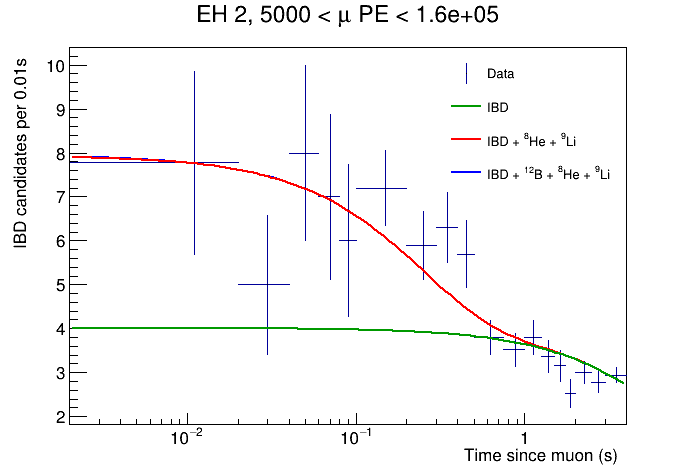
\includegraphics[width=0.5\linewidth]{Backgrounds/Li9/fits/EH2_range1_CV_logx.png} \\[0.5em]
  \begin{minipage}{0.5\textwidth}%
    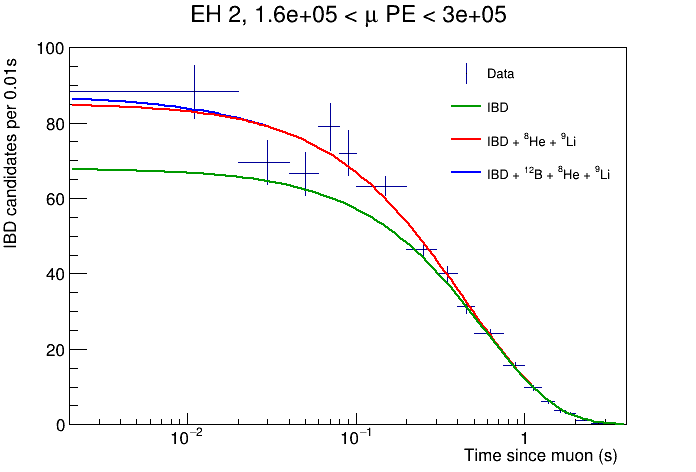
\includegraphics[width=\linewidth]{Backgrounds/Li9/fits/EH2_range2_CV_logx.png}%
  \end{minipage}%
  \begin{minipage}{0.5\textwidth}%
    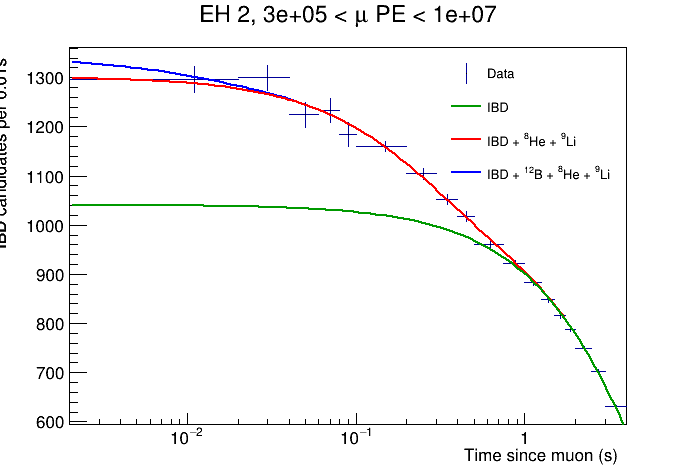
\includegraphics[width=\linewidth]{Backgrounds/Li9/fits/EH2_range3_CV_logx.png}%
  \end{minipage}%
  \caption{Time-to-last-muon fits for IBD-like events in EH2.}
  \label{fig:li9_fits_eh2}
\end{figure}

\begin{figure}[ht]
  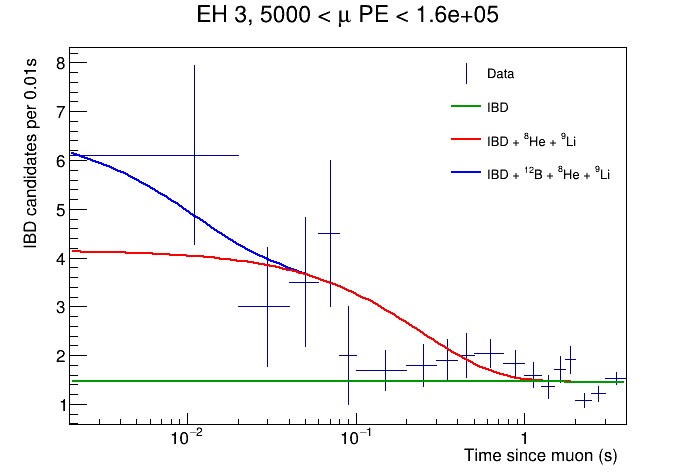
\includegraphics[width=0.5\linewidth]{Backgrounds/Li9/fits/EH3_range1_CV_logx.png} \\[0.5em]
  \begin{minipage}{0.5\textwidth}%
    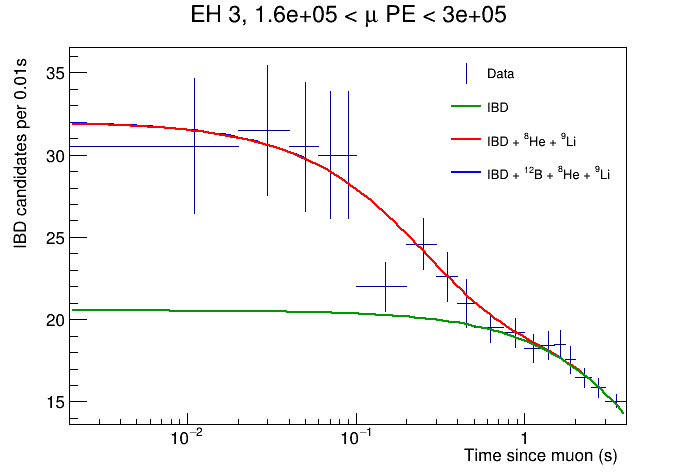
\includegraphics[width=\linewidth]{Backgrounds/Li9/fits/EH3_range2_CV_logx.png}%
  \end{minipage}%
  \begin{minipage}{0.5\textwidth}%
    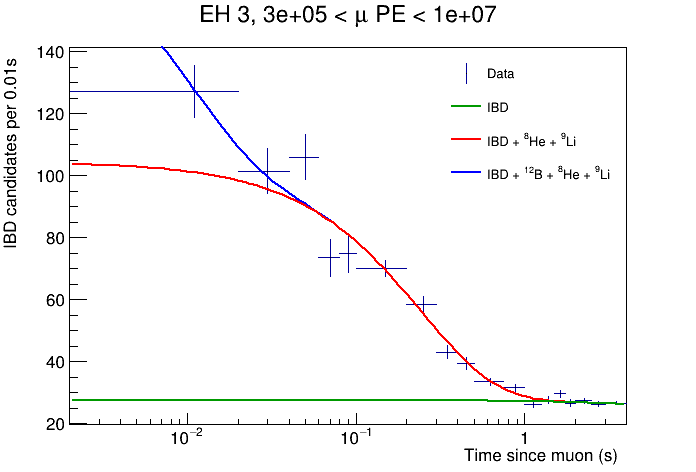
\includegraphics[width=\linewidth]{Backgrounds/Li9/fits/EH3_range3_CV_logx.png}%
  \end{minipage}%
  \caption{Time-to-last-muon fits for IBD-like events in EH3.}
  \label{fig:li9_fits_eh3}
\end{figure}

\begin{table}[h]
  \centering
  \begin{tabular}{lcc}
    \toprule
    Hall & PE range ($\times10^3$) & $N_{\mathrm{Bkg}}$ \\
    \midrule
    EH1  & Low (5-160)   & 164.0 $\pm$ 51.4 \\
         % & Mid (160-300) & 554.9 $\pm$ 0.2 \\
         & Mid (160-300) & 554.9 $\pm$ 200.5 \\
         & High (300-inf) & 6969.2 $\pm$ 675.4 \\
    \midrule
    EH2  & Low (5-160)   & 95.8 $\pm$ 27.4 \\
         % & Mid (160-300) & 301.7 $\pm$ 0.1 \\
         & Mid (160-300) & 301.7 $\pm$ 118.5 \\
         & High (300-inf) & 6282.7 $\pm$ 733.3 \\
    \midrule
    EH3  & Low (5-160)   & 66.8 $\pm$ 25.5 \\
         % & Mid (160-300) & 280.1 $\pm$ 67.5 \\
         & Mid (160-300) & 280.1 $\pm$ 89.4 \\
         & High (300-inf) & 1915.1 $\pm$ 182.4 \\
    \bottomrule
  \end{tabular}
  \caption{Measured number of $^9$Li+$^8$He events, as determined by the time-to-last-muon fit, for each hall and range of muon energies. Quoted errors are the statistical uncertainties reported by the fitter. No efficiency corrections have been applied.}
  \label{tab:bkgLi9Rates}
\end{table}
% NB: For mid-range, took relative errors from matt_li9_rates.txt (320k).

\subsection{Selection efficiencies and their uncertainties}
\label{sec:bkgLi9SelEffs}

\subsubsection{Prompt-energy cut}
\label{sec:bkgLi9PromptCutEff}

To determine the efficiences (and the corresponding uncertainties) of the prompt-energy cuts, we replicate the procedure developed in \cite{ChrisLi9}.\footnote{We deviate from \cite{ChrisLi9} in using a muon cut of 300,000~PE, rather than 400,000~PE, when selecting the $^9$Li-enriched sample used in the efficiency determination.} These efficiencies can simply be calculated by integrating the normalized $^9$Li spectrum (expressed in reconstructed energy) over the energies above each cut. The difficulty, however, lies in obtaining this spectrum. When subtracting the $^9$Li background from the spectrum of IBD candidates, we follow the tradition of using Ochoa's theoretical calculation of the spectrum, as described in \autoref{sec:bkgLi9Spectrum}. However, for the prompt-energy cut efficiencies, we extract the $^9$Li reconstructed spectrum directly from data.
% (TODO: Compare efficiencies from integrating Pedro's spectra.)
% We briefly describe his method here.

The spectrum extraction proceeds in two steps. First, a spectrum is obtained from a sample that is enriched in $^9$Li, and then a $^9$Li-deficient sample (consisting mainly of IBD ``background'') is acquired, rescaled, and subtracted from the $^9$Li-rich sample. This procedure produces a spectrum that contains very little contamination and can thereby give a reliable measurement of the prompt-energy cut efficiency.

To obtain the $^9$Li-rich sample, the $^9$Li candidates from all three halls were combined, and a subset was taken by selecting events that fell between 2 and 200~ms after a high-energy shower muon, defined here as a muon that produced more then 300,000 photoelectrons of visible energy. The time-to-last-muon fit of \autoref{eq:bkgLi9FullExpr} was then performed, giving the relative fraction of the sample comprised by \emph{shower-correlated} $^9$Li. The remaining, shower-uncorrelated, events consisted largely of non-$^9$Li ``background'' (predominantly true IBDs).

Within the shower-uncorrelated fraction, we expect the presence of some $^9$Li events produced by sub-300,000 p.e. muons, but this is a small contribution. As shown by the fit results in \autoref{tab:bkgLi9Rates}, some $f = 90\%$ of the total $^9$Li sample (before applying any shower-muon veto) is produced by showers of at least 300,000 photoelectrons. Meanwhile (as can be seen from visually inspecting the fits in Figures~\ref{fig:li9_fits_eh1}--\ref{fig:li9_fits_eh3}), in this muon energy range (and time window), the correlated events take up approximately $R = 1/3$ of the candidate sample. As such, the number of shower-uncorrelated $^9$Li events in this subsample, relative to the total number of uncorrelated events, is roughly
\begin{equation}
  \label{eq:bkgLi9SpecExtractErr}
  \begin{aligned}
    F &= \frac{(1 - f)R}{1 - R} = \frac{(1 - 0.9) \cdot 0.33}{1 - 0.33} \\
    &\approx 5\%
  \end{aligned}
\end{equation}
That is, the uncorrelated rate, as reported by the fit, describes a set that is about 95\% non-$^9$Li. Following \cite{ChrisLi9}, in what follows we assume that 95\% $\approx$ 100\%. It would be more correct to scale the non-$^9$Li ``background'' spectrum (described later) by $\sim$0.95 before subtracting it. In practice, we choose to simply assign an additional 5\% systematic uncertainty to account for this issue.
% We also ignore the effects of $^{12}$B, which amount to only a few percent, as seen from the plotted fits.

Given that around 2/3 of the events in this enriched sample are in fact non-$^9$Li ``background'' (mainly IBDs), it is imperative to obtain a clean background sample for subtraction. To do so, we use events from the $^9$Li selection which were preceded by at least 1.5~s of isolation from muons of greater than 200,000~pe. This cut excludes virtually all (99.8\%, based on the $^9$Li lifetime) $^9$Li events produced by $>$200,000~pe muons. The remaining $^9$Li events are a very small contribution: About 0.4\% of the (full) $^9$Li candidate sample consists of actual $^9$Li (according to the fits), and from \autoref{tab:bkgLi9Rates}, it can be seen that, at most, 15\% of these events are produced by muons of below 300,000~pe, and hence an even smaller percentage are produced by sub-200,000~pe muons. Conservatively taking 15\%, and multiplying it by 0.4\%, we derive an upper bound of 0.06\% on the level of $^9$Li contamination in the ``background'' sample. This is more than acceptable. Meanwhile, the overall rate of $^{12}$B events is less than 10\% of the $^9$Li rate (Figures~\ref{fig:li9_fits_eh1}--\ref{fig:li9_fits_eh3}), so they are even less of a concern.

Once the ``signal''\footnote{Signal + background, more precisely.} ($^9$Li) and ``background'' (IBD) samples were extracted, the background spectrum was scaled such that its integral equalled the number of shower-uncorrelated events in the signal sample (as reported by the time-to-last-muon fit), and then subtracted from the signal spectrum. The result was our final extracted $^9$Li spectrum (\autoref{fig:li9_spec}). The uncertainty in each bin, for both the signal and background spectra, were calculated based on Poisson statistics, and combined in quadrature to give the error bar on each bin of the spectrum. Finally, the efficiency of each prompt-energy cut was calculated by summing the counts of each accepted bin, and dividing this by the total count in all bins. The statistical uncertainty, meanwhile, was simply the result of adding the error on each bin in quadrature, and propagating the combined errors through the calculation of the ratio. As a cross-check, the calculation was performed separately for each hall, with the results found to be consistent with each other, validating the combination of all three halls in calculating a single efficiency.

Two potential sources of systematic uncertainty are considered in the calculation of the prompt-energy cut efficiency.\footnote{We directly use the results from \cite{ChrisLi9}, without repeating the procedure.} The first is the choice of time binning used. In \cite{ChrisLi9}, the efficiency analysis was repeated for the two alternative binnings described in \autoref{sec:bkgLi9Binning}, revealing a variation of less than 1\%. The second potential uncertainty arises from the choice of muon energy cut used in extracting the $^9$Li-deficient sample. When the cut was increased to 400,000~pe, the result was again a sub-1\% variation in the calculated efficiency \cite{ChrisLi9}. Based on these studies, we assign a total systematic uncertainty of 1\% (absolute) to the prompt cut efficiency.

The efficiencies and uncertainties for the three prompt-energy cuts are summarized in \autoref{tab:bkgLi9PromptCutEffs}. For each hall, the total uncertainty arising from the cut was determined from a weighted sum of the efficiencies that correspond to each muon PE range:
\begin{equation}
  \label{eq:bkgLi9PromptEffUnc}
  \sigma_p = \frac{w^{\mathrm{low}} \sigma_p^{\mathrm{low}} + w^{\mathrm{mid}} \sigma_p^{\mathrm{mid}} + w^{\mathrm{high}} \sigma_p^{\mathrm{high}}}{w^{\mathrm{low}} + w^{\mathrm{mid}} + w^{\mathrm{high}}},
\end{equation}
where $\sigma_p^{\mathrm{low}}$ is the uncertainty (statistical + systematic, in quadrature) of the efficiency of the prompt-energy cut used for the low muon PE range (and similarly for ``mid'' and ``high''). Meanwhile, the weights $w$ are proportional to the contribution of each range to the predicted daily rate (compare to \autoref{eq:bkgLi9DailyRate}):
\begin{equation}
  \label{eq:bkgLi9Weights}
  \begin{aligned}
    w^{\mathrm{low}} &= \frac{N^{\mathrm{low}}}{\epsilon_p^{\mathrm{low}}\epsilon_n} \\
    w^{\mathrm{mid}} &= \frac{N^{\mathrm{mid}}}{\epsilon_p^{\mathrm{mid}}} \\
    w^{\mathrm{high}} &= \left( \frac{f_{\mathrm{He}}}{e^{t_{\mathrm{sh}} / \tau_{\mathrm{He}}}} + \frac{1 - f_{\mathrm{He}}}{e^{t_{\mathrm{sh}} / \tau_{\mathrm{Li}}}} \right) \frac{N^{\mathrm{high}}}{\epsilon_p^{\mathrm{high}}}.
  \end{aligned}
\end{equation}
Here, $N^{\mathrm{low}}$ etc.\ are the values of $N_{\mathrm{bkg}}$ for the three PE ranges in \autoref{tab:bkgLi9Rates}, $\epsilon_p^{\mathrm{low}}$ etc.\ are the corresponding prompt efficiencies (Tables~\ref{tab:bkgLi9Cuts} and \ref{tab:bkgLi9PromptCutEffs}), $\epsilon_n$ is the neutron tagging efficiency (discussed in \autoref{sec:bkgLi9NeuTagEff}), $f_{\mathrm{He}}$ is the nominal $^8$He fraction of 5.5\%, $t_{\mathrm{sh}}$ is the shower veto time (0.4004~s), and $\tau_{\mathrm{Li}}$ ($\tau_{\mathrm{He}}$) is the $^9$Li ($^8$He) lifetime. The results are shown in
% \autoref{tab:bkgLi9NetPromptCutUnc}.
\autoref{tab:bkgLi9UncSumm}.

\begin{table}[h]
  \centering
  \begin{tabular}{lc}
    \toprule
    Prompt energy cut & Efficiency \\
    \midrule
    3.5 MeV & $78.3\% \pm 5.4\%\, \text{(stat.)} \pm 1\%\, \text{(syst.)}$\\
    6 MeV & $43.0\% \pm 2.9\%\, \text{(stat.)} \pm 1\%\, \text{(syst.)}$\\
    8 MeV & $16.8\% \pm 1.4\%\, \text{(stat.)} \pm 1\%\, \text{(syst.)}$\\
    \bottomrule
  \end{tabular}
  \caption{Prompt-energy cut efficiencies for the $^9$Li selection.}
  \label{tab:bkgLi9PromptCutEffs}
\end{table}

% \begin{table}[ht]
%   \begin{tabular}{lc}
%     \toprule
%     Hall & $\sigma_p$ \\
%     \midrule
%     EH1 & 2.8\% \\
%     EH2 & 3.3\% \\
%     EH3 & 4.0\% \\
%     \bottomrule
%   \end{tabular}
%   \caption{Uncertainty of the $^9$Li rate arising from the efficiency of the prompt energy cut, per \autoref{eq:bkgLi9PromptEffUnc}.}
%   \label{tab:bkgLi9NetPromptCutUnc}
% \end{table}

\subsubsection{Neutron tagging}
\label{sec:bkgLi9NeuTagEff}

Historically, the largest contribution to the overall $^9$Li rate uncertainty has come from the neutron tagging efficiency. In previous analyses, the prompt-energy cut was 3.5~MeV, for which the IBD ``background'' was so large as to require neutron tagging for all muons below 300,000~pe. Given that some 60-70\% of the total $^9$Li rate \footnote{In the oscillation analysis, i.e., with the shower-muon veto.} comes from muons below 300,000~pe, this uncertainty applied to that entire subsample. Making matters worse, this uncertainty is quite large, as the efficiency can only be directly measured for higher-energy muons (where neutron tagging is not necessary in order to obtain a valid time-to-last-muon fit). The efficiency must thus be extrapolated (with considerable uncertainty) for lower-energy muons. Owing to our use of a stricter prompt-energy cut (of 8~MeV and 6~MeV in the near and far halls, respectively) for muons below 300,000~pe, the neutron tagging requirement has been eliminated in the range of 160,000--300,000~pe, significantly reducing the total uncertainty from neutron tagging. However, for 5,000--160,000~pe (which contributes 12--16\% of the final $^9$Li rates), where neutron tagging remains unavoidable, the extrapolated efficiency must still be used.

In \cite{WeiLi9}, the efficiency was found to range from about 60 to 100\% within the energy ranges where it could be measured directly. As such, an uncertainty of 45\% was assigned in \cite{ChrisLi9} to the efficiency, with a nominal value of unity. This latter choice can be post-hoc justified by the results in \cite{MaWuLi9}, where an efficiency of 93.9\% was found for 160,000 to 400,000~pe in EH1; nevertheless, values closer to 70\% were found in the other two halls, and the efficiency is expected to decrease for lower muon energies. % Based on these results, we deviate from Marshall in assuming an efficiency of 60\%.
% (YYY need to update numbers; previously used 100\%.)
Although a lower efficiency might be more accurate, we use unity for the sake of consistency with \cite{ChrisLi9}. In any case,
% the efficiency is only relevant for the $^9$Li nuclei produced by sub-160,000 muons, which contribute merely 2--10\% of the final $^9$Li rate in our IBD candidate sample,\footnote{See \autoref{tab:bkgLi9Rates}. Note that the shower muon veto in the IBD selection results in a reduction of $\sim$80\% for the events in the ``High'' PE range.} The value chosen for this efficiency thus has only marginal impact on the calculated rate. Furthermore,
the 45\% uncertainty encompasses the range of values observed in \cite{MaWuLi9}.

% Owing to our use of much stricter prompt-energy cut for muons below 300,000~pe (8 MeV and 6 MeV in the near and far halls, respectively), neutron tagging is no longer necessary in the muon energy range of 160,000 to 300,000~pe. This range contributes to about 60\% of the total $^9$Li background, out of the 80\% that previously required neutron reduction. The more stringent prompt-energy cut thereby reduces the total uncertainty by some 25\% in the near halls. In the far halls, where the mean muon energy is significantly higher (and thus the muons that require neutron tagging contribute a relatively minor proportion of the total $^9$Li rate), the stricter prompt-energy cut has a relatively minor effect.

The uncertainty on the final $^9$Li rate resulting from the neutron tagging efficiency, for each hall, is equal to 45\% scaled by the proportion of $^9$Li events that come from muons of 5,000--160,000~pe (the ``low'' range):
\begin{equation}
  \sigma_n = \frac{w^{\mathrm{low}}}{w^{\mathrm{low}} + w^{\mathrm{mid}} + w^{\mathrm{high}}} \cdot 0.45,
\end{equation}
where the weights $w$ were given previously in \autoref{eq:bkgLi9Weights}. The values for each hall are shown in \autoref{tab:bkgLi9UncSumm}.

% 7.2%, 6.4%, 5.3%

\subsection{Other systematics}
\label{sec:bkgLi9FitSyst}

\subsubsection{Variation of neutron tagging cutoff}
\label{sec:bkgLi9NeuTagCutoff}

In our $^9$Li fits, neutron tagging is applied for muons below 160,000~pe. To study the effects of varying this dividing line, the analysis was repeated in \cite{ChrisLi9} for various values, ranging from 150,000 to 180,000~pe. The resulting variation in the final estimated rate of $^9$Li was found to be of order 10\%. We assign this value verbatim as an additional systematic uncertainty on the final rate.

\subsubsection{Binning}
\label{sec:bkgLi9Binning}

To study the effect of varying the time binning used in the fit,\footnote{As described above, 25 variable-width bins from 0.002 to 10 seconds, with 20~ms bins below 100~ms} two alternative binnings were tested in \cite{ChrisLi9}. The first was finer, with 40 total bins and 10-ms bins below 100~ms. The second was coarser, with 20 total bins and 50-ms bins below 100~ms. These alternative binnings produced less than a 5\% shift in the final result. Accordingly, we assign a 5\% systematic uncertainty to account for the effect of binning.

\subsubsection{$^{12}$B and $^8$He components}
\label{sec:bkgLi9B12unc}

Our fits assume a 5.5\% nominal $^8$He fraction. As shown in \autoref{fig:bkgLi9Linreg}, the fit was repeated after disabling the $^{12}$B component and after varying the $^8$He fraction from 0 to 15\%. These variations shifted the final rate by some 10\%, which we assign as an additional systematic uncertainty.

The $^8$He fraction, in addition to affecting the result of the fit, also affects the conversion into the final daily rate (described in the next section). This is because a correction factor must be applied to account for the shower-muon veto used in the IBD selection. The efficiency of this veto is a function of the isotope livetime, which of course varies between $^9$Li and $^8$He.\footnote{This systematic uncertainty in this shower-muon veto survival probability, resulting from the uncertainty in the $^8$He fraction, was not considered in \cite{ChrisLi9}.}

We consider three cases: 0\% $^8$He, 5.5\% $^8$He (the nominal fraction), and 15\% $^8$He. For the nominal shower-muon veto of $\sim$0.4~s, the three efficiencies are, respectively,
\begin{align*}
  \exp(-0.4/0.257) &= 0.211 \\
  0.945 \times \exp(-0.4/0.257) + 0.055 \times \exp(-0.4/0.172) &= 0.205 \\
  0.85 \times \exp(-0.4/0.257) + 0.15 \times \exp(-0.4/0.172) &= 0.194.
\end{align*}
Taking the spread of these three values (0.017), and dividing by the mean (0.203), we find a relative spread of 0.084, corresponding to an uncertainty of roughly 4\% in the final rate for $^9$Li events produced by muons above 300,000~pe (our nominal shower-muon cut in the oscillation IBD selection). Given that these high-energy muons produce some 30-40\% of the final $^9$Li events in the sample (after the shower-muon veto), we conservatively assign 2\% (half of 4\%) as an additional systematic uncertainty on the total $^9$Li rate. In \autoref{fig:bkgLi9Linreg}, we plot the dependence of the $^9$Li measurement on the assumed $^8$He fraction (and on whether $^{12}$B is included in the fit.)

\subsection{Summary of uncertainties}
\label{sec:bkgLi9UncSumm}

The uncertainty budget of the $^9$Li rate is shown in \autoref{tab:bkgLi9UncSumm}. The various systematic uncertainties were discussed in the preceding sections. To obtain the (relative) statistical uncertainties, first, the absolute statistical uncertainties were calculated by inserting the uncertainties in the various $N_{\mathrm{Bkg}}$ (from \autoref{tab:bkgLi9Rates}) into \autoref{eq:bkgLi9DailyRate}, and then these were divided by the rates (calculated by inserting the $N_{\mathrm{Bkg}}$ values themselves into \autoref{eq:bkgLi9DailyRate}, as described in \autoref{sec:bkgLi9DailyRateCalc}). The individual uncertainties were added in quadrature to obtain each hall's total uncertainty.

\begin{table}[ht]
  \begin{tabular}{lccc}
    \toprule
    Uncertainty & EH1 (\%)& EH2 (\%) & EH3 (\%) \\
    \midrule
    Statistical & 27.5 & 26.5 & 24.1 \\
    Spectrum extraction (see \autoref{eq:bkgLi9SpecExtractErr}) & 5.0 & 5.0 & 5.0 \\
    Prompt-energy cut efficiency & 2.8 & 3.3 & 4.0 \\
    Neutron tagging efficiency & 7.2 & 6.4 & 5.3 \\
    Neutron tagging cutoff & 10.0 & 10.0 & 10.0 \\
    Binning & 5.0 & 5.0 & 5.0 \\
    $^{12}$B component and $^8$He fraction (fitting) & 10.0 & 10.0 & 10.0  \\
    $^8$He component (veto survival probability) & 2.0 & 2.0 & 2.0 \\
    \midrule
    Total & 32.7 & 31.7 & 29.6 \\
    \bottomrule
  \end{tabular}
  \caption{Uncertainty budget for the $^9$Li/$^8$He rate.}
  \label{tab:bkgLi9UncSumm}
\end{table}

\subsection{Calculation of daily rates}
\label{sec:bkgLi9DailyRateCalc}

Based on the results of fitting the three muon energy ranges, the final daily $^9$Li rate per AD in each hall is calculated as
\begin{equation}
  \label{eq:bkgLi9DailyRate}
%   \begin{aligned}
%   \frac{1}{\epsilon_\mu \epsilon_m T N^{\mathrm{eff}}_{\mathrm{det}}}
%   \left\{ \phantom{(1-f_{\mathrm{He}})\left[ \frac{N^{\mathrm{low}}}{\epsilon^{\mathrm{low}}_p \epsilon_n} 
%           + \frac{N^{\mathrm{mid}}}{\epsilon_p^{\mathrm{mid}}}
%           % + \frac{N^{\mathrm{low}}}{\epsilon_p^{\mathrm{low}} \exp(-t_{\mathrm{sh}} / \tau_{\mathrm{Li}})}
%           + \frac{N^{\mathrm{high}}}{\epsilon_p^{\mathrm{high}} e^{t_{\mathrm{sh}} / \tau_{\mathrm{Li}}}}\right]}
%         \right.
      % & (1-f_{\mathrm{He}})\left[ \frac{N^{\mathrm{low}}}{\epsilon^{\mathrm{low}}_p \epsilon_n} 
      %   + \frac{N^{\mathrm{mid}}}{\epsilon_p^{\mathrm{mid}}}
      %   % + \frac{N^{\mathrm{low}}}{\epsilon_p^{\mathrm{low}} \exp(-t_{\mathrm{sh}} / \tau_{\mathrm{Li}})}
      %   + \frac{N^{\mathrm{high}}}{\epsilon_p^{\mathrm{high}} e^{t_{\mathrm{sh}} / \tau_{\mathrm{Li}}}}
%       \right] \\
%       & \left.
%         f_{\mathrm{He}}\left[ \frac{N^{\mathrm{low}}}{\epsilon^{\mathrm{low}}_p \epsilon_n} 
%         + \frac{N^{\mathrm{mid}}}{\epsilon_p^{\mathrm{mid}}}
%         % + \frac{N^{\mathrm{low}}}{\epsilon_p^{\mathrm{low}} \exp(-t_{\mathrm{sh}} / \tau_{\mathrm{He}})}
%         + \frac{N^{\mathrm{high}}}{\epsilon_p^{\mathrm{high}} e^{t_{\mathrm{sh}} / \tau_{\mathrm{He}}}}
%       \right] \right\},
% \end{aligned}
  \frac{1}{\epsilon_\mu \epsilon_m T N^{\mathrm{eff}}_{\mathrm{det}}}
  \left[  \frac{N^{\mathrm{low}}}{\epsilon^{\mathrm{low}}_p \epsilon_n} 
    + \frac{N^{\mathrm{mid}}}{\epsilon_p^{\mathrm{mid}}}
    + \left( \frac{f_{\mathrm{He}}}{e^{t_{\mathrm{sh}} / \tau_{\mathrm{He}}}} + \frac{1 - f_{\mathrm{He}}}{e^{t_{\mathrm{sh}} / \tau_{\mathrm{Li}}}} \right) \frac{N^{\mathrm{high}}}{\epsilon_p^{\mathrm{high}}}
  \right]
\end{equation}
where $\epsilon_\mu$ is the efficiency of the muon veto (without the shower-muon veto), $e_m$ is the multiplicity cut efficiency, $T$ is the total livetime, $N^{\mathrm{eff}}_{\mathrm{det}}$ is the livetime-weighted number of detectors, $N^{\mathrm{low/mid/high}}$ are the raw rates from the fits (as listed in \autoref{tab:bkgLi9Rates}), $\epsilon_n = 1$ is the neutron-tagging efficiency, $\epsilon_p$ are the prompt-energy cut efficiencies (~\autoref{tab:bkgLi9PromptCutEffs}), $f_{\mathrm{He}} = 5.5\%$ is the nominal $^8$He fraction, $\tau_{\mathrm{Li}}$ ($\tau_{\mathrm{He}}$) is the $^9$Li ($^8$He) lifetime, and $t_{\mathrm{sh}}$ is the shower-muon veto time of 0.4004~s. As mentioned earlier, the muon-veto efficiencies are calculated using the toy MC described in \autoref{sec:cutVaryMuVetoEff}, and the multiplicity cut efficiencies (which are relatively stable) are taken from the IBD selection.\footnote{The multiplicity efficiencies are 97-98\%; the 2-3\% inefficiency is negligible in comparison to the overall $^9$Li uncertainty, so we need not dwell on it any further.} The relative uncertainties, as calculated in \autoref{sec:bkgLi9UncSumm}, were scaled by the rates to give the absolute uncertainties quoted in the table.

\begin{table}[h]
  \begin{tabular}{lccccc}
    \toprule
    Hall & $\epsilon_\mu$ & $\epsilon_m$ & $T$ (days) & $N_{\mathrm{det}}^{\mathrm{eff}}$ & Events/AD/day \\
    \midrule
    EH1 & 0.8711 & 0.9772 & 1737 & 1.8888 & 2.18 $\pm$ 0.71 \\
    EH2 & 0.9015 & 0.9782 & 1729 & 1.8925 & 1.39 $\pm$ 0.44 \\
    EH3 & 0.9883 & 0.9829 & 1737 & 3.8921 & 0.199 $\pm$ 0.059 \\
    \bottomrule
  \end{tabular}
  \caption{Final estimates of the daily $^9$Li rate (per AD) in each hall, according to \autoref{eq:bkgLi9DailyRate}. Note that, since the efficiencies of the muon veto and multiplicity cut (in the $^9$Li+$^8$He selection) were divided out in \autoref{eq:bkgLi9DailyRate}, we must multiply these rates by the corresponding efficiencies of our IBD selection in order to obtain the predicted number of $^9$Li+$^8$He events in our raw IBD sample.}
  \label{tab:bkgLi9DailyRates}
\end{table}

\subsection{Linear regression}
\label{sec:bkgLi9LinReg}

When we experiment with modifying the charge threshold and veto time of the shower muon veto, as described in \autoref{chap:cutVary}, the $^9$Li rate must be recalculated using \autoref{eq:bkgLi9DailyRate} for each case. Although the modified value of $\tau$ can simply be inserted into the equation, there is also an implicit dependence on the charge threshold, which determines the division of muons between the mid- and high-energy bins. Although it would be possible to repeat the $^9$Li selection for each value of the threshold, this would be a rigid and time-consuming approach. Instead, we perform the selection at 44 evenly-spaced values of the mid/high dividing line, ranging from $1.7\times10^5$ to $6.0\times10^5$ PE\@. When our threshold lies in between these grid points, we must interpolate.

Our initial approach was to simply perform a linear interpolation between the two points on each side of the threshold. This would be done once for the mid-energy bin, and again for the high-energy bin. However, the results of the $^9$Li selection/fit demonstrate a fair amount of random jitter between adjacent values of the mid/high threshold, as shown in \autoref{fig:bkgLi9Linreg} Although this variation is well below the systematic uncertainty on the $^9$Li rate, it does introduce artificial structure to the results of the shower-muon veto variation. Fortunately, the $^9$Li rates show a fairly linear dependence on the threshold, as illustrated in \autoref{fig:bkgLi9Linreg}. Therefore, our approach is to calculate the $^9$Li rate using \autoref{eq:bkgLi9DailyRate} at each of the 44 grid points for the charge threshold (using the same modified veto time in each case), fit the results to a line, and then evaluate this line at the desired value for the threshold. As is shown, we also vary the assumptions on the $^8$He fraction and the presence of $^{12}$B; all four sets of results are used in the linear regression. This procedure produces the final $^9$Li rate that is used in the oscillation fit for arbitrary shower-muon veto parameters in \autoref{chap:cutVary}.

\begin{figure}[h]
  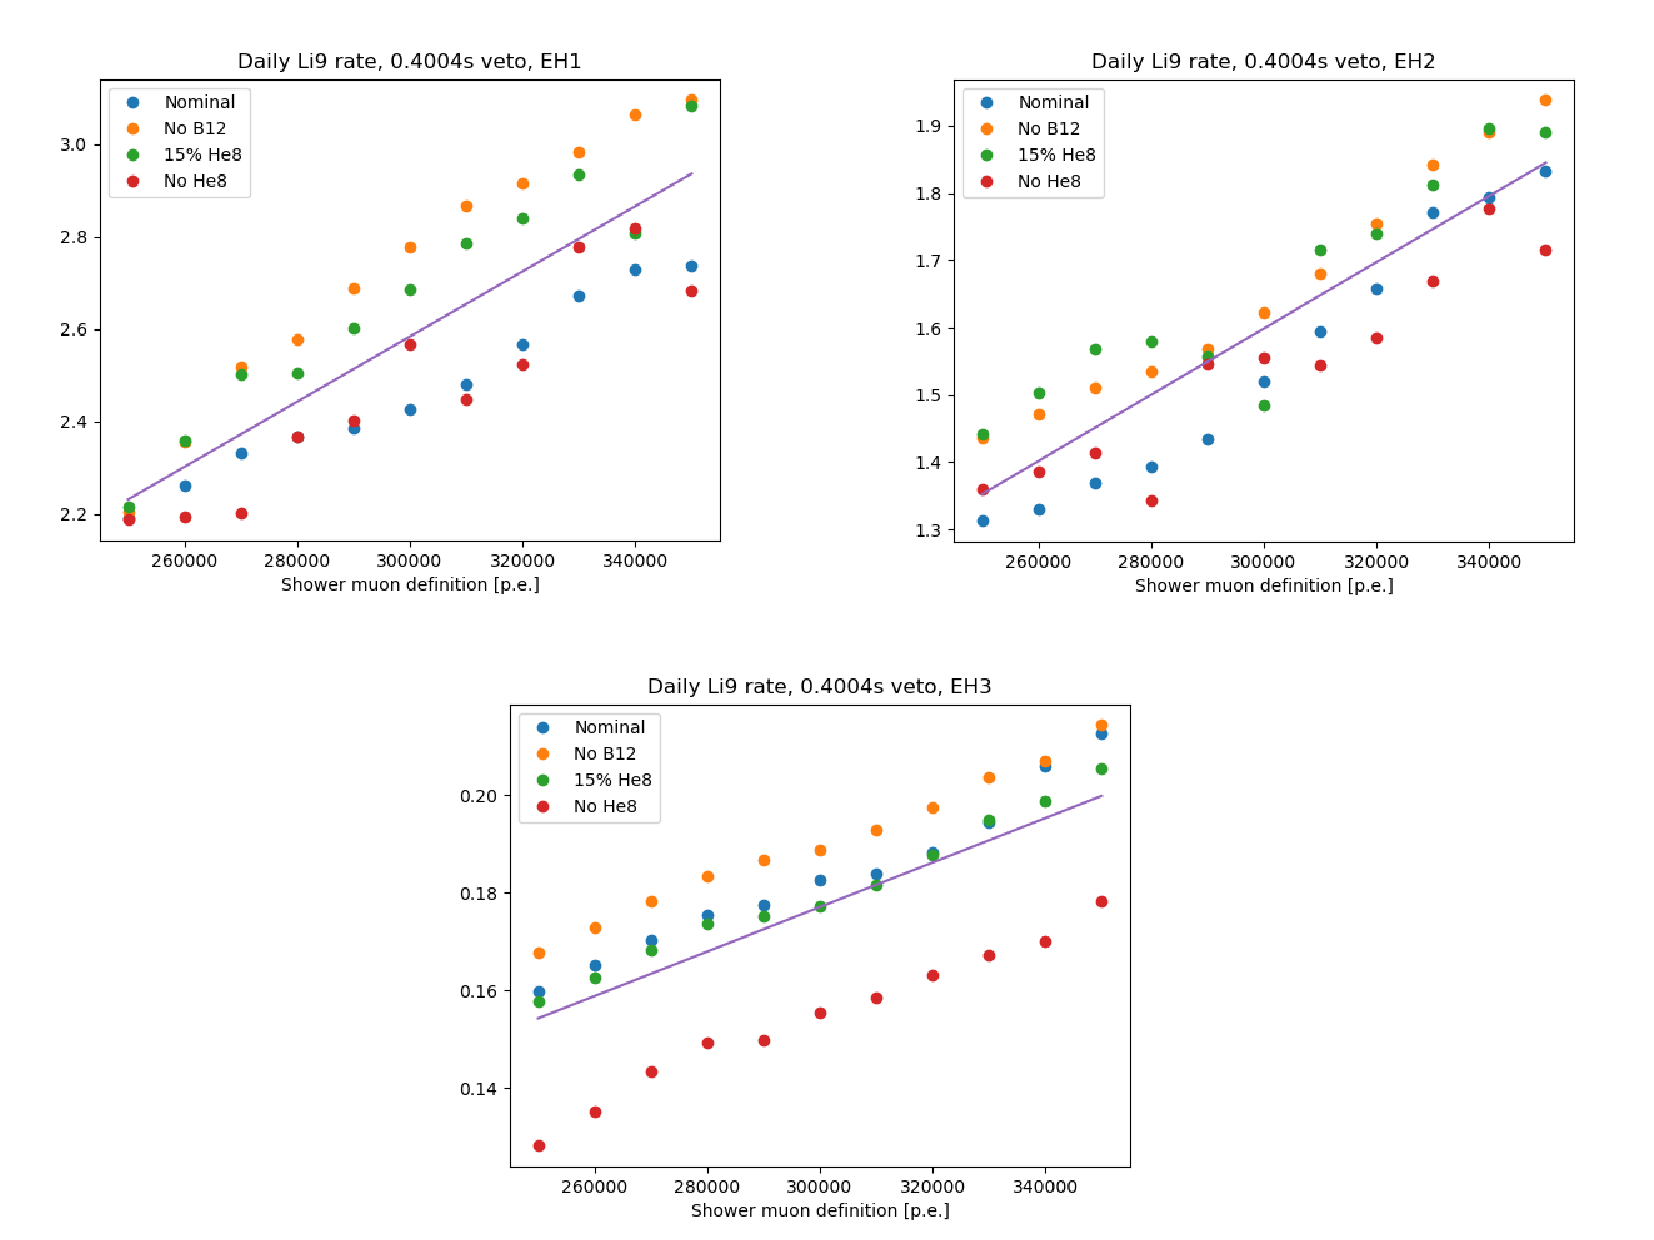
\includegraphics[scale=0.6]{Backgrounds/li9_linreg.pdf}
  \caption{Dependence of the measured $^9$Li rate (for the nominal shower-muon veto time of 0.4004~s) on the shower-muon threshold and the assumptions on the $^8$He fraction. The line-of-best-fit is used in determining the $^9$Li rate for arbitrary shower-muon tresholds in \autoref{chap:cutVary}.}
  \label{fig:bkgLi9Linreg}
\end{figure}

\begin{comment}
- forming and fitting the histogram %
- - Detail the cuts we use for different muon energy ranges (prompt energy, neutron tag)
- Prompt cut efficiency
- - Extraction of spectrum. Subtraction of IBD spectrum.
- - Uncertainty
- - - Statistical - binomial confidence interval accounting for error bars on subtracted spectrum => 1-2\% (See if can find how Chris did it in code... sounds tricky)
- - - Systematic - Variations in time binning, muon PE cut in background sample => 1\%
- Neutron tag efficiency
- - Uncertainty - 45\% according to doc-10920
- - Nominal value of... 80\%? 60\%?
- Uncertainty from fit
- - Neutron tagging cutoff - 1.5e5 to 1.8e5 => 10\% (NOT IN CHRIS'S TABLE)
- - Binning => <5\% (NOT IN CHRIS'S TABLE) (MENTIONED AT END)
- - B12 => 8\%
- - He8 => 4\%
- Uncertainty of shower veto correction (He8 fraction)
- - Vary He8 fraction from 0 to 15\%
- Conversion from fit result to daily rate
- - Efficiencies of Li9 selection (ntag, pcut)
- - IBD selection efficiencies (veto, mult)
- - Shower veto correction
- - Propagation of uncertainties
\end{comment}

\subsection{Spectrum}
\label{sec:bkgLi9Spectrum}

The \LiHe\ spectrum can be either extracted from data or predicted from nuclear tables. Both methods give consistent results (\autoref{fig:li9_spec}). The extracted spectrum (used for determining the efficiency of the prompt-energy cut in the $^9$Li selection) was described in \autoref{sec:bkgLi9PromptCutEff}. Largely for historical reasons, our background subtraction does not employ the extracted spectrum, instead using the predicted one. Here we briefly describe this prediction \cite{pedroLi9Spec1,pedroLi9Spec2}.

\begin{figure}[h]
  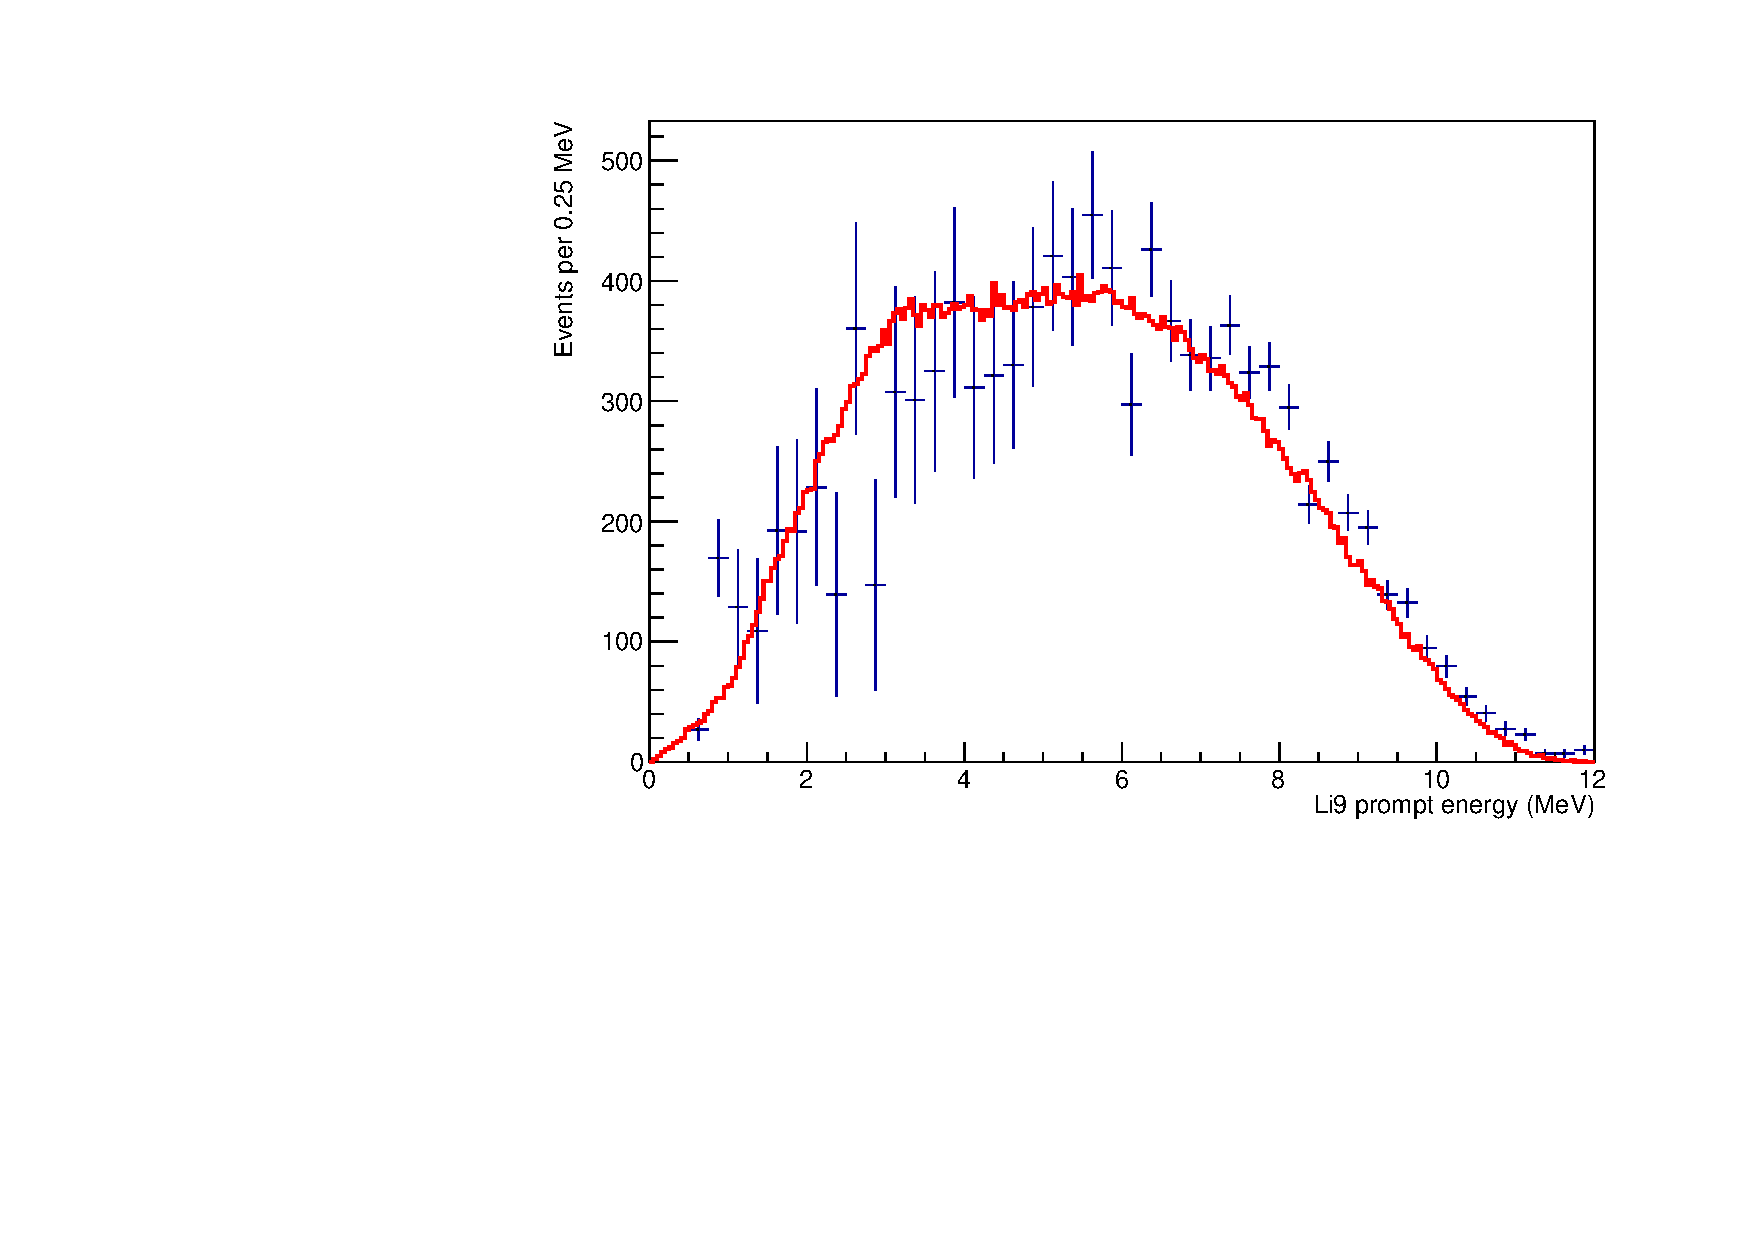
\includegraphics[width=0.5\textwidth]{Backgrounds/Li9/li9_spec_mine.pdf}
  \caption{Comparison of our extracted $^9$Li spectrum (blue points) with the predicted spectrum from \cite{pedroLi9Spec1,pedroLi9Spec2} (red line).}
  \label{fig:li9_spec}
\end{figure}

\begin{comment}
An extraction of the spectrum from Daya Bay data was performed by Marshall in [YYY]. The approach takes advantage of the fact that \LiHe\ are essentially the only IBD-like events that are correlated with muons on the 100~ms timescale. A \LiHe-enriched sample was obtained by taking IBD-like events within 2---200~ms of a ``shower'' muon, here defined as one producing at least $2\times10^5$ photoelectrons. This sample contained various muon-uncorrelated ``backgrounds'', such as true IBDs and accidentals. In order to remove this contamination, a \LiHe-depleted sample was obtained by looking for IBD candidates with no preceding shower muons within 1.5~s. Before subtracting the two spectra, an appropriate normalization for the depleted sample had to be determined. This was done by performing the time-to-last-muon fit for the enriched sample, which indicated the number of true \LiHe\ events in the sample, in turn implying the number of non-\LiHe\ events. The depleted sample was thus normalized to this latter count, and the subtraction was performed, giving the results shown in Fig.~YYY.
\end{comment}

For the prediction, three types of reference tables were consulted: nuclear structure, branching ratios, and measured spectra (of neutrons, alpha particles, and gamma-rays). Nuclear levels and decay schemes are shown in \Autoref{fig:li9_levels,fig:he8_levels}. Given the number of decay pathways involved, a purely analytic approach was infeasible (at least for $^9$Li), so a toy Monte Carlo was used to produce random decay events. The discussion here uses the example of $^9$Li, but $^8$He was essentially treated the same way. The initial $\beta$ decay (into any of four $^9\mathrm{Be}^*$ states) was simulated using the Fermi theory \cite{Fermi1934TentativoDU} and the published energy levels and branching fractions. For the decays that produce a $2\alpha+n$ final state (i.e. the only decays of interest to us), $^9\mathrm{Be}^*$ disintegrates via two consecutive two-body decays (via either $^8$Be or $^5$He). The angular distribution is assumed to be uniform. The disintegration was treated using basic kinematics, with the width of each state (\autoref{tab:bkgLi9Widths}) modeled with a Breit-Wigner function. The result was a collection of simulated events, each one recording the true energies of the electron, the neutron, and the two alphas (or, in the case of $^8$He, the electron, the neutron, and the gamma-ray).

\begin{figure}[h]
  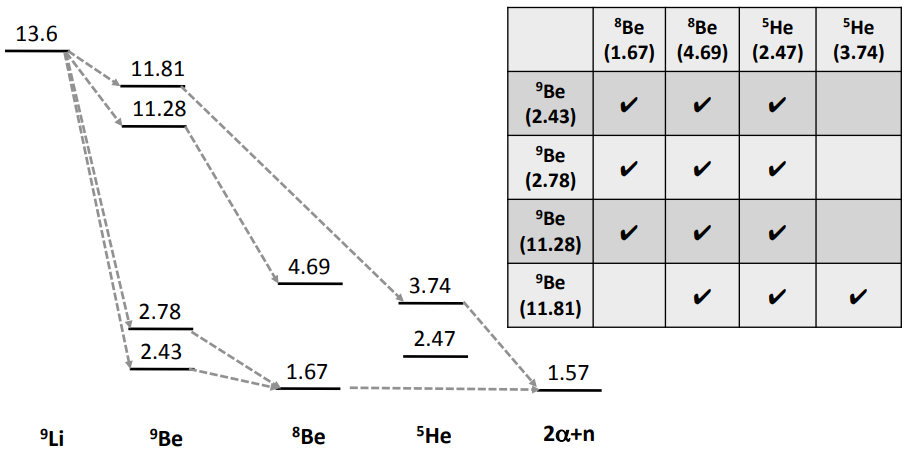
\includegraphics[scale=0.5]{Backgrounds/li9_levels.png}
  \caption{The decay of $^9$Li. Not all decays are shown with arrows. Energy levels are in MeV, relative to the ground state of $^9$Be. From \cite{pedroLi9Spec2}.}
  \label{fig:li9_levels}
\end{figure}

\begin{figure}[h]
  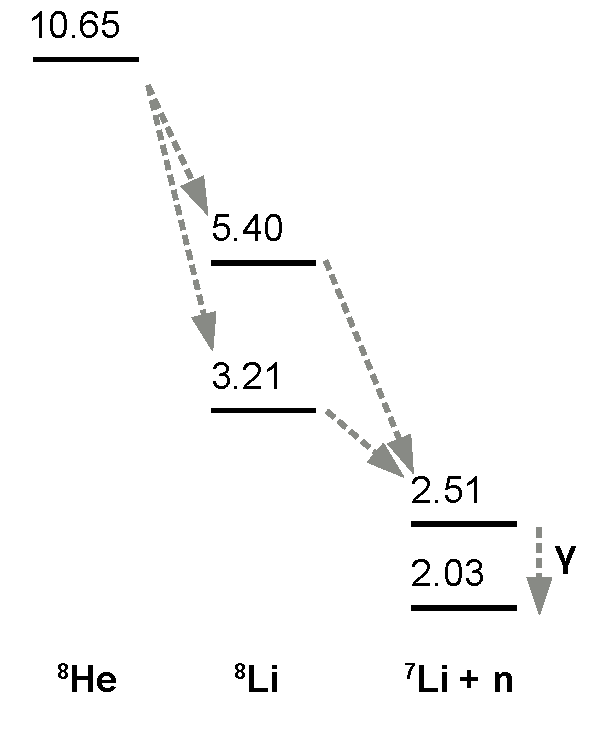
\includegraphics[scale=0.5]{Backgrounds/he8_levels.pdf}
  \caption{The decay of $^8$He. Energy levels are in MeV, relative to the ground state of $^8$Li.}
  \label{fig:he8_levels}
\end{figure}

\begin{table}[ht]
  \begin{tabular}{llcc}
    \toprule
    Parent & Daughter & Level (MeV) & Width (MeV) \\
    \midrule
    $^9$Li & $^9$Be & 11.81 & 0.400 \\
           & & 11.28 & 0.575 \\
           & & 2.78 & 0.110 \\
           & & 2.43 & $0.780 \times 10^{-3}$ \\
           & $^8$Be & 4.69 & $5.57 \times 10^{-6}$ \\
           & & 1.67 & 1.51 \\
           & $^5$He & 3.74 & 5.57 \\
           & & 1.67 & 0.648 \\
    \midrule
    $^8$He & $^8$Li & 5.40 & 0.650 \\
           & & 3.21 & 1.00 \\
           & $^7$Li & 2.51 & $9.02\times10^{-9}$ \\
           & & 2.03 & Stable \\
    \bottomrule
  \end{tabular}
  \caption{Widths of the nuclear excited states relevant for the prediction of the $^9$Li and $^8$He spectra \cite{ENDF}. For the daughters of $^9$Li ($^8$He), energy levels are expressed relative to the ground state of $^9$Be ($^8$Li).}
  \label{tab:bkgLi9Widths}
\end{table}

In order to benchmark this simulation, its output was compared against published measurements of \LiHe\ spectra of neutrons, alpha particles, and gamma-rays. Based on this comparison, one particularly broad level of $^8$He had to be augmented with a Gaussian density of states. Since the published branching ratios were relatively imprecise, they were hand-tuned (within limits) in the simulation so as to achieve satisfactory agreement with the published spectra.

Finally, to obtain the predicted spectrum in terms of prompt energy (i.e. reconstructed energy), the simulated events were passed through a model of the detector nonlinearity. Given that the \LiHe\ spectrum prediction was performed in 2013, it is based on an older nonlinearity model than the one discussed in \autoref{sec:fitToyDetResponse}.\footnote{The differences between models are not significant enough to warrant concern, especially in light of the uncertainty we assign to the \LiHe\ spectrum, as discussed in \cite{berkeley_toymc}.} Crucially, this model includes nonlinearity curves for the alpha particle and neutron, whose kinetic energies were also considered when determining the prompt energy for each event \cite{bcwNonlin}. The resulting prompt-energy spectra could then be combined according to the best estimate of the relative proportions of $^9$Li and $^8$He. For the sake of this analysis, a nominal 5.5\% fraction of $^8$He was used.\footnote{The measured spectrum and the rate fit both give results that are consistent with zero $^8$He, while rough predictions indicate that the $^8$He proportion should not exceed 20\%. (See the discussion of KamLAND on p.~\pageref{par:kamland_he8}.) Meanwhile, the predicted spectrum does not change very significantly when the fraction is varied from 0 to 15\%, in comparison to the other sources of uncertainty (neutron and alpha quenching). Hence, 5.5\%, an ``inherited'' feature of this analysis, is as good a guess as any.} \autoref{sec:fitToyBackgrounds} discusses the uncertainty assigned to the \LiHe\ spectrum.

\section{Cosmogenic fast neutrons}
\label{sec:bkgFastn}

As cosmic muons travel through the rock and other materials surrounding the ADs, they can eject energetic neutrons from the medium. If a fast neutron of the appropriate energy thermalizes and stops inside the AD, it will produce an IBD-like coincidence pair, in which the prompt signal consists largely of scintillation from the recoiled protons, and the delayed signal results from n-Gd capture. This process leads to a significant correlated background, amounting to some 20-30\% of that produced by cosmogenic isotopes. Two methods have been developed for estimating this background, the so-called \emph{extrapolation} and \emph{scaling} methods.

In the extrapolation method, the prompt-energy cut of the IBD selection is extended past 12 MeV to 100~MeV or beyond, where true IBDs are completely absent and the (largely flat) spectrum consists almost entirely of fast-neutrons events. This spectrum is then extrapolated below 12~MeV to estimate the fast-neutron component of the IBD sample, using a fit to a well-motivated model of the fast-neutron spectrum.

In the scaling method, a search is performed for the ``muon-tagged'' IBD-like events in the immediate aftermath of ``peripheral'' muons that only trigger the outer water pool. As with the extrapolation method, the prompt-energy cut is significantly extended. In the region above 12~MeV, where true IBDs are absent, a scaling factor can be determined from the ratio of muon-tagged to untagged events. Then, below 12~MeV, the tagged spectrum (which contains very few true IBDs due to the short post-muon time searched) is rescaled according to the scaling factor, yielding an estimate of the fast-neutron spectrum in the sub-12~MeV region.

The two methods are consistent to within 1--3\% (an order of magnitude smaller than the estimated uncertainty of each method), providing a high level of confidence in the estimation of the fast-neutron background. In the following sections, we describe these methods and their results, as obtained in \cite{fastn}.

\subsection{Event selection}
\label{sec:fastn_sel}

Two event samples are used in the fast-neutron analysis. The first, which we shall refer to as the ``untagged'' sample, is obtained using the standard IBD selection, as described in \autoref{chap:selection}, with the modification that the upper limit on the prompt energy is extended to 300~MeV instead of the usual 12~MeV. In this sample, the prompt spectrum below 12~MeV is essentially the same as the one used in the oscillation fit (i.e., dominated by true IBDs), whereas the high-energy region almost exclusively contains the (recoil protons from) fast-neutron events.

The other, ``tagged,'' sample contains IBD-like events that occur right after a muon that triggers \emph{only} the outer water pool. When a muon passes through the AD or the IWS, the resulting spallation products generate a significant amount of prompt activity in the AD. On the other hand, when a muon triggers only the OWS, without involvement of the IWS or AD, most of the debris is unable to penetrate into the GdLS. Fast neutrons, however, are an exception. The OWS tagging therefore provides a highly pure sample of fast neutrons for analysis.

The tagged sample is obtained by extending the upper cut to 300~MeV (as in the untagged sample) while disabling the standard muon veto. An additional requirement (see \autoref{fig:fastn_selection_diagram}) is that the prompt signal be timestamped within (-300, 600)~ns of an OWS trigger (defined by NHit $>$ 15, in this case). Furthermore, the delayed signal must occur at least 15 $\mu$s after the muon in order to eliminate Michel electrons, and there must be no AD or IWS muons within 600~\us\ of the OWS muon. This selection results in fairly low statistics (amounting to a few hundred events in the near halls), but the size of the sample is still sufficient to provide strong constraints on the fast-neutron background. This sample is statistically independent from the untagged sample, as all of its events would have been excluded by the (OWS) muon veto in the untagged selection.

\begin{figure}[h]
  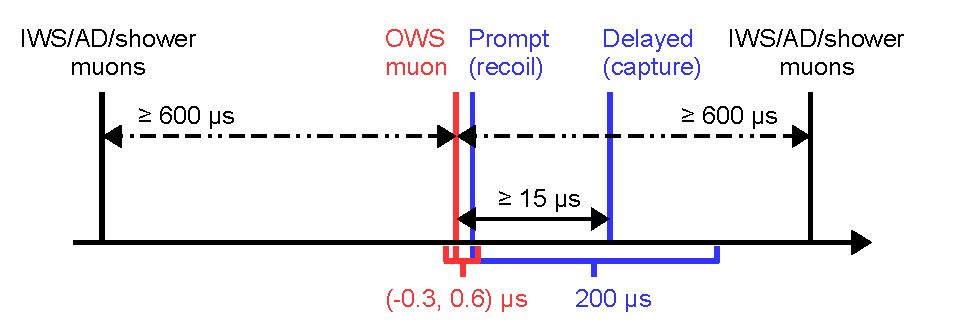
\includegraphics[width=0.9\textwidth]{Backgrounds/FastN/fastn_diagram_mine.pdf}
  \caption{Diagram illustrating the event selection scheme for the tagged fast-neutron sample.}
  \label{fig:fastn_selection_diagram}
\end{figure}

The prompt spectra from the two samples (scaled to have equal normalization above 12~MeV) are overlaid in \autoref{fig:fastn_prompt_energy_both_bz}, showing excellent agreement in the region between 12 and 150~MeV. Both samples are employed by the scaling method, as described next. Meanwhile, the extrapolation method only makes direct use of the tagged sample; however, the untagged sample still serves a role in validating the form of the fitting function used.

\begin{figure}[h]
  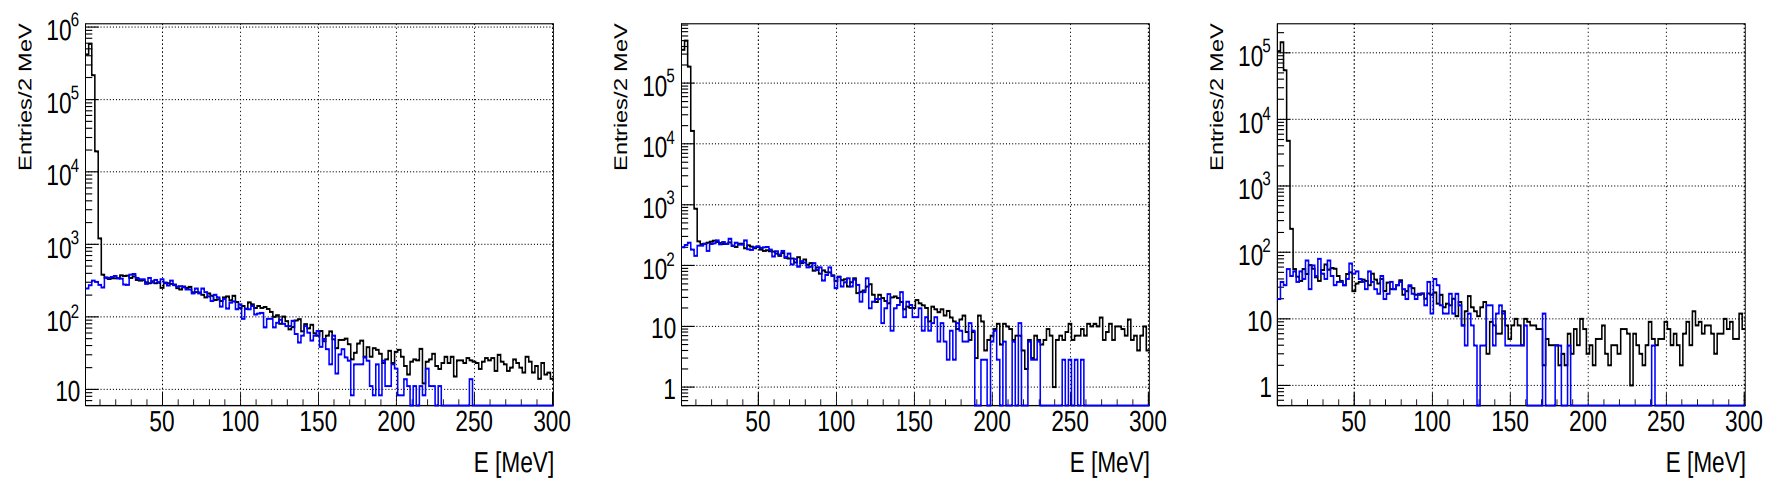
\includegraphics[width=\textwidth]{Backgrounds/FastN/prompt_energy_both_bz.png}
  \caption{Prompt spectra of the tagged (blue) and untagged (black) samples. The tagged spectrum has been rescaled to match the normalization of the untagged spectrum above 12~MeV. From \cite{fastn}.}
  \label{fig:fastn_prompt_energy_both_bz}
\end{figure}

\subsection{Scaling method}
\label{sec:fastn_scaling}

In the scaling method, we assume that the shape of the tagged spectrum is an accurate representation of the shape of the fast-neutron background. In other words, we assume that, for any given fast neutron, there is no energy dependence on the probability of its association with an OWS-only muon. Previous studies within the collaboration have supported the validity of this assumption.

\def\emax{\ensuremath{E_\mathrm{max}}} \def\ntag{\ensuremath{N_\mathrm{tag}}}
\def\nuntag{\ensuremath{N_\mathrm{untag}}}

We define the \emph{scaling factor} $F$ as
\begin{equation}
  F(\emax) = \frac{\nuntag[12, \emax]}{\ntag[12, \emax]},
\end{equation}
i.e., the ratio of the integral of the two samples between 12~MeV and \emax. The dependence on \emax\ reflects the arbitrary choice of the upper energy limit, which contributes to the uncertainty on the result (primarily due to stastical fluctuations in the small sample of tagged neutrons). This uncertainty is quantified by comparing the results for \emax\ of 80, 100, 120, and 150~MeV (\autoref{fig:fastn_scaling_factor}) \cite{fastn} , resulting in an estimated systematic uncertainty given by the half-range divided by the mean, as listed in \autoref{tab:bkgFastnUnc}. In addition, for a \emph{fixed} \emax, there is a purely statistical uncertainty\footnote{As noted previously, the tagged and untagged samples are statisically independent.},
\begin{equation}
  \sigma_F(\emax) = F \cdot \sqrt{\nuntag^{-1}[12, \emax] + \ntag^{-1}[12,
      \emax]},
\end{equation}
which also contributes to the final uncertainty.

\begin{figure}[h]
  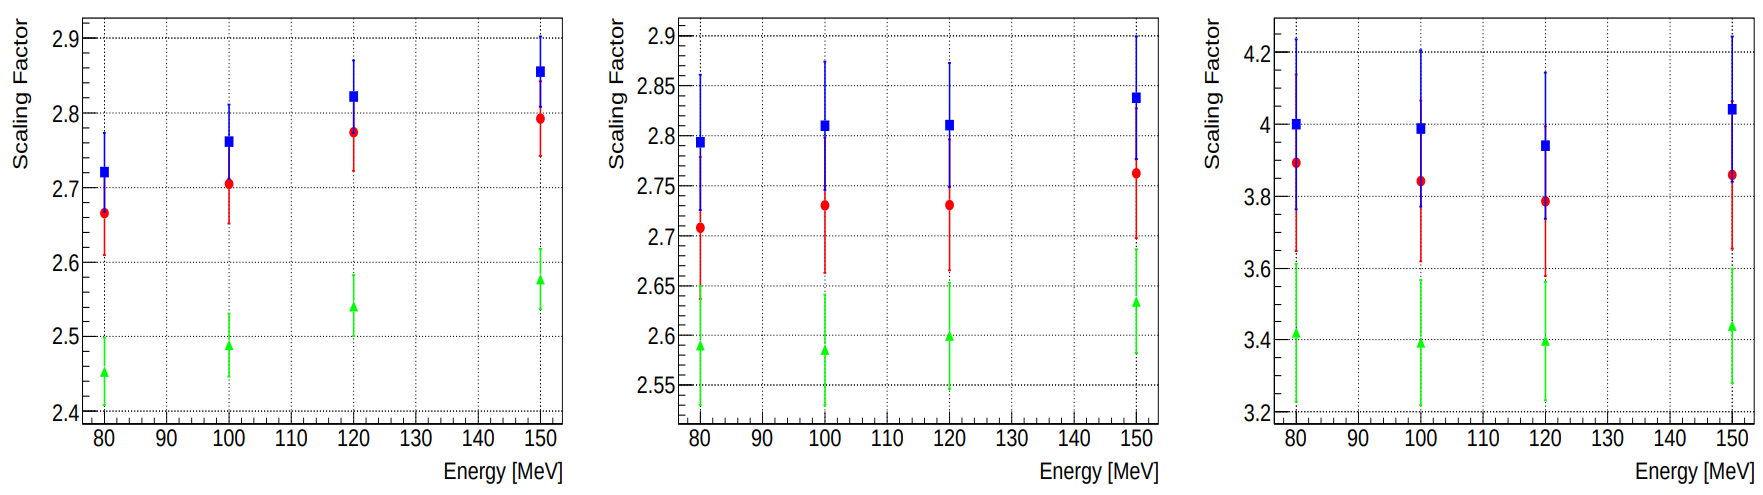
\includegraphics[width=\textwidth]{Backgrounds/FastN/scaling_factor.png}
  \caption{Comparison of the scaling factor $F(E_{\mathrm{max}})$ obtained for different values of $E_{\mathrm{max}}$. The three colors correspond to different IBD selection criteria, with the blue squares representing the criteria used in this analysis. From \cite{fastn}.}
  \label{fig:fastn_scaling_factor}
\end{figure}

\def\nfn{\ensuremath{N_\mathrm{FN}}} \def\rfn{\ensuremath{R_\mathrm{FN}}}

For the standard IBD selection, the number of fast neutrons within the fiducial energy range of [0.7, 12]~MeV is determined simply as
\begin{equation}
  \nfn = F \cdot \ntag[0.7, 12].
\end{equation}
Its statistical uncertainty, in turn, is
\begin{equation}
  \label{eq:fastn_scal_unc}
  \sigma_\mathrm{FN} = \sqrt{\ntag^2[0.7, 12]
    \cdot \sigma_F^2 + F^2 \cdot \ntag[0.7, 12]}.
\end{equation}
Finally, the normalized daily fast-neutron rate is
\begin{equation}
  \label{eq:fastn_rate}
  \rfn = \frac{\nfn}{T_\mathrm{DAQ} \cdot \epsilon_\mu \cdot \epsilon_m},
\end{equation}
where $T_\mathrm{DAQ}$, $\epsilon_\mu$, and $\epsilon_m$ are the DAQ livetime, muon veto efficiency, and multiplicy cut efficiency for the untagged sample. The resulting $\rfn$, for the four different values of $E_{\mathrm{max}}$, are plotted in \autoref{fig:fastn_rate_vs_scaling}.

% This value is then combined with the extrapolation result, described next, and a total uncertainty is assigned to the combination.

\begin{figure}[h]
  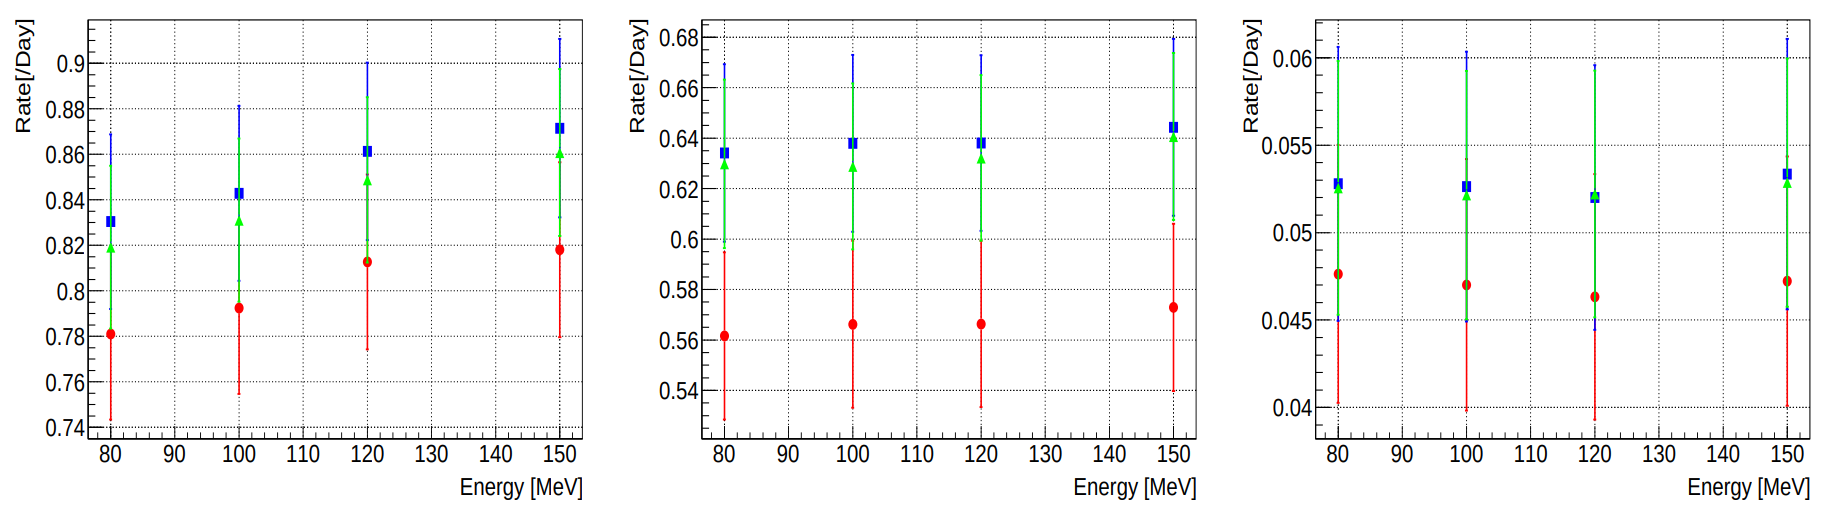
\includegraphics[width=\textwidth]{Backgrounds/FastN/rate_vs_scaling.png}
  \caption{Daily fast-neutron rate from the scaling method, as a function of $E_{\mathrm{max}}$. The blue squares correspond to the IBD selection criteria used in this analysis. From \cite{fastn}.}
  \label{fig:fastn_rate_vs_scaling}
\end{figure}

\subsection{Extrapolation method}
\label{sec:fastn_extrap}

Previous simulation studies have found that the fast neutron spectrum can be accurately described by the PDF
\begin{equation}
  \label{eq:bkgFastnShape}
  f(E; E_0, a) = A \cdot \left( \frac{E}{E_0} \right)^{-a-E/E_0},  
\end{equation}
where $E_0$ and $a$ are shape parameters, and $A(E_0, a)$ normalizes the PDF. When a measured fast-neutron spectrum is then fit to the form
\begin{equation}
  \label{eq:bkgFastnScaledPDF}
  S(E; N, E_0, a) = N \cdot f(E; E_0, a),
\end{equation}
the best-fit value of $N$ represents the number of events ``under the curve'' from 0 to $\infty$~MeV.

In turn, if we have a (hypothetical) pure fast-neutron spectrum containing $\nfn$ events in the fiducial region of [0.7, 12]~MeV, then the full spectrum ([0, $\infty$]~MeV) should contain an event count equal to
\begin{equation}
  N = \frac{\nfn}{\int_{0.7}^{12} f(E; E_0, a)\,dE }.
\end{equation}
Here, the denominator represents the fiducial region's fraction of the total spectrum. Substituting this form of $N$ into \autoref{eq:bkgFastnScaledPDF}, and allowing the floated parameter to be $\nfn$ instead of $N$, we obtain the form
\begin{equation}
  \label{eq:fastn_extrap_form}
  S(E; \nfn, E_0, a) = \frac{\nfn}%
  {\int_{0.7}^{12} E'^{-a-E'/E_0} \, dE'} E^{-a-E/E_0}.
\end{equation}
When \autoref{eq:fastn_extrap_form} is then fit to the measured fast-neutron spectrum, the best-fit $\nfn$ indicates the number of events in the fiducial region. The key to the extrapolation method is that this fit is performed outside the fidicial region, where the fast-neutron sample is uncontaminated.

The validity and robustness of \autoref{eq:fastn_extrap_form} was verified by fitting it to the OWS-tagged samples from each hall (\autoref{fig:fastn_ows_fit_bz}) \cite{fastn}. Four fitting ranges were used, all starting at 0.7~MeV, and ending at 80, 100, 120, and 150~MeV. All fits produced satisfactory goodness-of-fit and consistent values of $E_0$ (\autoref{fig:fastn_par_E0_ows}). Disabling of the $a$ parameter was found to introduce negligible differences.

\begin{figure}[ht]
  \begin{minipage}{0.333\textwidth}%
    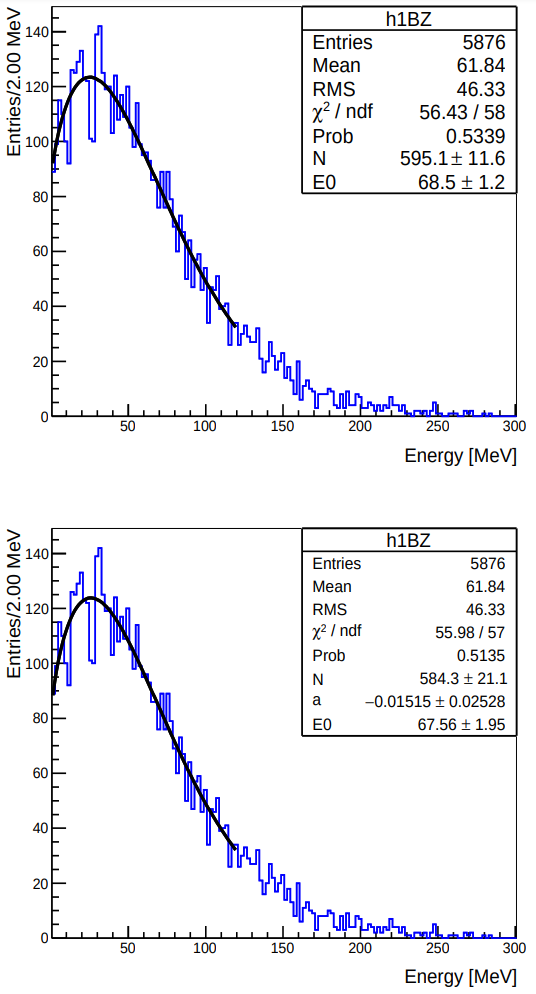
\includegraphics[width=\textwidth]{Backgrounds/FastN/ows_fit_eh1_bz.png}%
  \end{minipage}%
  \begin{minipage}{0.333\textwidth}%
    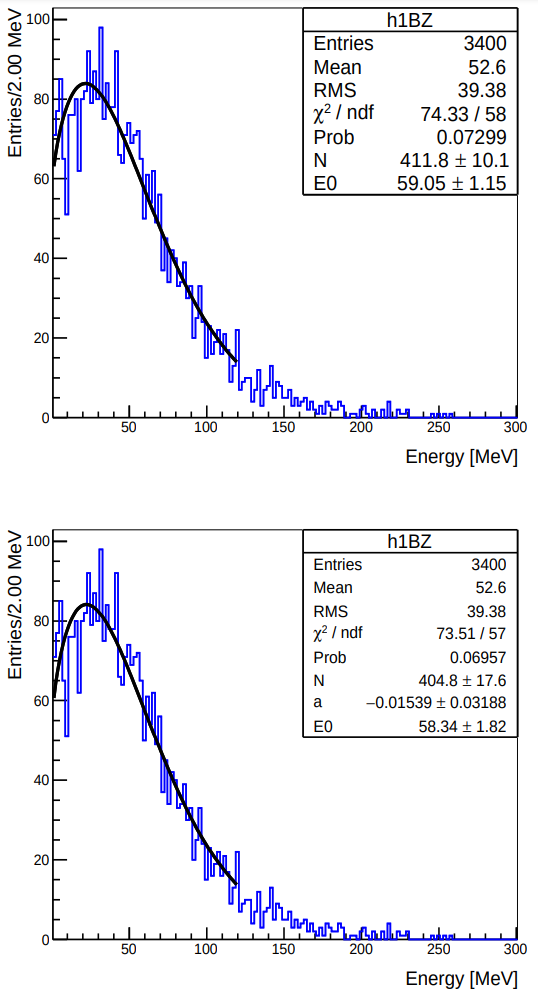
\includegraphics[width=\textwidth]{Backgrounds/FastN/ows_fit_eh2_bz.png}%
  \end{minipage}%
  \begin{minipage}{0.333\textwidth}%
    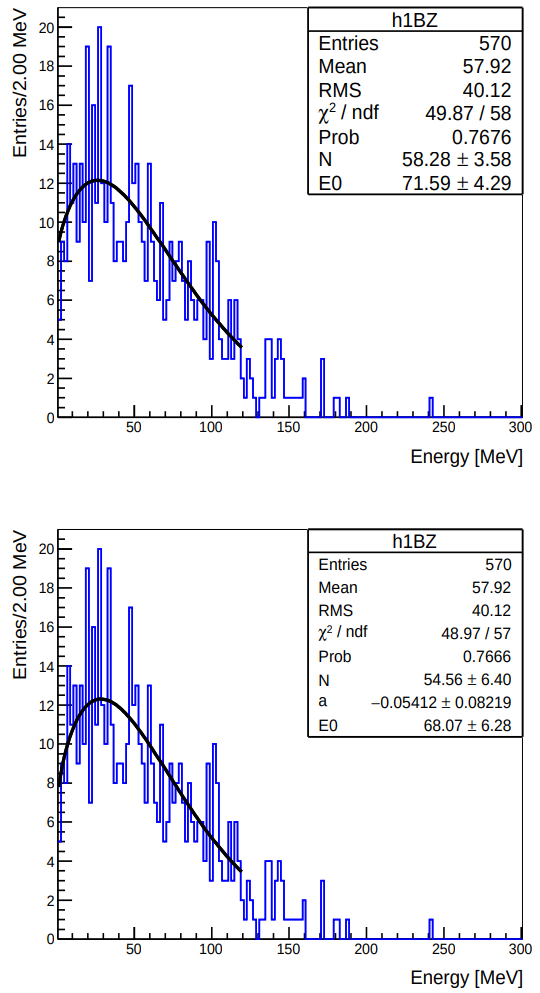
\includegraphics[width=\textwidth]{Backgrounds/FastN/ows_fit_eh3_bz.png}%
  \end{minipage}%
  \caption{Fits of the OWS-tagged fast-neutron spectra to \autoref{eq:fastn_extrap_form} for EH1 (left), EH2 (center), and EH3 (right). From \cite{fastn}.}
  \label{fig:fastn_ows_fit_bz}
\end{figure}

\begin{figure}[ht]
  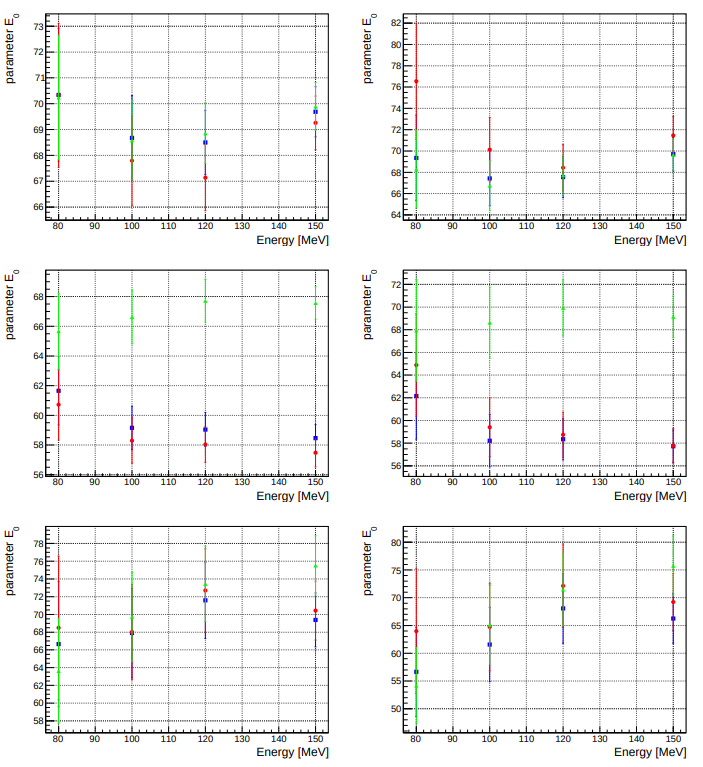
\includegraphics[scale=0.5]{Backgrounds/FastN/par_E0_ows.png}
  \caption{Values of $E_0$ obtained from fitting the OWS-tagged fast-neutron samples to \autoref{eq:fastn_extrap_form}. The parameter $a$ was fixed to zero for the plots on the left, while it was allowed to float for the plots on the right. The blue squares correspond to the IBD selection criteria used in this analysis. From \cite{fastn}}
  \label{fig:fastn_par_E0_ows}
\end{figure}

Finally, the fit was performed on the untagged sample (\autoref{fig:fastn_ibd_fit_bz}), using the same four upper limits as before, but with the lower limit set to 12~MeV.  As with the scaling method, each value of $\nfn$ was converted to a livetime- and efficiency-normalized daily rate according to \autoref{eq:fastn_rate} (\autoref{fig:fastn_rate_vs_fit_range}). The spread between the resulting four values was incorporated into the total uncertainty, as described in the next section.

\begin{figure}[ht]
  \begin{minipage}{0.333\textwidth}%
    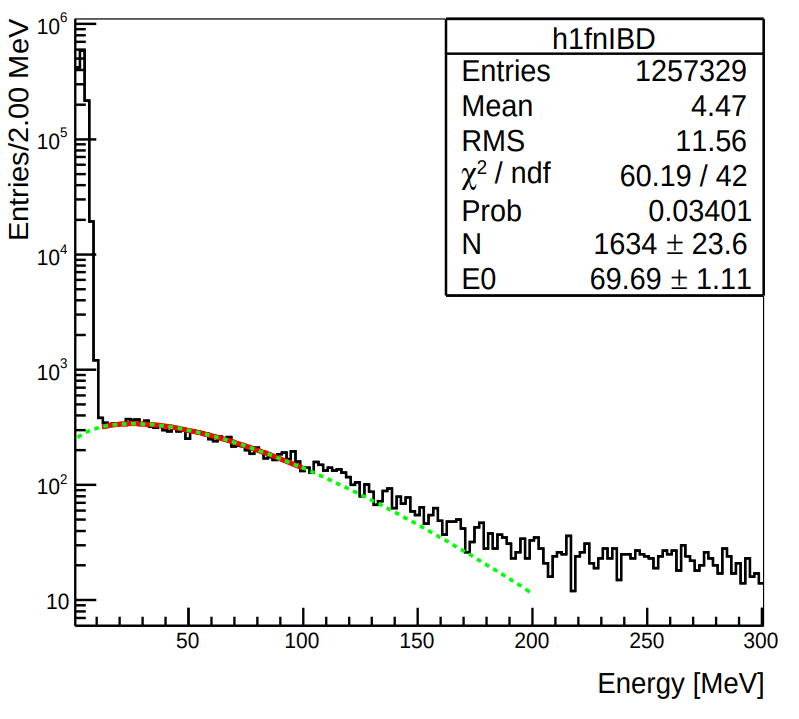
\includegraphics[width=\textwidth]{Backgrounds/FastN/ibd_fit_eh1_bz.png}%
  \end{minipage}%
  \begin{minipage}{0.333\textwidth}%
    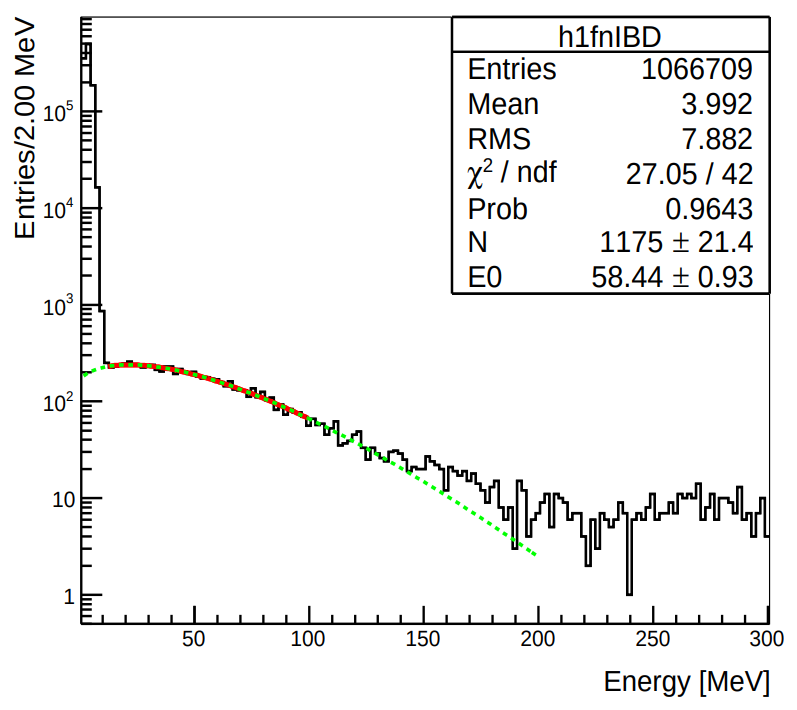
\includegraphics[width=\textwidth]{Backgrounds/FastN/ibd_fit_eh2_bz.png}%
  \end{minipage}%
  \begin{minipage}{0.333\textwidth}%
    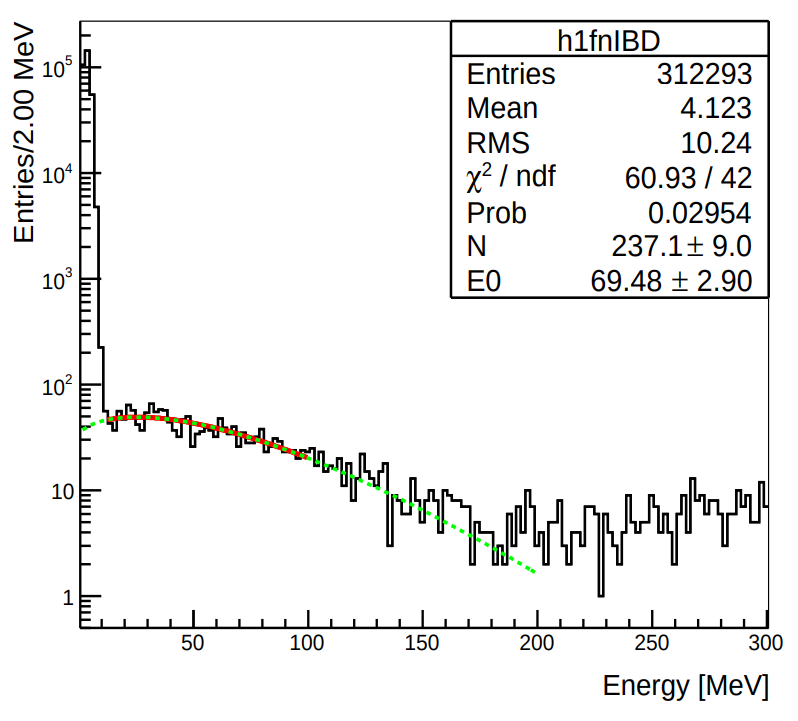
\includegraphics[width=\textwidth]{Backgrounds/FastN/ibd_fit_eh3_bz.png}%
  \end{minipage}%
  \caption{Fits of the untagged fast-neutron spectra to \autoref{eq:fastn_extrap_form} for EH1 (left), EH2 (center), and EH3 (right). From \cite{fastn}.}
  \label{fig:fastn_ibd_fit_bz}
\end{figure}

\begin{figure}[h]
  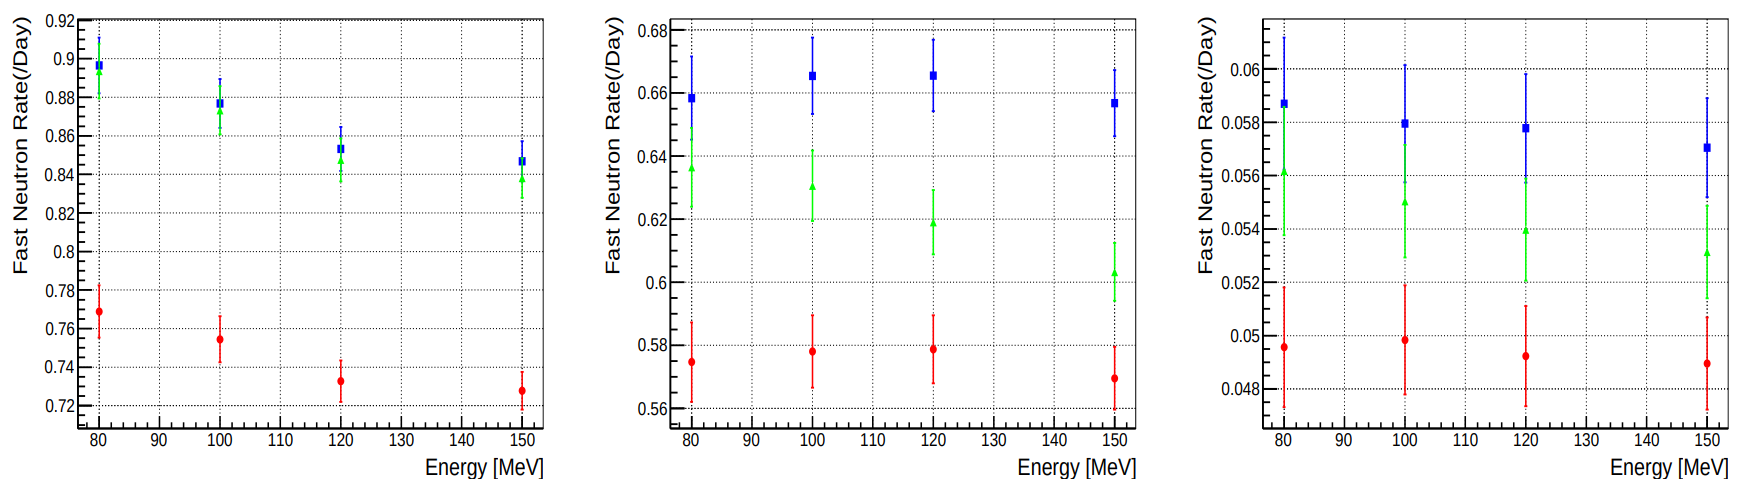
\includegraphics[width=\textwidth]{Backgrounds/FastN/rate_vs_fit_range.png}
  \caption{Daily fast-neutron rates from the extrapolation method, as a function of the upper limit of the fit range. The blue squares correspond to the IBD selection criteria used in this analysis. From \cite{fastn}.}
  \label{fig:fastn_rate_vs_fit_range}
\end{figure}

\subsection{Final result and total uncertainty}
\label{sec:fastn_comb}

In total, eight consistent estimates of \rfn\ were obtained for each hall, derived from four scaling ranges in the scaling method, and four fitting ranges in the extrapolation method \cite{fastn}. As in the official Daya Bay analysis, we arbitrarily choose the 12-100~MeV scaling method as the source of the daily fast neutron rates in this analysis.

Six uncertainties were added in quadrature to obtain the total \cite{fastn}:
\begin{itemize}
\item Statistical: The statistical uncertainty on the scaling factor $F$, described by \autoref{eq:fastn_scal_unc}.
\item Scaling range: The uncertainty from the choice of scaling range, which was determined from the difference between the highest and lowest fast-neutron rates across the four ranges used.
\item Fit range: The analogue for the choice of the fitting range.
\item Fit result: The statistical uncertainty in the fitted value of $N_\mathrm{fid}$.
\item Bin width: From the dependence of the fit results on the choice of binning, which was determined by varying the bin widths and repeating the fits.
\item Methods: From the difference in results between the scaling and extrapolation methods.
\end{itemize}
These uncertainties are summarized in \autoref{tab:bkgFastnUnc}, and the final results given in \autoref{tab:bkgFastnFinalRates}.

\begin{table}[ht]
  \begin{tabular}{lccc}
    \toprule
    Uncertainty (\%)            & EH1  & EH2  & EH3 \\
    \midrule
    Statistical & 4.6 & 5.5 & 14.7 \\
    Scaling range & 2.4 & 0.8 & 1.2 \\
    Fit range & 2.9 & 0.6 & 0.8 \\
    Fit result & 1.5 & 1.8 & 4.0 \\
    Bin width & 0.4 & 0.4 & 2.0 \\
    Methods & 7.7 & 7.7 & 7.7 \\
    \midrule
    Total & 9.8 & 9.7 & 17.2 \\
    \bottomrule
  \end{tabular}
  \caption{Uncertainty budget for the fast-neutron rates \cite{fastn}.}
  \label{tab:bkgFastnUnc}
\end{table}

\begin{table}[ht]
  \begin{tabular}{lccc}
    \toprule
    EH1 & EH2 & EH3 \\
    \midrule
    0.843 $\pm$ 0.083 & 0.638 $\pm$ 0.062 & 0.053 $\pm$ 0.009 \\
    \bottomrule
  \end{tabular}
  \caption{Final estimated fast-neutron rates (per AD per day) \cite{fastn}.}
  \label{tab:bkgFastnFinalRates}
\end{table}

\newcommand\AmC{$^{241}$Am-$^{13}$C}

\section{AmC source}
\label{sec:bkgAmC}

To study the response of the detectors to neutrons, each AD was initially configured with a low-intensity ($\sim$0.7~Hz) \AmC\ neutron source in each of the three automated calibration units (ACUs) housed on the detector's lid. The \AmC\ sources are used, for instance, in determining the ratio of visible energies between $^{60}$Co and n-Gd events; this ratio is a necessary input in the calibration of the AdScaled reconstruction. In contrast to more traditional neutron sources such as $^{252}$Cf and $^{241}$Am-$^{9}$Be, the \AmC\ source was designed to avoid multi-neutron and gamma-neutron cascades (a potential correlated background). Furthermore, when not in use, the location and shielding of the sources ensures that neutrons do not infiltrate the GdLS region, protecting against correlated backgrounds from proton recoils followed by neutron capture.

In spite of these precautions, a rare mechanism can still produce correlated backgrounds: A neutron may scatter inelastically in the stainless steel against Fe, Cr, Mn, or Ni, producing prompt gamma rays (generally totalling less than 3~MeV of reconstructed energy), before thermalizing and being captured either by one of these four elements or by Gd in the GdLS overflow tank (producing a signal between 6 and 12~MeV). Although many of these gamma rays do not reach the scintillator, some do, and when this happens for both the prompt and delayed gamma rays, the resulting pair can sometimes pass the IBD selection criteria.

The first experimental suggestion of this background came from an observed excess of neutron-like (i.e. 6--12 MeV) \emph{uncorrelated} events in the top half of the detector (\autoref{fig:amc_z_dist}). The expected neutron-like events (primarily fast neutrons and decays of cosmogenic $^{12}$B) are predicted to display vertical symmetry (as was explicitly confirmed for a high-purity sample of $^{12}$B candidates), so the asymmetric nature of this excess implicated the \AmC\ source as the origin. Subsequent MC simulations showed that these uncorrelated events (from neutron capture in the SS or Gd overflow tank) are associated with a correlated background. The evaluation of this so-called AmC background is detailed in \cite{Gu_2016}; here we briefly summarize the procedure and its results.

\begin{figure}[ht]
  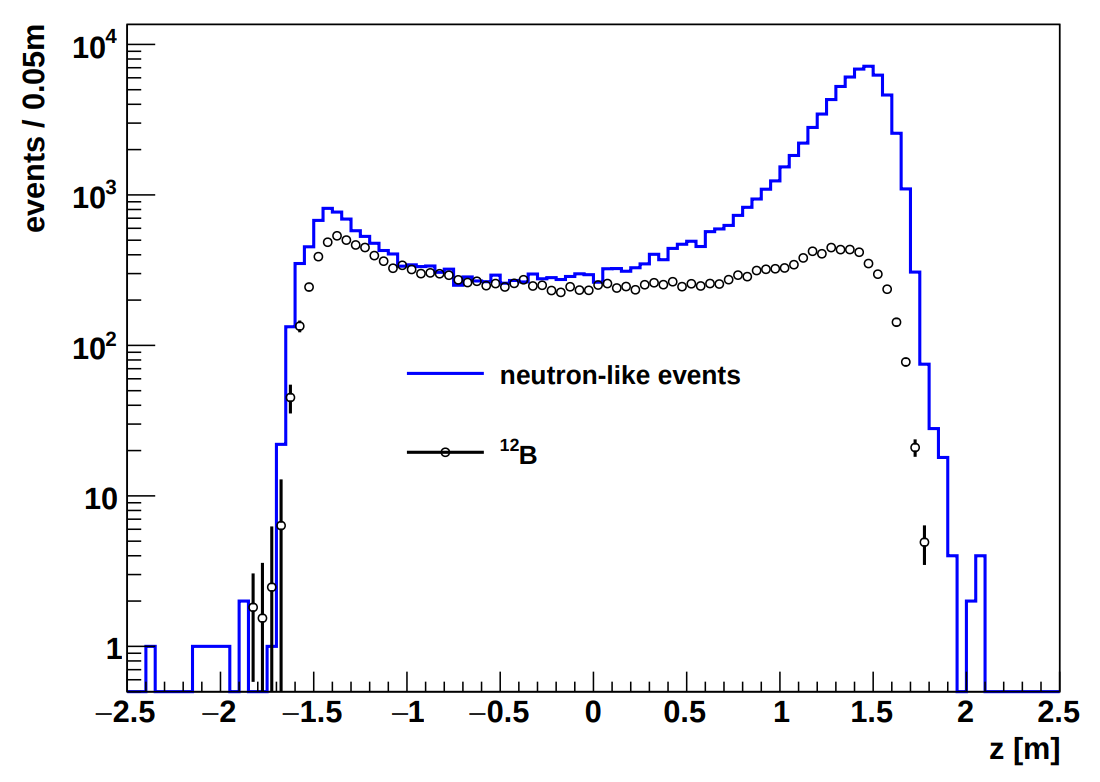
\includegraphics[scale=0.4]{Backgrounds/AmC/z_dist.png}
  \caption{Vertical distribution of uncorrelated neutron-like events, illustrating an excess in the upper half of the AD due to the AmC source in the ACUs \cite{Gu_2016}.}
  \label{fig:amc_z_dist}
\end{figure}

At first glance, the AmC background could be measured simply by removing the AmC sources from one detector and comparing the IBD candidate rate to an adjacent detector. However, given the low rate of this process (0.2--0.3 events/day/AD when all three AmC sources are installed) and the substantial ``background'' from IBDs, it would take an impractical amount of time to accumulate sufficient statistics, and the AdScaled calibration would be impaired in the meantime. On the other hand, it \emph{is} possible to directly measure the rate ($\sim$230/day, initially) of \emph{uncorrelated} events from neutron capture in the stainless steel. Furthermore, MC simulations can be used to relate the rates of uncorrelated and correlated events. Finally, a high-activity AmC source (HAS) can be used to benchmark the MC. These three insights together enable a relatively good (i.e. to within 45\%) determination of the AmC background.

The following is the fundamental relationship used in the AmC background estimation:
\begin{equation}
  \label{eq:bkgAmcFundamental}
  R_{\mathrm{corr}} = R_{\mathrm{uncorr}} \times \xi = R_{\mathrm{uncorr}} \times \int_{0.7}^{\SI{12}{MeV}} f(E)\,dE.
\end{equation}
Here, $R_{\mathrm{uncorr}}$ is the rate of uncorrelated neutron-like events produced by the AmC source, as measured directly from ordinary data. Meanwhile, $\xi$ is the ratio of correlated to uncorrelated events, as determined from a combination of simulations and HAS data. The factor $f(E)$ is simply the differential value of $\xi$ as a function of prompt energy; i.e. $f(E)\,dE$ is the number of correlated events with a prompt energy in [$E$, $E + dE$], per uncorrelated neutron-like event.

$R_{\mathrm{uncorr}}$ was measured trivially, simply by taking the difference in the number of neutron-like events between the top and bottom halves of each AD. All of the complexity lay in the determination of $\xi$. In principle, $\xi$ could be extracted directly from a MC simulation. Although the Daya Bay MC contains a detailed and accurate modeling of the detector materials and geometry (including the ACUs and the AmC sources themselves), any inaccuracies in the simulated physics could bias the obtained value of $\xi$. Accordingly, the HAS was designed and deployed in order to validate the simulations.

Compared to the AmC calibration source, with a rate of $\sim$0.7~Hz, the HAS was much more intense, producing $\sim$59 neutrons/s. Furthermore, the enclosure of the HAS consisted of a nearly solid cylinder of stainless steel, in order to maximize the rate of neutron captures and inelastic scatters. The HAS was placed on the lid of EH3-AD1 (named AD4) in the summer of 2012, and data was collected for ten days. The number of uncorrelated HAS-induced neutron-like events was determined by subtracting the neutron-like samples between AD4 and the adjacent AD5, which observed $\sim$50,000 and $\sim$4,000 events, respectively (\autoref{fig:amc_single_spec_2ad})

\begin{figure}[ht]
  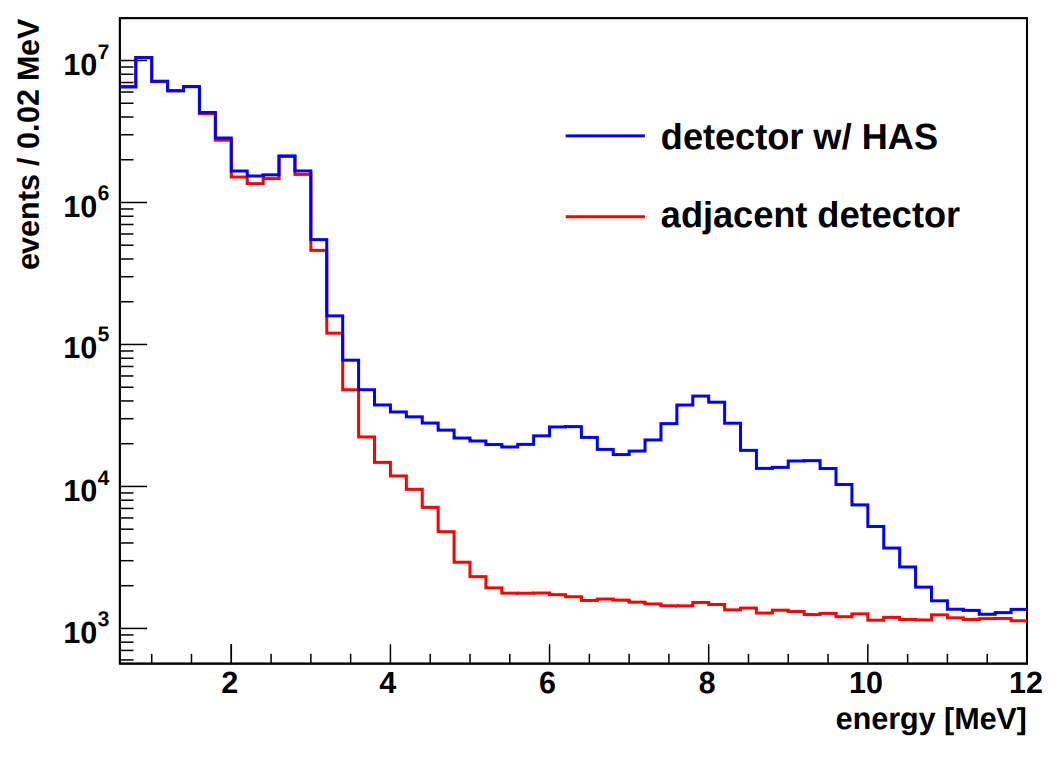
\includegraphics[scale=0.4]{Backgrounds/AmC/single_spec_2ad.png}
  \caption{Spectra of uncorrelated events (singles) in the HAS-deployed AD and an adjacent AD, showing a clear excess of neutron-like events from the HAS \cite{Gu_2016}.}
  \label{fig:amc_single_spec_2ad}
\end{figure}

Meanwhile, the number of \emph{correlated} AmC events was measured by taking the spectrum of IBD candidates in AD4, subtracting the accidental background, and then subtracting the (background-subtracted) IBD sample measured by AD5 (\autoref{fig:amc_prompt_spec_data}).\footnote{This procedure doesn't account for other correlated backgrounds in AD4, such as $^9$Li and fast neutrons, but their rates of $< 0.2$/d are insignificant compared to the 63 correlated events per day produced by the HAS.} The delayed spectrum from this sample, consisting of the sum of neutron capture peaks from Fe, Ni, Cr, and Mn, demonstrated excellent agreement with the prediction of the MC, proviing further validation of the MC's predictions (\autoref{fig:amc_ncap_spec_mc}). Relating the uncorrelated and correlated rates gave a value of $\xi$, \emph{for the HAS}, of $(1.5\pm0.3)\times10^{-3}$. The Geant4 MC, on the other hand, returned a $\xi$ of $(1.2\pm0.1)\times10^{-3}$ for the HAS. The 25\% difference versus data was then assigned as the uncertainty (and bias) of the MC. With the addition in quadrature of the 20\% statistical uncertainty in the data, a total uncertainty of 30\% was assigned to $\xi$.

\begin{figure}[ht]
  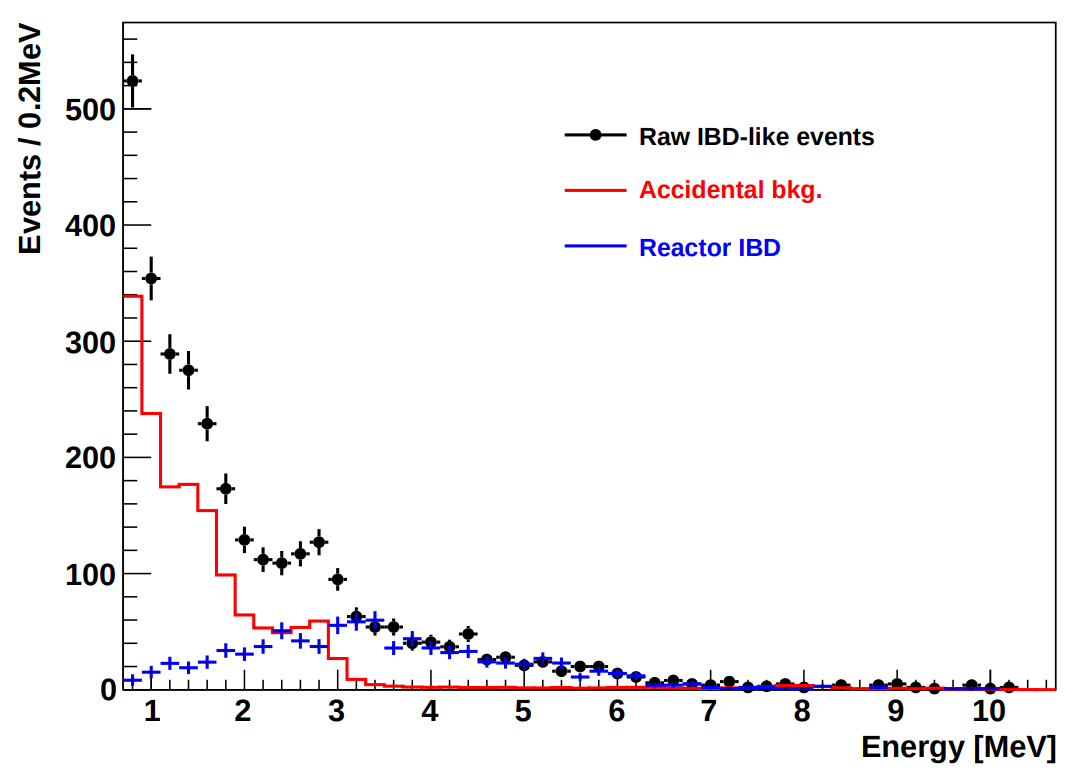
\includegraphics[scale=0.4]{Backgrounds/AmC/prompt_spec_data.png}
  \caption{Prompt spectrum of IBD-like events in the HAS-deployed detector, along with the spectrum of accidentals (determined from the singles spectrum) and the (background-subtracted) reactor IBD spectrum from an adjacent AD. From \cite{Gu_2016}.}
  \label{fig:amc_prompt_spec_data}
\end{figure}

\begin{figure}[ht]
  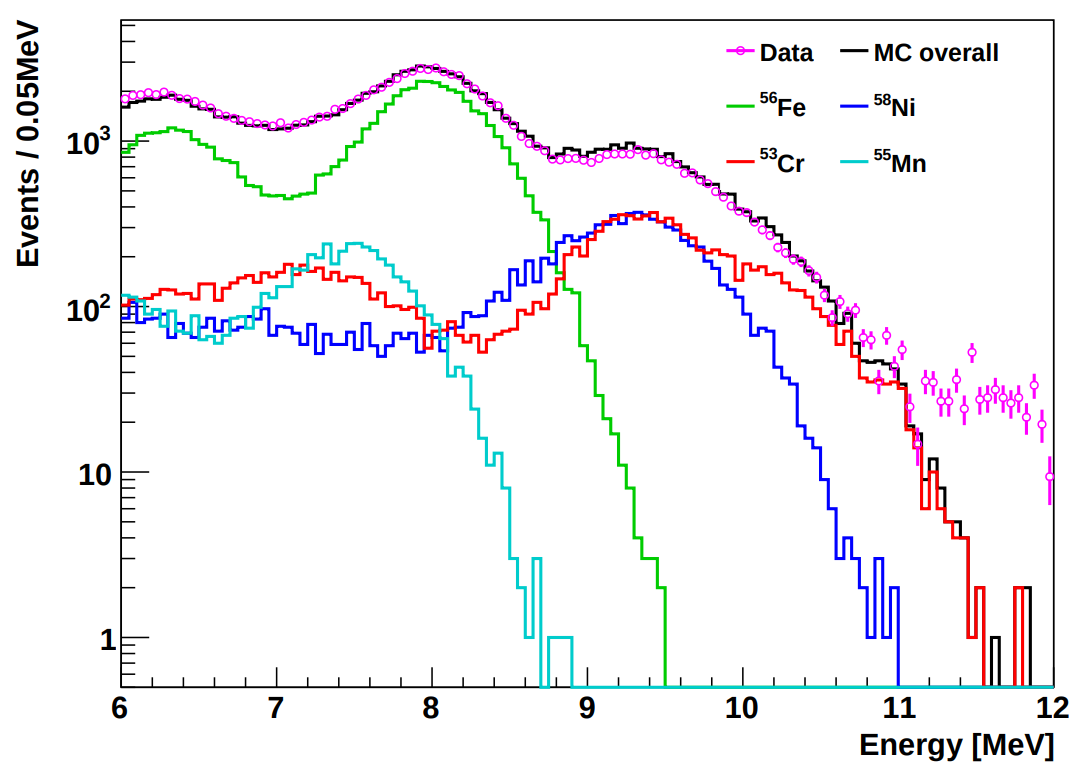
\includegraphics[scale=0.4]{Backgrounds/AmC/ncap_spec_mc.png}
  \caption{Comparison of the AmC delayed spectrum between data and the MC, showing the latter's contributions from the individual neutron capture peaks. From \cite{Gu_2016}.}
  \label{fig:amc_ncap_spec_mc}
\end{figure}

Compared to the HAS, the ordinary, i.e. low-intensity, AmC source (LAS) is expected to have a lower $\xi$, since it lies farther from the AD and has a lower density of surrounding stainless steel. For the LAS, the MC predicted a $\xi$ of $0.9\times10^{-3}$. Based on the MC/data comparison for the HAS, this value was scaled up by 25\% to $1.125\times10^{-3}$, with an uncertainty of 30\%. 

In addition to the rates, the prompt spectrum of the AmC background also required determination. Fortunately, excellent agreement in the HAS prompt spectra was found between the data and MC (\autoref{fig:amc_prompt_fit_data}). Furthermore, similar agreement was found between the MC HAS and MC LAS prompt spectra (\autoref{fig:amc_prompt_fit_mc}), in spite of the differences in geometry and materials between the HAS and the LAS. As such, any one of these spectra could have been chosen as a reference. The choice was made to use the measured HAS spectrum, which was fit to an exponential function,
\begin{equation}
  f(E) = p_0 \times e^{-E/p_1}.
  \label{eq:amc_fit_func}
\end{equation}
The fit gave $p_1 = \SI{0.783}{MeV}$ with a 10\% statistical uncertainty, compared to \SI{0.794}{MeV} and \SI{0.830}{MeV} for the LAS and HAS MC samples, respectively. This 5\% spread, in combination with the 10\% statisical uncertainty, gave a conservative total uncertainty of 15\% on $p_1$ (essentially a shape uncertainty). Meanwhile, $p_0$ was fixed by the normalization condition $\int f(E)\,dE = \xi$, giving (for $\xi = 1.125\times10^{-3}$) $p_0 = \SI[parse-numbers = false]{3.606\times10^{-3}}{/MeV}$. Conservatively combining the 30\% uncertainty on $\xi$ with the 15\% uncertainty on $p_1$ gave a total uncertainty of 45\% on the AmC background. Given the identical design of the ADs, identical behavior was assumed with respect to the AmC background, and no attempt was made to calculate AD-specific quantities.

\begin{figure}[ht]
  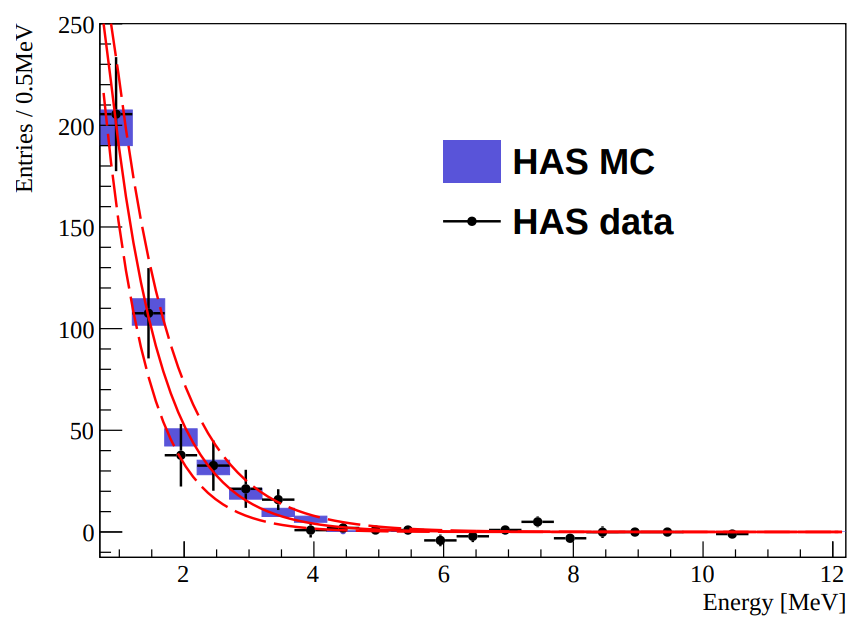
\includegraphics[scale=0.5]{Backgrounds/AmC/prompt_fit_data.png}
  \caption{Comparison of HAS prompt spectra from data and MC, showing the results of fitting the data to \autoref{eq:amc_fit_func}. From \cite{Gu_2016}.}
  \label{fig:amc_prompt_fit_data}
\end{figure}

\begin{figure}[ht]
  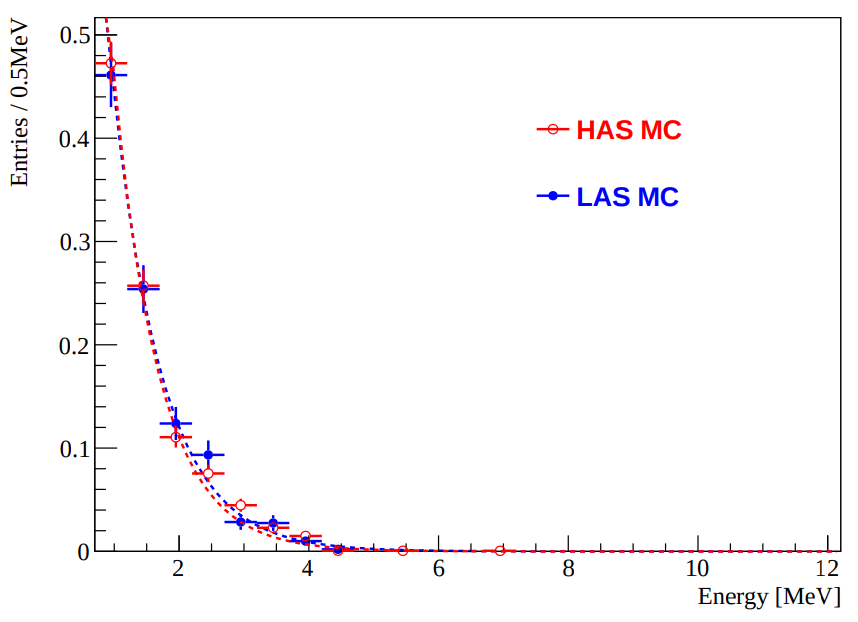
\includegraphics[scale=0.5]{Backgrounds/AmC/prompt_fit_mc.png}
  \caption{Comparison of HAS and LAS prompt spectra from the MC, showing the results of fitting the HAS spectrum to \autoref{eq:amc_fit_func}. From \cite{Gu_2016}.}
  \label{fig:amc_prompt_fit_mc}
\end{figure}

After the determination of $\xi$, the prompt spectrum (i.e. $p_1$), and the uncertainty, evaluation of each AD's AmC background then amounted to the simple task of measuring $R_{\mathrm{uncorr}}$ (after correcting for the muon veto efficiency) and multiplying it by $\xi$ according to \autoref{eq:bkgAmcFundamental}, resulting in the final values used in this analysis. It should be noted that the ACU-B and ACU-C AmC sources were removed from the EH3 ADs in 2012, during installation of EH2-AD2 and EH3-AD4.\footnote{In principle, the effective value of $\xi$ could vary between the three-sources and one-source scenarios, but this subtlety is not discussed in \cite{Gu_2016}. Presumably, any such effects fall within the 45\% uncertainty.} This significantly reduced the AmC background at the far site from 0.3\% to 0.1\% of the IBD rate. Furthermore, over the first two years of data, a 50\% decline was observed in the rate from each AmC source, in all three halls, likely due to leakage of scintillator into the source enclosures. This led to an ultimate background rate of only 0.03\% and 0.05\%\footnote{Within the single-digit precision of these percentages, the same value is obtained regardless of whether the denominator is chosen to be the signal rate or signal+background.}, near and far, respectively (although the mean rate over the entire data sample is higher, due to the fact that earlier rates were higher---0.05\% and 0.3\%, near and far, respectively.)

For the P17B data set used in this analysis, the AmC background rates were re-estimated by Wei in \cite{lianghongBkg} using updated measurements of the uncorrelated event rates from the AmC sources. The values are listed in \autoref{tab:bkgAmcDailyRates}.

\begin{table}[ht]
  \resizebox{\textwidth}{!}{%
   \begin{tabular}{lcccccccccc}
    \toprule
    & \multicolumn{2}{c}{EH1} & & \multicolumn{2}{c}{EH2} & & \multicolumn{4}{c}{EH3} \\
    \cmidrule{2-3} \cmidrule{5-6} \cmidrule{8-11}
    Period & AD1 & AD2 & & AD1 & AD2 & & AD1 & AD2 & AD3 & AD4 \\
    \midrule
    6AD & 0.29 $\pm$ 0.13 & 0.27 $\pm$ 0.12 & & 0.30 $\pm$ 0.14 & & & 0.24 $\pm$ 0.11 & 0.23 $\pm$ 0.10 & 0.23 $\pm$ 0.10 & \\
    8AD & 0.15 $\pm$ 0.07 & 0.15 $\pm$ 0.07 & & 0.12 $\pm$ 0.06 & 0.14 $\pm$ 0.06 & & 0.04 $\pm$ 0.02 & 0.03 $\pm$ 0.01 & 0.03 $\pm$ 0.02 & 0.04 $\pm$ 0.02 \\
    7AD & & 0.11 $\pm$ 0.05 & & 0.09 $\pm$ 0.04 & 0.08 $\pm$ 0.04 & & 0.02 $\pm$ 0.01 & 0.02 $\pm$ 0.01 & 0.03 $\pm$ 0.01 & 0.02 $\pm$ 0.01 \\ 
    \bottomrule
  \end{tabular}}
  \caption{AmC background rates for the P17B data set \cite{lianghongBkg}.}
  \label{tab:bkgAmcDailyRates}
\end{table}

\section{$\CanO$}
\label{sec:bkgCanO}

A final and relatively minor ($\lesssim$ 0.01\%/0.07\% near/far\footnote{As with the AmC background, the choice of denominator here (between signal and signal+background) makes no difference at the level of one significant figure.}) correlated background arises from $\alphN$ reactions initiated by natural radioactivity within the detector. In these reactions, an alpha particle from natural radioactivity is captured by a nucleus, which then emits a neutron. A prompt signal arises from a number of sources of energy deposition, including the kinetic energy of the alpha particle, gamma rays from nuclear deexcitation (including potentially those from inelastic scattering of the neutron), and proton recoils caused by the neutron. This prompt signal is then followed by capture of the neutron, mimicking the signature of an IBD. Our treatment of this background is based on that described in \cite{Zhao_2014} and \cite{An_2017}.

Based on the chemical composition of the scintillator and the known cross sections of $\alphN$ reactions, it was determined that $\CanO$ is the only such reaction to occur in the ADs at any significant rate. Meanwhile, there are three natural decay chains that can lead to alpha activity in the AD: The so-called uranium, thorium, and actinium chains, which begin, respectively, with the long-lived isotopes $^{238}$U, $^{232}$Th, and $^{235}$U\footnote{In practice, the rate of the thorium chain is determined by the concentration of the shorter-lived $^{228}$Th ($t_{1/2}$ = 1.9~yr), and likewise, for the actinium chain by $^{227}$Ac ($t_{1/2}$ = 21.8~yr).}. Given that U, Th, and Ac all have similar chemical properties to Gd, a small amount of contamination is difficult to avoid during the Gd-doping process. In addition to these three decay chains, additional alpha activity comes from the decay of $^{210}$Po, a moderately stable ($t_{1/2}$ = 138~d) daughter of $^{222}$Rn (which itself comes from the uranium chain). $^{210}$Po was deposited on detector surfaces by $^{222}$Rn during detector construction, and is essentially the only significant alpha emitter outside the GdLS region.

Quantifying the $\CanO$ background consists of two parallel tasks. One task is to determine the level of alpha activity produced by the three decay chains and by $^{210}$Po. The other task is to determine, for the set of alpha particles produced by a given chain (see \autoref{fig:aln_alpha_energy_dist}), the probability and prompt spectrum of the $\CanO$ events. These two pieces of knowledge can then be combined to yield a predicted rate and spectrum for the $\CanO$ background.

\begin{figure}[ht]
  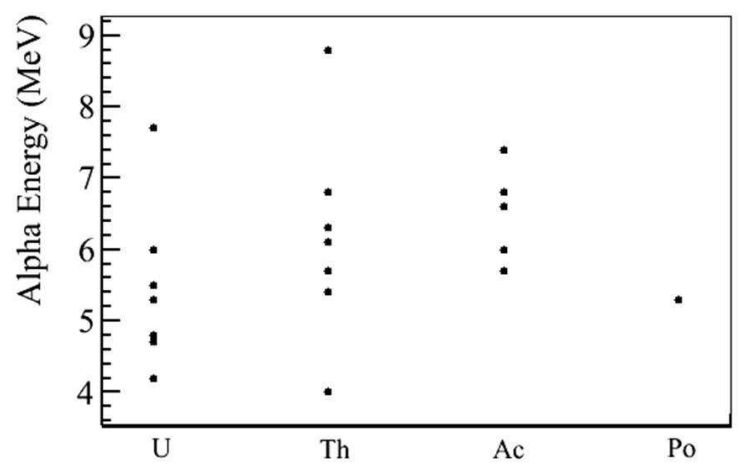
\includegraphics[scale=0.5]{Backgrounds/AlN/alpha_energy_dist.png}
  \caption{Distribution of $\alpha$ particle energies from decays of $^{238}$U, $^{232}$Th, $^{227}$Ac, and $^{210}$Po. From \cite{Zhao_2014}.}
  \label{fig:aln_alpha_energy_dist}
\end{figure}

The three chains all share a fortuitious property that enables a straightforward estimation of their rates. Namely, they each contain a rapid $\alpha$-$\alpha$ or $\beta$-$\alpha$ cascade whose time correlation and energy distribution allow for clean extraction from the data (\autoref{fig:aln_longpaper_bipo_sel}). For the uranium, thorium, and actinium chains, these cascades are, respectively, $^{214}$Bi $\to$ $^{214}$Po $\to$ $^{210}$Pb, $^{212}$Bi $\to$ $^{212}$Po $\to$ $^{208}$Pb, and $^{219}$Rn $\to$ $^{215}$Po $\to$ $^{211}$Pb, with Po half-lives of \SI{164.3}{\micro s}, \SI{0.3}{\micro s}, and \SI{1.781}{ms}, respectively.

\begin{figure}[ht]
  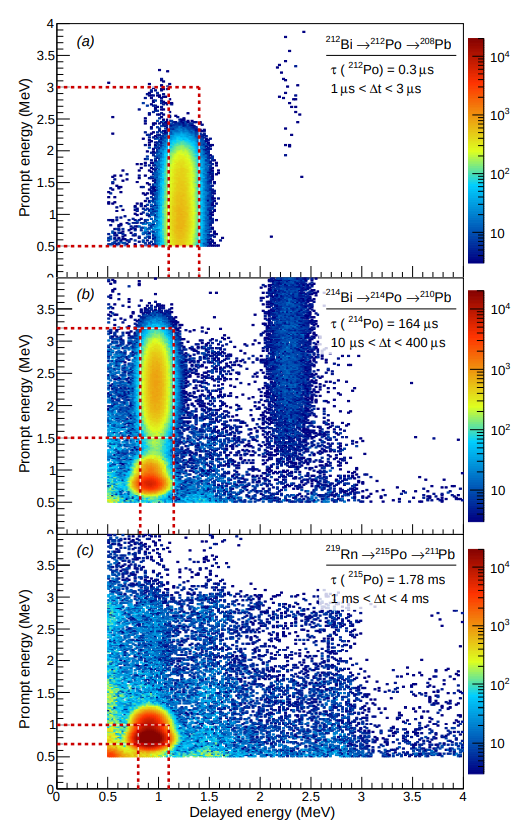
\includegraphics[scale=0.5]{Backgrounds/AlN/longpaper_bipo_sel.png}
  \caption{Illustration of the prompt and delayed energy distributions for the Bi-Po cascades used in determining the rates of the $^{238}$U, $^{228}$Th, and $^{227}$Ac decay chains. From \cite{An_2017}.}
  \label{fig:aln_longpaper_bipo_sel}
\end{figure}

To extract these events, time coincidence windows of [10, 400]~\us, [1, 3]~\us, and [1, 4]~ms were used, respectively \cite{An_2017}.\footnote{It is curious that, for the case of $^{212}$Po (i.e. $^{232}$Th), the time window used is significantly larger, relative to the half-life, compared to the other two isotopes. As shown in \autoref{fig:aln_longpaper_bipo_sel}, the $^{212}$Po sample is the ``cleanest'' (in terms of accidental backgrounds), enabling the use of a (perhaps excessively) wide window in order to maximize the statistics. Since Th is the most active chain, maximal statistics are desirable.} Accidentals (most significant for the actinium chain's Po cascade) were subtracted via the usual procedure,
% (YYY check that this was actually done, at least for actinium),
and for the uranium chain's Po cascade, contamination with nH IBDs was not an issue given that the (quenched) delayed energy of the alpha particle for these events is around 1-1.5~MeV, significantly below the 2.2-MeV gamma ray from nH capture. For the thorium chain, the prompt spectrum had to be extrapolated below 0.5~MeV in order to determine the total rate; otherwise, there were no major complications. Under the assumption that each chain is in equilibrium\footnote{Up to $^{228}$Th and $^{227}$Ac for the thorium and actinium chains, rather than all the way up to $^{232}$Th and $^{235}$U, as noted previously.}, the rate of the polonium cascade gives the rate of the entire chain.

At the point in time when Daya Bay began taking data, this procedure determined average (across ADs) rates of 0.009, 0.2, and 0.02~Bq for U, Th, and Ac, respectively \cite{lianghongBkg}. Since the U chain is initiated by $^{238}$U in the AD, its rate is essentially constant, given the $^{238}$U half-life of 4.5~Gyr. On the other hand, the Th and Ac rates do decrease over time, since the parent half-lives (i.e. those of $^{228}$Th and $^{227}$Ac) are 1.9 and 21.8~yr, respectiely. To determine the average Th and Ac rates for the P17B dataset used in this analysis, Wei in \cite{lianghongBkg} repeated the Bi-Po cascade selection and obtained AD-averaged rates of 0.136 and 0.0178~Bq for $^{228}$Th and $^{227}$Ac, respectively.
% \footnote{Given the difference in half-lives between the two isotopes, one would expect a greater difference in the rate decrease than that measured by Wei. However, this discrepancy is encompassed by the uncertainty of the rate measurement procedure.}

For $^{210}$Po, a single decay instead of a chain, time correlations could not be exploited. Instead, the 5.3~MeV alpha particle produced by this isotope was, after quenching, visible as a peak around 0.5~MeV in the singles spectrum. Fitting this peak gave rates ranging from 4--10~Hz for each AD \cite{zeyuanAln}. Although the $^{210}$Po half-life is only 138 days, its parent, $^{210}$Pb (which determines the $^{210}$Po rate decrease over time), has a 22.3-year half-life. Within the precision of the measurement procedure, the decrease of the $^{210}$Po rate was unobservable.

For a given decay chain (or $^{210}$Po decay), the set of emitted alpha particles is known (\autoref{fig:aln_alpha_energy_dist}). For each of these alpha particles, in turn, simulations (using Geant4 \cite{Geant4} and SRIM \cite{SRIM}) can be used to determine the rate and prompt spectrum of the $\CanO$ events. At each step in the simulation, the alpha particle loses some energy and travels some distance according to its $dE/dx$ profile in the LS. With some probability (i.e. cross section), during this step the alpha particle may be captured, producing one of the excited states of $^{17}$O. If this happens, the $^{17}$O will emit a neutron, whose energy depends on both the initial excited state of $^{17}$O and the final (excited or ground) state of $^{16}$O. The neutron produces prompt energy through proton recoils and, if it is sufficiently energetic, may scatter inelastically on $^{12}$C to produce a $\sim$5~MeV gamma ray. Additional prompt energy will come from deexcitation gamma rays if the $^{16}$O had been produced in an excited state.

The simulation calculates the (very low) probability of an $(\alpha,\mathrm{n})$ reaction occurring for a single cascade of alpha particles in a given chain (\autoref{tab:bkgAlnNeutronYield}). The simulation also produces, for the $(\alpha,\mathrm{n})$ reactions from a given chain, the 2D PDF of (a) the amount of energy deposited in the scintillator and (b) the kinetic energy of the emitted neutron (illustrated in \autoref{fig:aln_energy_pdf}). Finally, the prompt energy spectrum (\autoref{fig:aln_longpaper_prompt_spec}) is obtained by sampling this PDF and performing MC simulations of the detector's response to the alpha particle, the neutron's recoil protons, and any gamma rays from $^{12}$C inelastic scattering and $^{16}$O$^*$ deexcitation.

\begin{table}[ht]
  \begin{tabular}{lcccc}
    \toprule
    Chain & $N_{\mathrm{ground}}$ & $N_{\mathrm{excited}}$ & $N_{\mathrm{total}}$ & Uncertainty  \\
    \midrule
    $^{210}$Po & 5.26e-8 & 4.90e-9 & 5.75e-8 & 7.2\%  \\
    $^{238}$U  & 4.34e-7 & 2.96e-7 & 7.30e-7 & 16.9\% \\
    $^{228}$Th & 4.49e-7 & 4.92e-7 & 9.41e-7 & 27.7\% \\
    $^{227}$Ac & 4.72e-7 & 6.18e-7 & 1.09e-6 & 25.9\% \\
    \bottomrule
  \end{tabular}
  \caption{Neutron yield (i.e., number of $(\alpha,\mathrm{n})$ events) per decay chain. $N_{\mathrm{ground}}$ and $N_{\mathrm{excited}}$ refer to the number of events that leave $^{16}$O in the ground and excited states, respectively. $N_{\mathrm{total}}$ is their sum, whose uncertainty is given in the final column. From \cite{Zhao_2014}.}
  \label{tab:bkgAlnNeutronYield}
\end{table}

\begin{figure}[ht]
  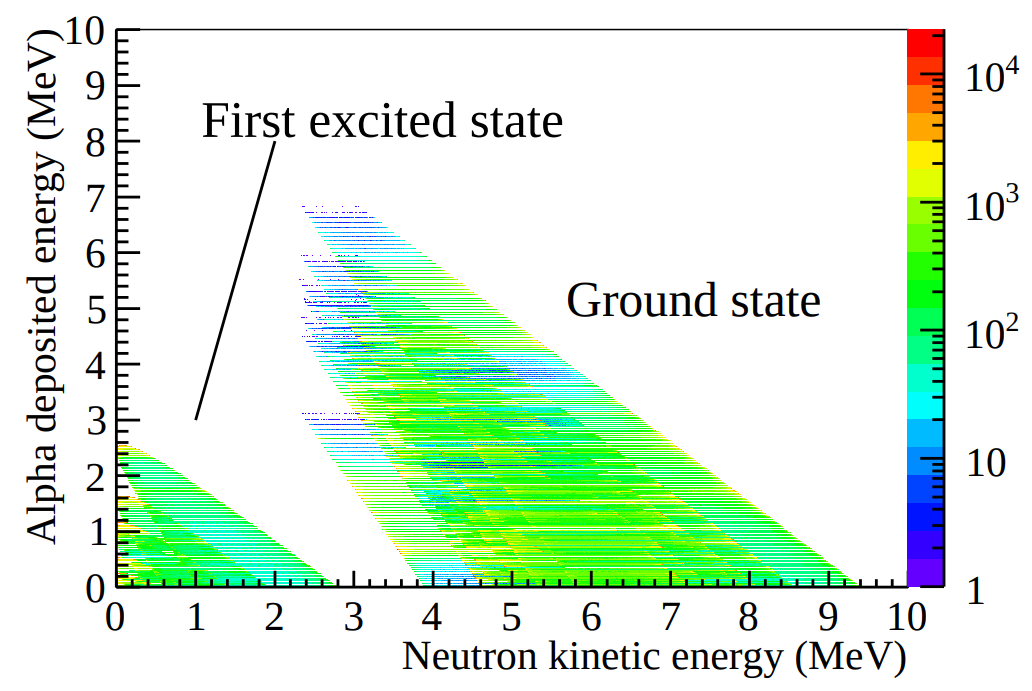
\includegraphics[scale=0.45]{Backgrounds/AlN/energy_pdf.png}
  \caption{2D probability distribution function of alpha particle energy deposition and neutron kinetic energy for $(\alpha,\mathrm{n})$ reactions from the $^{228}$Th chain. From \cite{Zhao_2014}.}
  \label{fig:aln_energy_pdf}
\end{figure}

\begin{figure}[ht]
  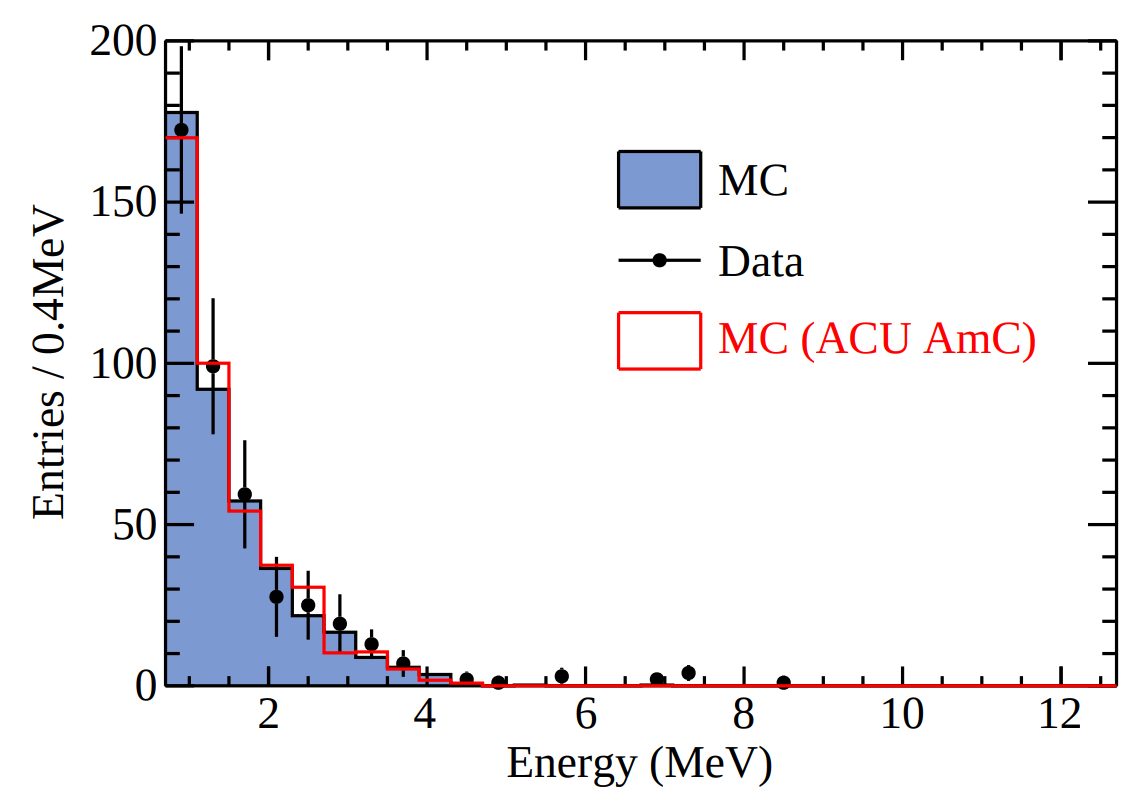
\includegraphics[scale=0.5]{Backgrounds/AlN/longpaper_prompt_spec}
  \caption{Prompt energy spectra, as determined by simulation, for $(\alpha,\mathrm{n})$ reactions produced by the four decay chains. From \cite{An_2017}.}
  \label{fig:aln_longpaper_prompt_spec}
\end{figure}

Uncertainties in the $\CanO$ prediction arise from a number of sources. The uncertainty coming from the $\alphN$ cross section was estimated by repeating the MC procedure using two different cross section tables, JENDL \cite{jendl} and EXFOR \cite{exfor} (\autoref{fig:aln_xsec}). This suggested an uncertainty ranging from 6.6\% (for $^{210}$Po) up to 27.5\% (for $^{232}$Ac) \cite{Zhao_2014}; a nominal uncertainty of 20\% was thus assigned. Meanwhile, there was negligible effect on the predicted neutron reconstructed energy spectrum from switching between the cross section tables and the assumed neutron angular distribution (\autoref{fig:aln_n_vis_spectra}). Additional uncertainty could come from the fundamentals of the MC simulation, i.e., the $dE/dx$ table and the numerical integration of discrete steps. This was evaluated by comparing the results of Geant4 \cite{Geant4} and SRIM \cite{SRIM} (\autoref{fig:aln_n_kin_spectra}), which differed, overall, at a negligible level of less than a percent. Finally, the assumption of decay chain equilibrium, and the efficiency of the cascade selection, both could introduce additional uncertainty, leading to the conservative assignment of an overall 30\% uncertainty\footnote{Presumably validated by varying the Bi-Po cascade selection criteria, although this is not explicitly stated in the references.} in the measurement of the rates of the decay chains. This 30\% uncertainty is combined with the 20\% uncertainty assigned to the neutron yield calculation; conservatively adding the two uncertainties then gives a total uncertainty of 50\% on the $\CanO$ rate estimation.

\begin{figure}[ht]
  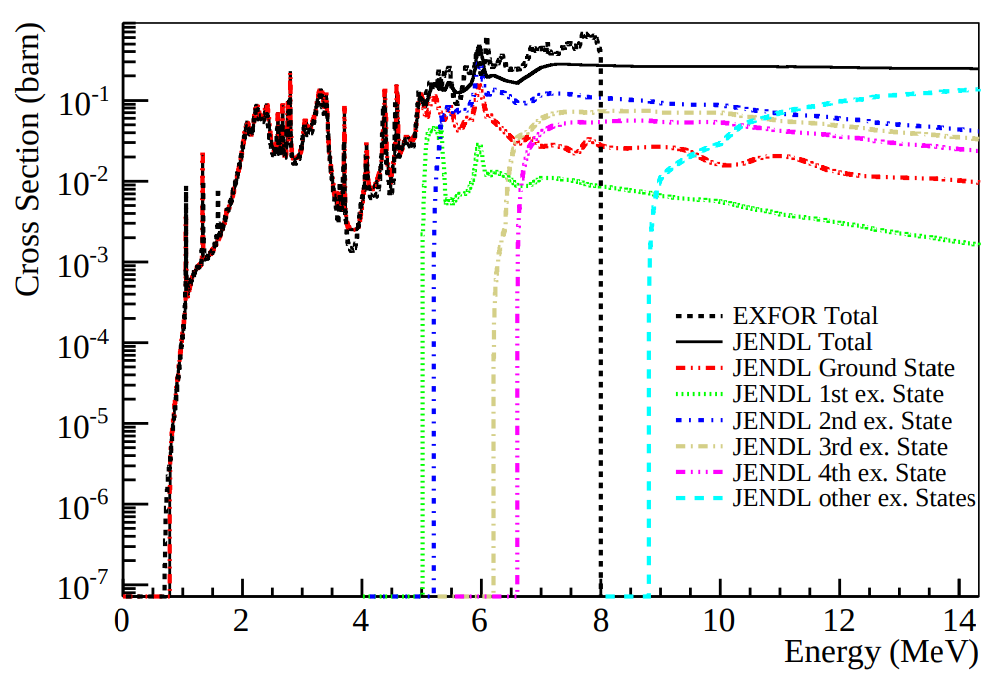
\includegraphics[scale=0.5]{Backgrounds/AlN/xsec.png}
  \caption{Cross section of the $\CanO$ reaction as reported by the JENDL and EXFOR tables. From \cite{Zhao_2014}.}
  \label{fig:aln_xsec}
\end{figure}

\begin{figure}[ht]
  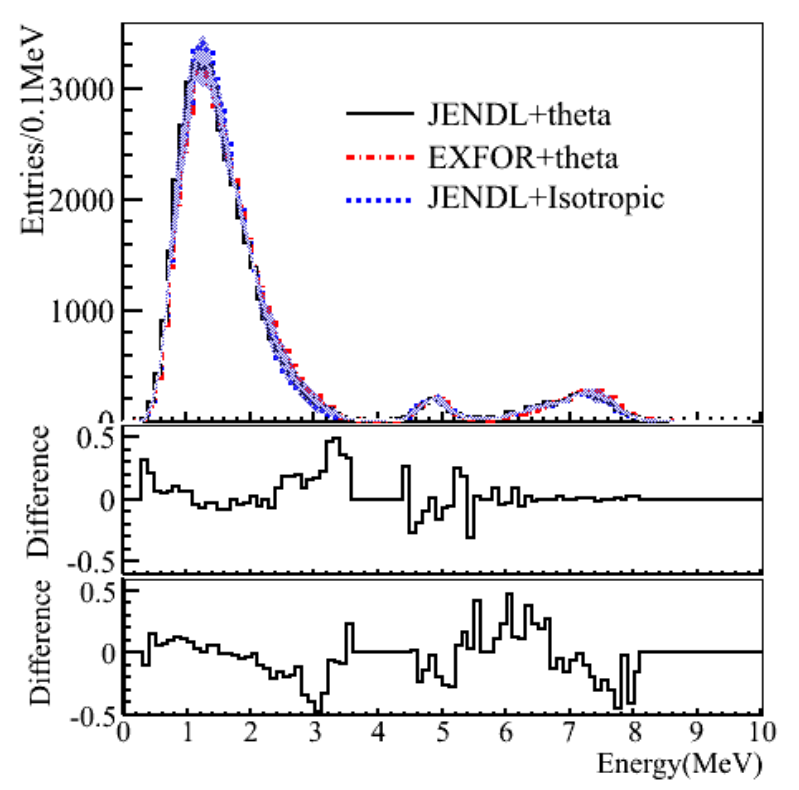
\includegraphics[scale=0.5]{Backgrounds/AlN/n_vis_spectra.png}
  \caption{Predicted neutron reconstructed energy for different cross section tables (JENDL and EXFOR) and different neutron angular distributions (``theta'', $d\sigma/d\Omega \sim 1/\sin\theta$, and ``isotropic'', $d\sigma/d\Omega \sim 1$). The differences are negligible. From \cite{Zhao_2014}. (The particular decay chain is not specified.)}
  \label{fig:aln_n_vis_spectra}
\end{figure}

\begin{figure}[ht]
  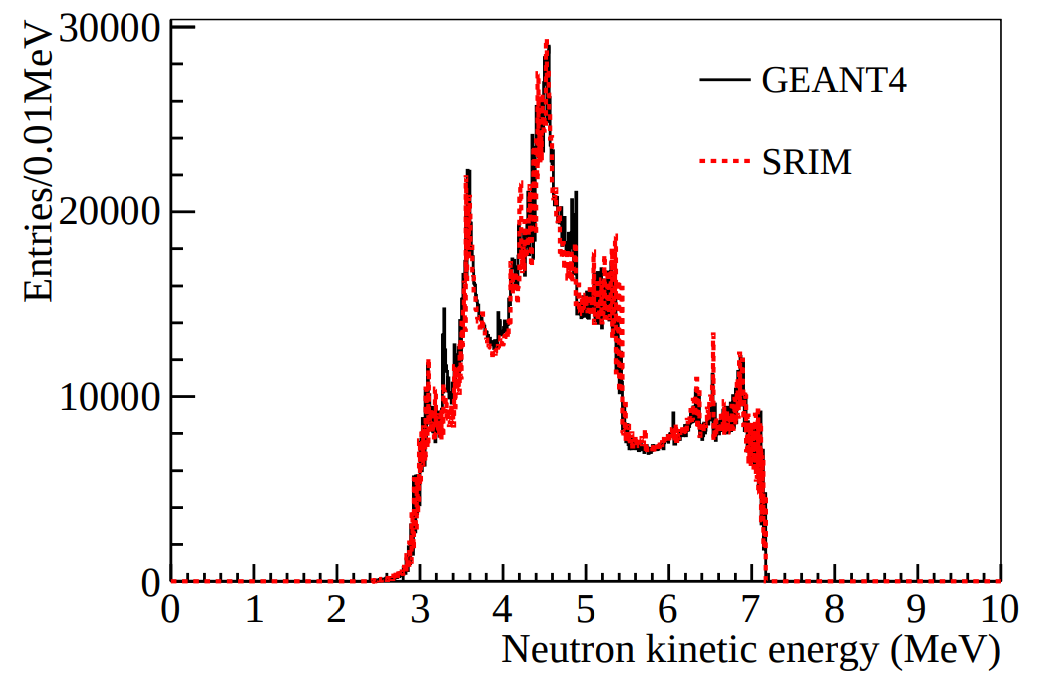
\includegraphics[scale=0.45]{Backgrounds/AlN/n_kin_spectra.png}
  \caption{Neutron kinetic energy as predicted by Geant4 and SRIM. From \cite{Zhao_2014}. (The particular decay chain is not specified.)}
  \label{fig:aln_n_kin_spectra}
\end{figure}

For the P17B data set used in this analysis, the $\CanO$ background rates were re-estimated by Wei in \cite{lianghongBkg} using updated measurements of the rates of alpha activity. The values are listed in \autoref{tab:bkgAlnDailyRates}.

\begin{table}[ht]
  \resizebox{\textwidth}{!}{%
    \begin{tabular}{lcccccccccc}
      \toprule
      & \multicolumn{2}{c}{EH1} & & \multicolumn{2}{c}{EH2} & & \multicolumn{4}{c}{EH3} \\
      \cmidrule{2-3} \cmidrule{5-6} \cmidrule{8-11}
      Period & AD1 & AD2 & & AD1 & AD2 & & AD1 & AD2 & AD3 & AD4 \\
      \midrule
      6AD & 0.09 $\pm$ 0.04 & 0.07 $\pm$ 0.04 & & 0.05 $\pm$ 0.02 & & & 0.05 $\pm$ 0.02 & 0.04 $\pm$ 0.02 & 0.04 $\pm$ 0.02 & \\
      8AD & 0.08 $\pm$ 0.04 & 0.06 $\pm$ 0.03 & & 0.04 $\pm$ 0.02 & 0.06 $\pm$ 0.03 & & 0.04 $\pm$ 0.02 & 0.04 $\pm$ 0.02 & 0.03 $\pm$ 0.02 &  0.04 $\pm$ 0.02 \\
      7AD & & 0.05 $\pm$ 0.03 & & 0.03 $\pm$ 0.02 & 0.06 $\pm$ 0.03 & & 0.03 $\pm$ 0.02 & 0.03 $\pm$ 0.02 & 0.03 $\pm$ 0.01 & 0.03 $\pm$ 0.02 \\
      \bottomrule
    \end{tabular}}
  \caption{$\CanO$ background rates for the P17B data set \cite{lianghongBkg}.}
  \label{tab:bkgAlnDailyRates}
\end{table}

% \section{Summary of backgrounds}
% \label{sec:bkgSummary}

\end{document}
